\documentclass[a4paper,11pt]{article}
\pdfoutput=1 % if your are submitting a pdflatex (i.e. if you have
             % images in pdf, png or jpg format)

\usepackage{jcappub}
\usepackage{graphicx}
\usepackage{dcolumn}
\usepackage{amssymb,amsmath,bm}
\usepackage{color}
\usepackage[dvipsnames]{xcolor}
%\usepackage[colorlinks,linkcolor=red,citecolor=blue,urlcolor=blue ]{hyperref}
%\usepackage[utf8]{inputenc}
\usepackage{lipsum}
\usepackage{xfrac}
\usepackage{aas_macros}
\usepackage{mathrsfs}
\usepackage{subfigure}
\usepackage{rotating}
\newcommand{\nv}{\vec{\theta}}
%\newcommand{\pasj}{Publications of the ASJ}
%\newcommand{\aap}{Astronomy and Astrophysics}
%\newcommand{\apj}{Astrophysical Journal}
%\newcommand{\apjs}{Astrophysical Journal, Supplement}
%\newcommand{\mnras}{Monthly Notices of the RAS}
\newcommand{\todo}[1]{{\bf TODO: #1}}

\newcommand{\as}[1]{{\textcolor{blue}{[AS: #1]}}}
\newcommand{\an}[1]{{\textcolor{magenta}{[AN: #1]}}}
\newcommand{\da}[1]{{\textcolor{red}{[DA: #1]}}}

\newcommand\Tstrut{\rule{0pt}{3ex}}   

\definecolor{internationalkleinblue}{rgb}{0.0, 0.18, 0.65}
\hypersetup{urlcolor=internationalkleinblue, linkcolor=internationalkleinblue, citecolor=internationalkleinblue}

\usepackage[T1]{fontenc} % if needed
\usepackage{natbib}
\bibliographystyle{JHEP}
\title{Tomographic galaxy clustering with the Subaru Hyper Suprime-Cam first year public data release}

\author[a,1]{Andrina Nicola,}
\author[b]{David Alonso,}
\author[c]{An\v{z}e Slosar,}
\author[d]{Humna Awan,}
\author[d]{Adam Broussard,}
\author[b]{Zahra Gomes,}
\author[d]{Eric Gawiser,}
\author[x]{Rachel Mandelbaum,}
\author[x]{Hironao Miyatake,}
\author[e]{Jeffrey A. Newman,}
\author[f,g]{Javier S\'anchez,}
\author[x]{Ignacio Sevilla,}
\author[c,h]{Sarah Skinner,}
\author[x]{Erica Wagoner}

\affiliation[a]{Department of Astrophysical Sciences, Princeton University, Peyton Hall, Princeton NJ 08544-0010, USA}
\affiliation[b]{Department of Physics, University of Oxford, Denys Wilkinson Building, Keble Road, Oxford OX1 3RH, United Kingdom}
\affiliation[c]{Brookhaven National Laboratory, Physics Department, Upton, NY 11973, USA}
\affiliation[d]{Rutgers University, Physics \& Astronomy Department, Piscataway, NJ 08854, USA}
\affiliation[e]{Department of Physics and Astronomy and PITT PACC, University of Pittsburgh, Pittsburgh, PA, 15260, USA}
\affiliation[f]{Fermi National Accelerator Laboratory, Batavia, IL, 60510, USA}
\affiliation[g]{Department of Physics and Astronomy, University of California, Irvine, CA 92697, USA}
\affiliation[h]{Department of Physics, Missouri University of Science and Technology, Rolla, MO 65401, USA}

\emailAdd{anicola@astro.princeton.edu}

\abstract{We analyze the clustering of galaxies in the first public data release of the Hyper Suprime-Cam Subaru Strategic Program. Despite the relatively small footprints of the observed fields, the data are an excellent proxy for the very deep photometric datasets as will be acquired by the Large Synoptic Survey Telescope, and are therefore an ideal test bed for the analysis methods being implemented by the Dark Energy Science Collaboration. We select a magnitude limited sample with $i<24.5$ and analyze it in four tomographic redshift bins covering the range $0.15\lesssim z\lesssim1.5$. We carry out a Fourier-space analysis of the two-point clustering of this sample, including all auto- and cross-correlations between bins. We demonstrate the use of map-level deprojection methods to account for non-physical fluctuations in the galaxy number density caused by observational systematics. Through a halo occupation distribution analysis, we place constraints on the characteristic halo masses of this sample as a function of redshift, finding a good fit up to scales $k_{\rm max}=1\,{\rm Mpc}^{-1}$, including both auto- and cross-correlations. Our results show monotonically decreasing average halo masses, which can be interpreted in terms of the drop-out of red galaxies at high redshifts for a flux-limited sample, reproducing previous results. In terms of photometric redshift systematics, we show that additional care is needed in order to marginalize over uncertainties in the redshift distribution in galaxy clustering, even for samples of this small size, and that these uncertainties can be significantly constrained by including cross-bin correlations. We are able to make a $\sim3\sigma$ detection of the effects of lensing magnification in the HSC data. When freeing up cosmological parameters, we find constraints on the amplitude of density fluctuations $\sigma_8$ and the cold dark matter abundance $\Omega_c$ that agree well with measurements from Planck and low-redshift probes. Finally, we use our analysis pipeline to study the clustering of galaxies as a function of limiting flux, and provide a simple model for the linear galaxy bias for magnitude limited samples as a function of limiting magnitude and redshift.}

\begin{document}
\maketitle
\flushbottom

\section{Introduction}\label{sec:intro}

The past two decades have seen a revolution in our understanding of the universe and its constituents. While observations of the cosmic microwave background play a pivotal role \cite{Planck:2018}, they are only indirectly sensitive to physics of the low redshift universe, in particular to the expansion history and growth, which are uniquely sensitive to properties of dark energy and modified gravity \cite{1903.12016}.

In studies of the low redshift universe, surveys of the large scale structure play an increasingly important role. Over a decade ago, the Dark Energy Task Force has divided the evolution of optical experiments into approximate stages \cite{0609591}. The current Stage III experiments, including spectroscopic surveys such as eBOSS \cite{1707.09322,1801.03038,1712.08064,1801.02689,1801.02891} and VIPERS \cite{1611.07048,1612.05645,1708.00026} and photometric surveys such as DES \cite{1708.01531,1708.01530,1708.01536}, Hyper Suprime-Cam \cite{1704.05858,2019PASJ...71...43H,1906.06041} and the Kilo-Degree Survey / VIKING-450 \cite{1902.11265,1812.06077,Joudaki:2019} are approaching completion and the field is preparing for the Stage IV surveys, such as DESI \cite{1611.00036,1907.10688} and LSST \cite{0912.0201,1809.01669} as well as major satellite missions like Euclid \cite{1606.00180} and WFIRST \cite{1904.01174}.

Together with transformational sensitivity increases in the Stage IV surveys, the challenges of understanding and controlling systematic errors are becoming considerably more difficult \cite{1808.07335}. For photometric surveys, the deep surveys sensitive to many more sources inevitably come with crowded fields where effects of blending affect a significant fraction of all sources in the field. The increased blending leads to new uncertainties in isolating sources, measuring their fluxes (required for photometric redshifts) and inferring their shear estimates. These effects in turn lead to subtle sample selection effects, which are amplified by the interaction of the point spread function with blending \cite{1708.01533,1905.01324,1907.10572}. But even with perfect measurements of fluxes, our ability to infer redshift distribution of sources is hampered by incompleteness in spectroscopic samples used to calibrate redshifts \cite{1903.09325}. Finally, at the depths of Stage IV photometric surveys, instrumental and observational effects, such as the scattered light from bright objects, errors in the galaxy-star separation, reddening by the milky way dust and others will impriment their own fluctuations into the galaxy density of objects. These fluctuations will, if not correctly accounted for, masquerade as intrinsic large-scale fluctuations in the cosmic density fields.  Therefore, Stage IV photometric experiments are likely to be limited by our ability to control systematics rather than the intrinsic statistical power of the survey.

Community is well aware of these challenges lying ahead. There are two main approaches that are being used in preparation for the arrival of data. On one hand, we are building very sophisticated realistic mock data sets, such as LSST DESC Data Challenge 2 \cite{1909.07340,1907.06530}. On the other hand, we are re-analyzing the existing precursor data to test-drive our methods and codes in realistic environment. In this paper we focus on the latter approach using Hyper Suprime-Cam Subaru Strategic Program (HSC-SSP) first data release  \cite{2018PASJ...70S...8A}. The main advantage of this dataset is that it is in many respects very similar to the LSST data, both in terms of depth and bands as well as primary data reduction and catalog generation. It covers essentially the same bands as LSST, with the exception of missing the UV $u$-band fluxes, which are unlikely to play a major role in cosmological data analysis. We will work with limiting magnitude for 5-$\sigma$ source detection of $i<24.5$, similar to expected magnitude cut to be used for LSST of $i<25.1$ after 1 year \cite{1809.01669}.  The primary data reduction codes used in HSC-SSP and planned for LSST are of the same lineage employing much of the same methods \cite{2018PASJ...70S...5B,1812.03248}. With the exception of a rather small sky area of around 90 square degrees used in this paper, the HSC-SSP data is a perfect example of how the LSST data will look like.


In this paper we focus exclusively on the galaxy clustering part of the data analysis. While the statistically most powerful data combination includes the full 3$\times$2 point analysis (i.e. shear and number density auto and cross-correlations), galaxy clustering along comes with unique challenges, which are the focus of this paper. In particular, galaxy clustering is more sensitive to details of redshift distribution of sources and systematic effects that can generate false fluctuations in number densities. These are the main effects that we study in this paper. We will employ basic tools of the trade, such as measuring power spectrum using mode deprojection and then fit the resulting data taking into account possible deviations from redshift distribution estimates. The question is whether there are sufficient given the statistical precision of the data. We will find that the answer is yes, at least over the total area of HSC-SSP DR1 data.

Due to rather small area, we will be employing simple semi-analytical halo model to make theory predictions. While this model is most certainly not sophisticated enough for the full sky LSST analysis, it suffices for the statistical precision of data at hand. While we will derive some useful constraints on the halo model parameters, the use of halo model here should be viewed as a ``good enough'' substitute for the final modeling, which will likely include bias expansion approaches \cite{0902.0991,1402.5916,1611.09787} and power spectrum emulators \cite{1804.05865,1705.03388}.


The paper is structured as follows.  In Section \ref{sec:data}, we discuss the HSC-SSP data and how we process it in order to generate a set of galaxy over-density maps together with maps of potential systematics. In Section \ref{sec:methods}, we detail the methodology employed in our analysis and in Section \ref{sec:results}, we present results alongside numerous tests. We discuss and conclude in Section \ref{sec:discussion}.

\section{Data}\label{sec:data}
  \begin{table}
  \centering
  \begin{tabular}{|l|l|}
  \hline
   {\bf Cut} & {\bf Comment} \\
   \hline
   \texttt{detect\_is\_primary}=True & Basic quality cuts, \\
   \texttt{icmodel\_flags\_badcentroid}=False & see \cite{2018PASJ...70S..25M,2018PASJ...70S...5B}\\
   \texttt{icentroid\_sdss\_flags}=False & \\
   \texttt{iflags\_pixel\_edge}=False & \\
   \texttt{iflags\_pixel\_interpolated\_center}=False & \\
   \texttt{iflags\_pixel\_saturated\_center}=False & \\
   \texttt{iflags\_pixel\_cr\_center}=False & \\
   \texttt{iflags\_pixel\_bad}=False & \\
   \texttt{iflags\_pixel\_suspect\_center}=False & \\
   \texttt{iflags\_pixel\_clipped\_any}=False & \\
   \texttt{meas.ideblend\_skipped}=False & \\
   \texttt{iblendedness\_abs\_flux}$<10^{-0.375}$ & \\
   \hline % Strict from here on
   \texttt{[g,r,z,y]centroid\_sdss\_flags}=False & Strict photometry cuts\\
   \texttt{[g,r,i,z,y]cmodel\_flux\_flags}=False & \\
   \texttt{[g,r,i,z,y]flux\_psf\_flags}=False & \\
   \texttt{[g,r,z,y]flags\_pixel\_edge}=False & \\
   \texttt{[g,r,z,y]flags\_pixel\_interpolated\_center}=False & \\
   \texttt{[g,r,z,y]flags\_pixel\_saturated\_center}=False & \\
   \texttt{[g,r,z,y]flags\_pixel\_cr\_center}=False & \\
   \texttt{[g,r,z,y]flags\_pixel\_bad}=False & \\
   \hline
   \texttt{icmodel\_mag}$-$\texttt{a\_i} $<$ 24.5 & Magnitude limit\\ % Magnitude cut
   \hline
   \texttt{icmodel\_flux}$>10\,$\texttt{icmodel\_flux\_err} & 10$\sigma$ detections\\
   \hline
   \texttt{[g,r,y,z]cmodel\_flux}$>5\,$\texttt{[g,r,y,z]cmodel\_flux\_err} & 5$\sigma$ detection  (required \\
   & only in 2 other bands)\\
   \hline
   \texttt{iclassification\_extendedness}=1 & Star-galaxy separator\\
   \hline
  \end{tabular}
  \caption{Summary of the selection cuts performed to the original dataset to retrieve the sample considered in our analysis.} \label{tab:cuts_summary}
  \end{table}  

  \begin{table}
  \centering
  \begin{tabular}{|l|r|c|l|}
   \hline
   {\bf Field name} & $N_{\rm gal}$ & {\bf Area} (deg$^2$) & $f_{\rm sky}$ \\
   \hline
   GAMA09H  & 1,697,713 & 14.5 & $3.5\times10^{-4}$ \\
   GAMA15H  & 1,695,364 & 15.1 & $3.7\times10^{-4}$ \\
   HECTOMAP &   639,970 &  5.1 & $1.2\times10^{-4}$ \\
   VVDS     & 2,340,965 & 20.6 & $5.0\times10^{-4}$ \\
   WIDE12H  & 1,220,816 & 11.6 & $2.8\times10^{-4}$ \\
   XMMLSS   & 2,139,629 & 20.8 & $5.0\times10^{-4}$ \\
   \hline
   Total    & 9734457 & 87.7 & $2.1\times10^{-3}$ \\
   \hline
  \end{tabular}
  \caption{Summary of the 6 different fields used in our analysis. The second column lists the number of galaxies in the DR1 catalog passing the cuts in Table \ref{tab:cuts_summary}. The third and fourth columns show the area and corresponding sky fraction covered by each field. The area was calculated as the sum of pixel areas allowed by the sky mask described in Section \ref{ssec:methods.mask}. \an{We don't use HECTOMAP in the fitting. Shall we even show it here?}} \label{tab:field_summary}
  \end{table}  

  \begin{table}
  \centering
  \begin{tabular}{|l|l|l|l|}
    \hline
    $z_{\rm phot}^{\rm ini}$ & $z_{\rm phot}^{\rm end}$ & $\bar{z}$ & $N_{\rm gal}$ \\
    \hline
    0.15 & 0.5  & 0.57 & 1,750,274 \\
    0.5  & 0.75 & 0.68 & 1,766,939 \\
    0.75 & 1.0  & 0.91 & 1,702,685 \\
    1.0  & 1.5  & 1.26 & 1,752,359 \\
    \hline
  \end{tabular}
  \caption{Summary of the 4 redshift bins used in our analysis. The first two columns show the photo-$z$ bin edges. We used the {\tt photoz\_best} redshift estimator for the photo-$z$ code {\tt ephor\_ab} to assign galaxies to different bins. The second column shows the mean redshift of each bin calculated from the fiducial redshift distributions described in Section \ref{ssec:methods.nz}. The last column shows the number of galaxies in each bin. The bin edges were chosen to roughly contain an equal number of galaxies in each of them.} \label{tab:bins_summary}
  \end{table}
  
  We use data from the Hyper Suprime-Cam Subaru Strategic Program first data release (HSC DR1 hereon)\footnote{https://hsc-release.mtk.nao.ac.jp}. The release is extensively documented in \cite{2018PASJ...70S...8A}, and we only provide the details of the galaxy sample and associated data used for our clustering analysis.

  HSC-SSP is a photometric galaxy survey that has been awarded 300 nights on the Subaru Telescope starting in 2014. DR1 includes data from 61.5 nights covering and comes with fields of three depths: Wide (108 square degrees to $i\sim 26.4$), Deep (26 square degrees to $i\sim26.5$) and UltraDeep (4 square degrees to $i\sim 27$). In this work we focus on the Wide field, which has been observed in five broadband filters ($grizy$) and is distributed among 7 fields between 5 and 20 square degrees each. The image quality is impressive at median seeing of around 0.6 arcsec, which is considerably better than other comparable surveys (e.g. DES with around 0.9 arc sec) and also likely better than median seeing that will be achieved by LSST. The data are processed with \texttt{hscPipe} \cite{2018PASJ...70S...5B} and  available to the community as a publicly available database.

  
  We use a magnitude-limited sample constructed from the WIDE DR1 sample by imposing data cuts that are similar to those used to create the HSC shear catalog \cite{2018PASJ...70S..25M}. The exact cuts are shown in Table~\ref{tab:cuts_summary}, and can be summarized as follows: besides a minimal set of quality cuts (selecting only primary detections with well-measured fluxes in all bands, removing objects near bad pixels, deblender artifacts, etc.), we impose an overall apparent magnitude cut in the extinction-corrected band $i_{\rm corr}<24.5$. This choice was based on a study of the survey depth-completeness relation in order to select a homogeneous and complete sample of high-confidence ($>10\sigma$) detections (see Section \ref{ssec:methods.syst}). We also select only objects with significant detections ($>5\sigma$) in at least two of the 4 remaining bands ($g,\,r,\,z,\,y$), and remove all objects classified as stars by the data reduction pipeline, using the "extendedness`` classifier as described in \cite{2018PASJ...70S..25M,2018PASJ...70S...5B}. The resulting sample consists of 9,734,457 objects and covers $\sim88$ square degrees distributed across the 6 HSC DR1 fields, as described in Table \ref{tab:field_summary}.

  All objects have photometric redshift measurements from 6 different codes as presented in \cite{2018PASJ...70S...9T}. We use the {\tt photoz\_best} redshift estimator assigned by the {\tt ephor\_ab} method as a marker to divide the sample into four tomographic samples containing roughly equal numbers of galaxies. The {\tt photoz\_best} estimator is defined to minimize the risk that the true galaxy redshift lies outside the range $z_{\rm true}\pm 0.15(1+z_{\rm true})$, where $z_{\rm true}$ is the galaxy's true redshift. A preliminary Fisher matrix study showed that the information content saturates quickly when slicing the data into more than four samples. The redshift bins are described in Table \ref{tab:bins_summary}, and the associated redshift distributions are discussed in Section \ref{ssec:methods.nz}.

\section{Methods}\label{sec:methods}

Our basic method is to measure the two point function of all possible combinations of galaxy density fluctuation fields. We work in the Fourier domain, so our basic quantity is the angular power spectrum $C_\ell$. Given four tomographic samples, our measurement consists of four auto power spectra and six cross-power spectra. In this section we discuss how we construct maps of galaxy density fluctuations and associate maps of potential systematics , how we use these to measure the power spectra and its covariance matrix and finally how these are modeled within the context of halo model.


  \subsection{Pixels and maps}\label{ssec:methods.pix}
    Our $C_\ell$-based analysis requires us to make maps of different quantities. The HSC DR1 is distributed across the 6 small fields ($\lesssim20\,{\rm deg.}^2$) summarized in Table \ref{tab:field_summary}. In this case, storing maps covering the full sky down to arcminute resolution, and performing operations on them such as spherical harmonic transforms, would be computationally inefficient and unnecessary. Instead, we perform separate power spectrum measurements on each individual field, with maps defined on rectangular sky patches covering them. Furthermore, the small size of each field allows us to make use of the flat-sky approximation safely. This leads to additional gains in speed, since spherical harmonic transforms can be replaced by the far more efficient fast Fourier transforms (FFTs).
    
    To generate maps of all the quantities described in this section we make use of a rectangular pixelization scheme using the Plate Carr\'ee projection (labelled {\tt CAR} in the World Coordinate System standard \cite{2002A&A...395.1077C}). In this case, pixels are simply defined by equal intervals of colatitude $\theta$ and azimuth $\phi$. To minimize the distortions caused by the flat-sky approximation, we place the projection reference point (i.e. a point in the equator $\theta=\pi/2$) at the center of each field. We use square pixels of size $\alpha_{\rm pix}=0.6$ arcmin on a side, corresponding to a Nyquist frequency $\ell_{\rm Nyquist}=18,000$. The maps are defined on a rectangular patch large enough to cover all objects in each field, leaving a buffer of 10 masked pixels on all edges to avoid boundary effects when computing the FFTs.
  
  \subsection{Survey mask}\label{ssec:methods.mask}
    \begin{figure}
      \centering
      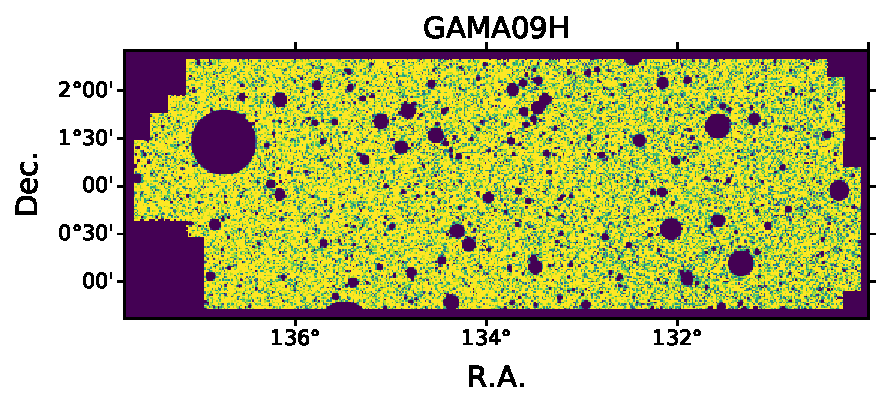
\includegraphics[width=0.49\textwidth]{figures/mask_GAMA09H.pdf}
      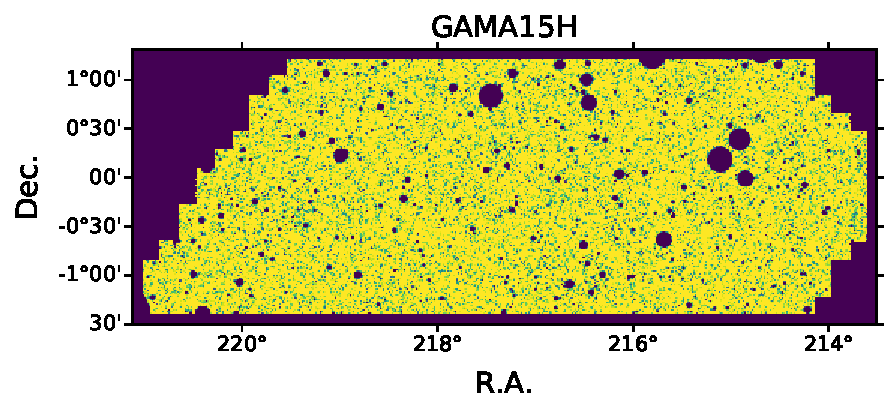
\includegraphics[width=0.49\textwidth]{figures/mask_GAMA15H.pdf}
      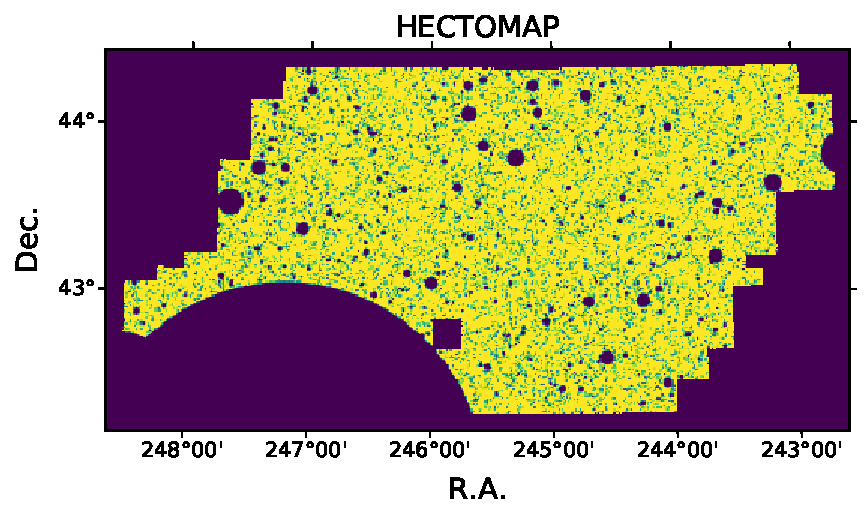
\includegraphics[width=0.49\textwidth]{figures/mask_HECTOMAP.pdf}
      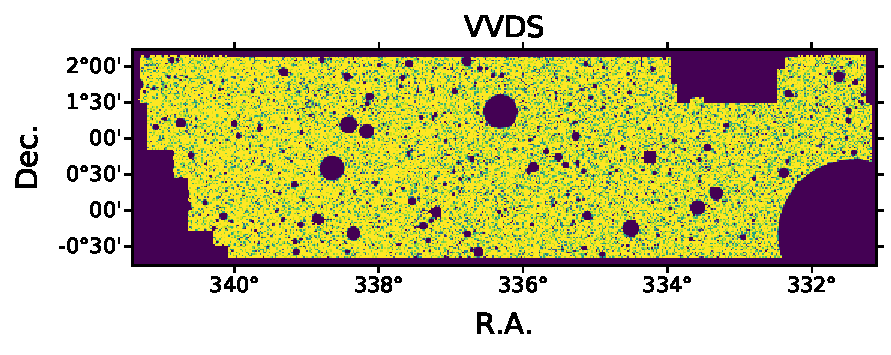
\includegraphics[width=0.49\textwidth]{figures/mask_VVDS.pdf}
      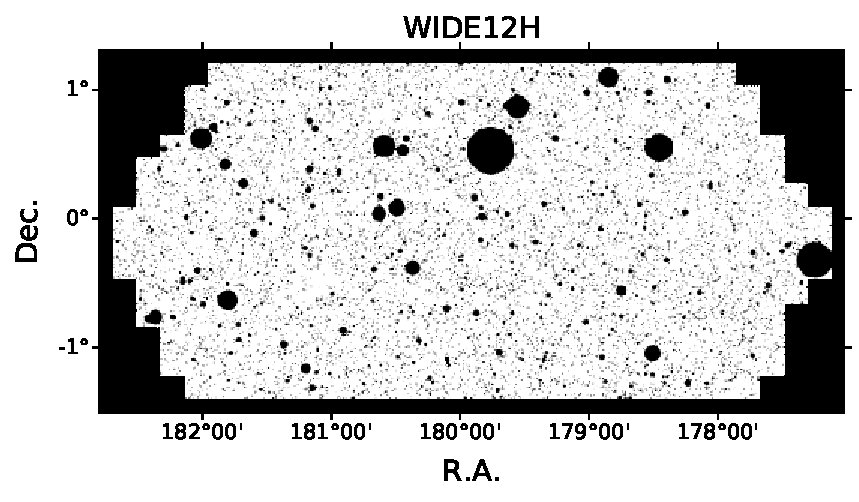
\includegraphics[width=0.49\textwidth]{figures/mask_WIDE12H.pdf}
      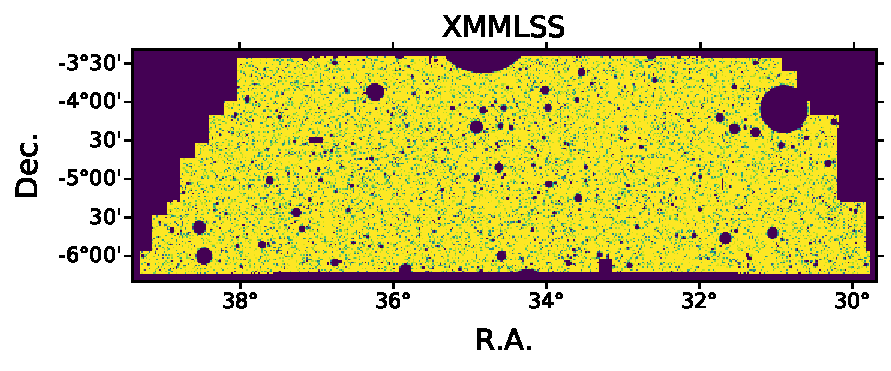
\includegraphics[width=0.49\textwidth]{figures/mask_XMMLSS.pdf}
      \caption{Sky masks for the 6 fields used in this analysis. The map pixels contain values between 0 and 1, corresponding to the fraction of the pixel's area not covered by the fiducial bright-object mask.}
      \label{fig:masks}
    \end{figure}
    The reconstruction of the survey geometry is a central step in order to obtain unbiased estimates of the angular power spectrum. This information is encoded in the so-called ``survey mask'', which minimally contains binary information about which areas of the sky should (mask $=1$) or should not (mask $=0$) be used in the analysis. The basis for our survey mask is the so-called ``bright-object mask'' \cite{2018PASJ...70S...7C}, provided with the HSC DR1, which flags sources that are close to bright stars (mag $<17.5$), with a magnitude-dependent exclusion radius (see \cite{2018PASJ...70S...7C} for details). It is worth noting that the information about the bright object mask is encoded in the HSC DR1 at the catalog level in terms of per-object flags. We transform this information into a pixelized sky map through a multi-step process:
    \begin{enumerate}
      \item We start by creating a low-resolution binary mask based on the presence of objects from the raw catalog in a given pixel. This mask has a pixel size of 0.6 arcmin. The large number density of the raw catalog  ($n_g\sim30\,{\rm arcmin}^{-2}$) is high enough that masked pixels are unlikely to correspond to intrinsically empty regions of the sky, but rather completely unobserved pixels.
      \item We upgrade the low-resolution binary mask to a higher resolution (0.2 arcmin), and remove all pixels containing objects flagged by the bright object mask. We then remove all disconnected, unmasked groups of pixels, corresponding to spurious islands within the exclusion radius of a bright object with no sources in the catalogs.
      \item We downgrade the resulting mask back to the original resolution through an averaging procedure, producing a map quantifying the observed fraction of each pixel.
    \end{enumerate}
    It is worth noting that the resolution of the resulting mask ($0.6$ arcminutes) defines the resolution of all maps used in this analysis. After this procedure, we further mask all pixels with a $10\sigma$ depth below our magnitude limit of $i<24.5$, where the depth is estimated as described in Section \ref{ssec:methods.syst}.

    This defines our fiducial masks, which are shown in Figure \ref{fig:masks} for each field. As part of our systematics analysis (see Section \ref{sssec:results.spectra.syst}), we also study the effect of masking regions with significant contamination from the different observing conditions (described in Section \ref{ssec:methods.syst}) on our measurements. It is worth noting that the NOMAD star catalog \cite{2004AAS...205.4815Z}, one of the datasets used to construct the brigh-object mask described above, is contaminated by a small fraction of bright nearby galaxies ($\sim10\%$). To study the impact of this contamination on our clustering measurements, we have also estimated the angular power spectra using a more recent version of the star mask (the so-called ``Arcturus'' mask described in \cite{2018PASJ...70S...7C}).

  \subsection{Systematics maps}\label{ssec:methods.syst}
    \begin{figure}
      \centering
      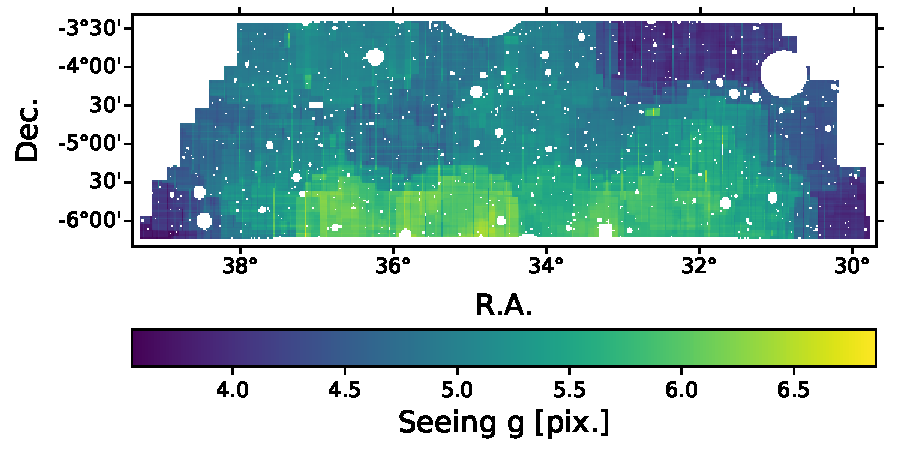
\includegraphics[width=0.49\textwidth]{figures/syst_seeing_g.pdf}
      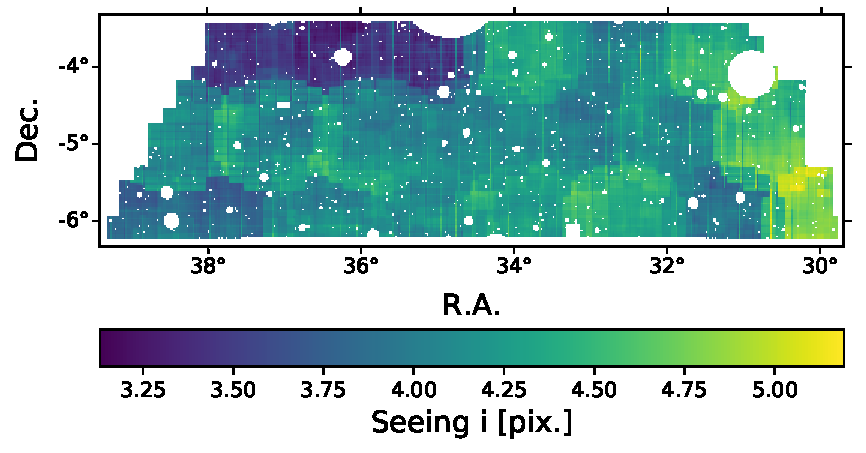
\includegraphics[width=0.49\textwidth]{figures/syst_seeing_i.pdf}
      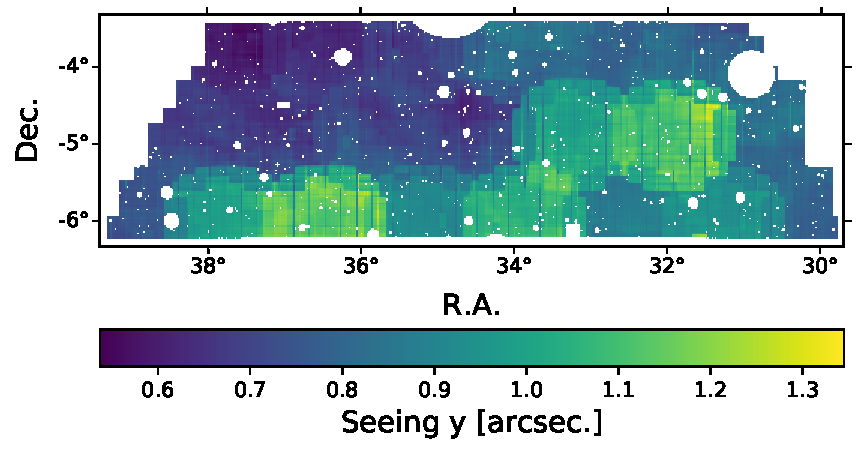
\includegraphics[width=0.49\textwidth]{figures/syst_seeing_y.pdf}
      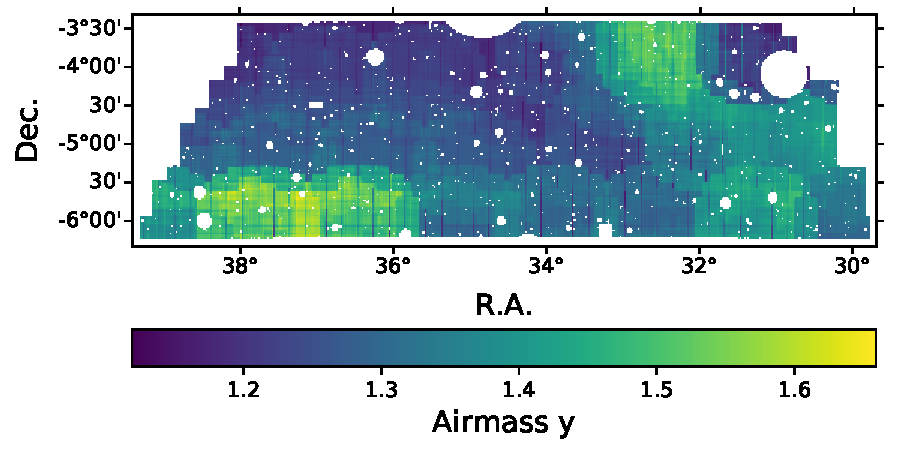
\includegraphics[width=0.49\textwidth]{figures/syst_airmass_y.pdf}
      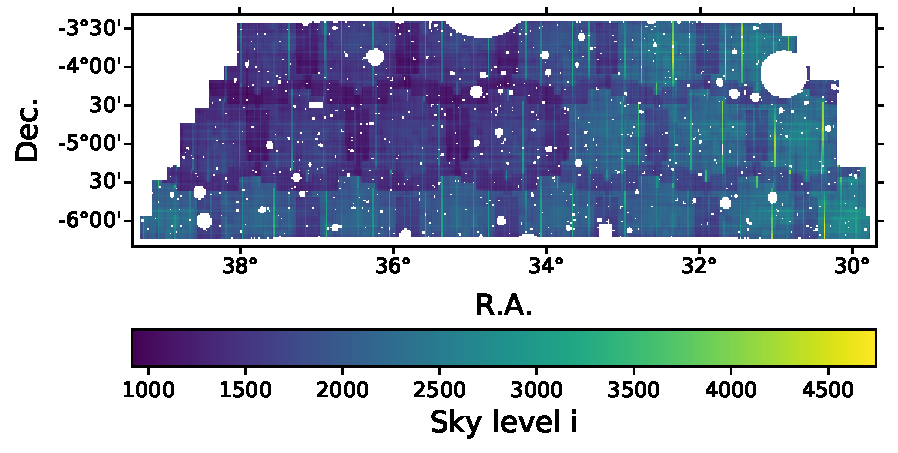
\includegraphics[width=0.49\textwidth]{figures/syst_skylevel_i.pdf}
      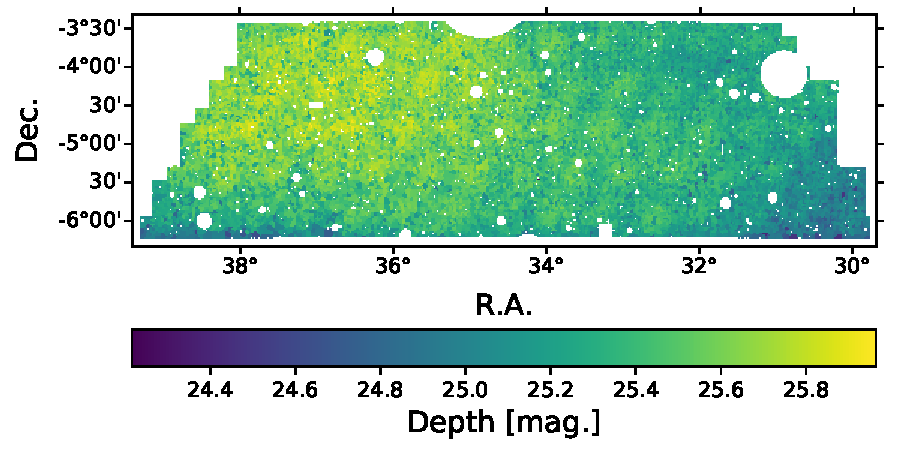
\includegraphics[width=0.49\textwidth]{figures/syst_depth.pdf}
      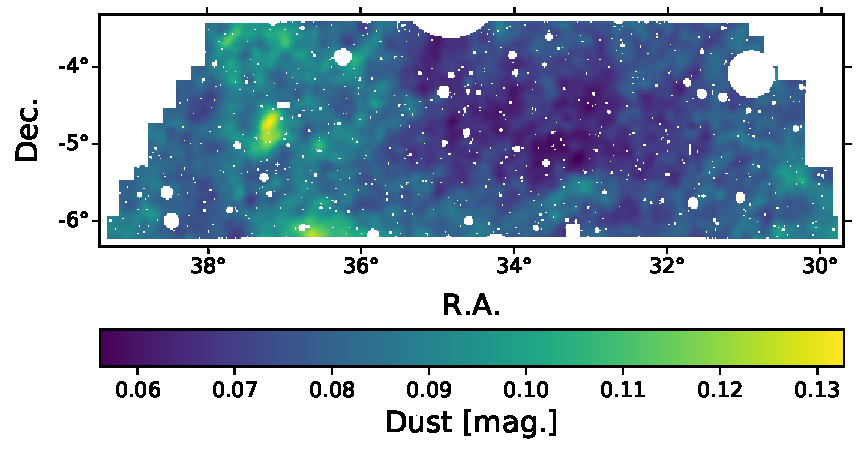
\includegraphics[width=0.49\textwidth]{figures/syst_dust.pdf}
      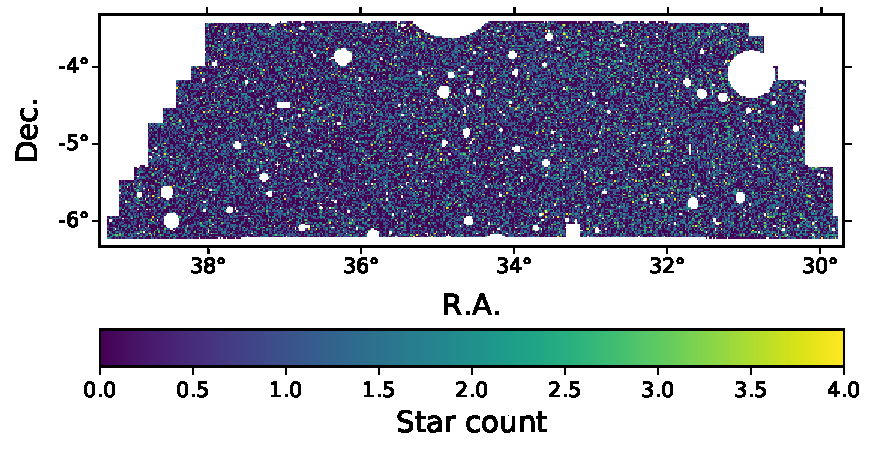
\includegraphics[width=0.49\textwidth]{figures/syst_star.pdf}
      \caption{Maps of different observational systematics that could cause an artificial modulation in the inferred galaxy overdensity. The maps correspond to the XMMLSS field, and were obtained as described in Section \ref{ssec:methods.syst}. From top to bottom and left to right, the different panels show maps of the seeing in the $g$, $i$ and $y$ bands, airmass in the $y$ band, sky level in the $i$ band, $10\sigma$ $i$-band depth, dust absorption and star density. We can visually appreciate the existing correlations between differnt systematics (e.g. seeing and airmass), which are automatically taken into account by the deprojection method described in Section \ref{ssec:methods.cell} and in \cite{2019MNRAS.484.4127A}.}
      \label{fig:sysmap}
    \end{figure}
    A number of astrophysical and observational systematic effects can affect the observed distribution of galaxies, and therefore may bias our inference of their clustering properties. To mitigate this effect we deproject maps of these systematics from our data, as described in Section \ref{ssec:methods.cell}. We generate maps of the most plausible sources of systematic variations in the galaxy number density:
    \begin{enumerate}
      \item {\bf Survey depth}: we estimate the $10\sigma$ survey depth in different directions using a method similar to that outlined in \cite{2018PASJ...70S..25M}. In a given sky pixel, we collect all galaxies with $i$-band {\tt cmodel} fluxes measured with a signal-to-noise ratio between 9 and 11 (i.e. $9\le{\tt icmodel\_flux}/{\tt icmodel\_flux\_err}\le11$), and compute the mean of their $i$-band  {\tt cmodel} magnitude. We verified that we obtain similar depth estimates using other methods (e.g. magnitude corresponding to $10$ times the mean flux error), and that the magnitude limit of our sample ($i<24.5$) is bright enough that little or no area is lost in any of the fields by imposing this cut.
      \item {\bf Dust extinction}: we make maps of dust absorption in each band using the data from \cite{1998ApJ...500..525S} projected onto the 6 HSC DR1 fields.
      \item {\bf Star contamination}: we produce a map of the number density of stars using all objects passing our sample cuts but classified as stars by the star-galaxy separator. As described in Section \ref{ssec:methods.cell}, the method used to remove the impact of this systematic is slightly different from the rest.
      \item {\bf Observing conditions}: the HSC DR1 provides metadata for each filter exposure, containing information about a number of observing conditions. We make coadded maps of these following a procedure similar to that described in \cite{2016ApJS..226...24L}. For each pixel in our map we gather all exposures that fully or partially overlap with it. For each quantity $Q$ in filter $f$, this allows us to build a list of values of $Q$ for each exposure\footnote{It is worth noting that we omit any exposure from CCD 9, since it was found to yield unreliable measurements and was never used in the HSC coadd images.}. We then compute the weighted mean of these values and assign the result to the pixel. The weights used to coadd different exposures consist of the product of the area overlap between pixel and exposure and an approximation of the weights used by the HSC pipeline to produce coadded images \cite{2018PASJ...70S...5B}. Since we do not have direct access to the latter, we used, as coadd weights, the inverse of the sky level of each exposure, which should be close to inverse-variance weighting. Following this procedure we produce maps of the following quantities: airmass, CCD temperature, seeing, point-spread function (PSF) ellipticity, exposure time, sky count level, root-mean square deviation of the sky count and number of visits.
    \end{enumerate}
    Figure \ref{fig:sysmap} shows examples of some of these maps.
    
    Note that an underlying assumption of this step is that the coadded mean of different exposures fully captures the connection between fluctuations in observing conditions and the artificial fluctuations they cause on the number counts. In general we could also consider other cumulants of the per-exposure distribution of observing condition values. As shown below, we do not observe an important contamination from these systematics in our results, and we therefore leave this more thorough study for future work.

  \subsection{Redshift distributions}\label{ssec:methods.nz}
    \begin{figure}
      \centering
      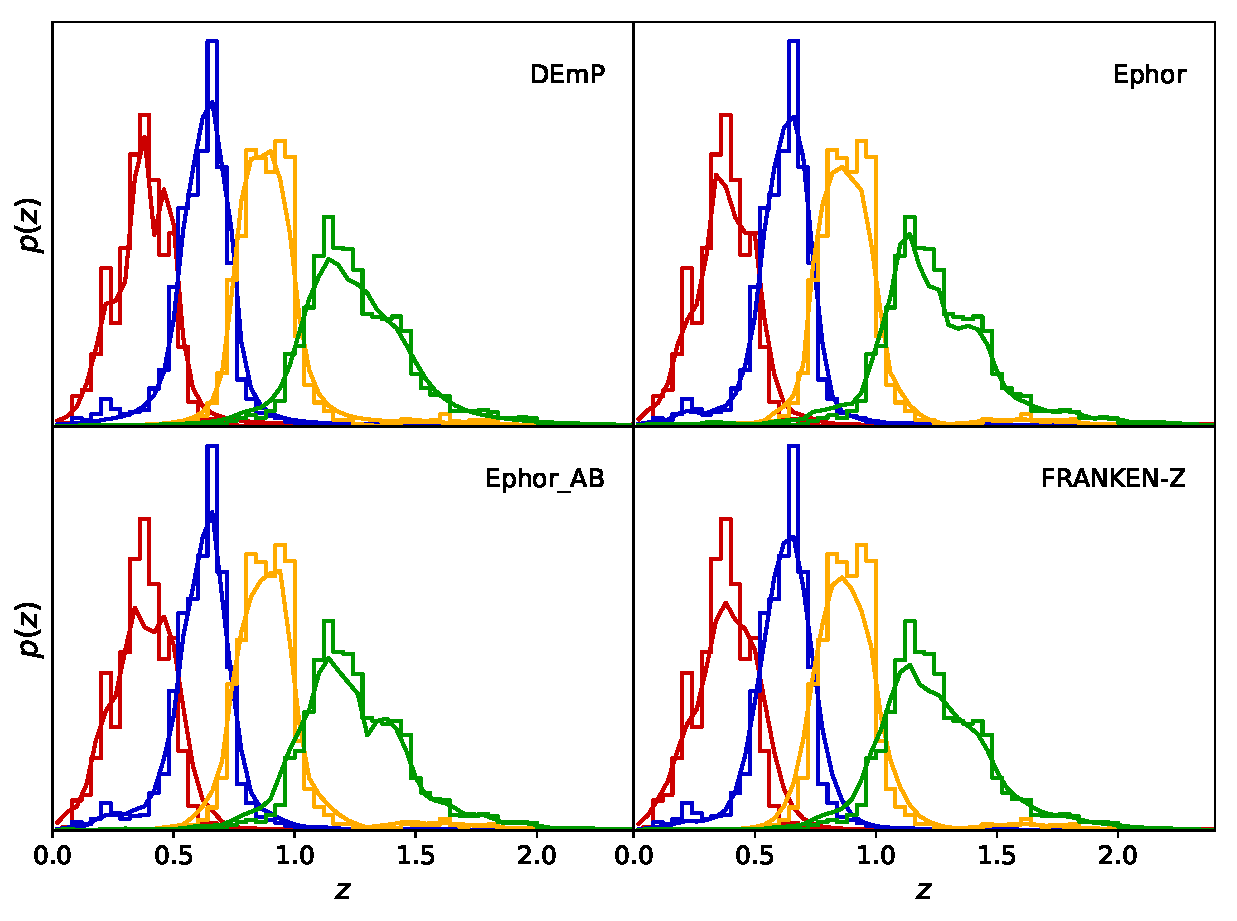
\includegraphics[width=0.9\textwidth]{figures/nzs.pdf}
      \caption{Redshift distributions used in this analysis. The histograms in each panel are the same, and correspond to the redshift distributions estimated from the COSMOS 30-band catalog. These are the fiducial redshift distributions used in our analysis. The solid curves in each panel show the stacked redshift distribution inferred by stacking the per-object photo-$z$ probability distributions obtained with the four alternative photo-$z$ codes explored here ({\tt DEmP}, {\tt Ephor}, {\tt Ephor\_AB} and {\tt Franken-Z} from left to right and top to bottom). The redshift distributions for the four different redshift bins listed in Table \ref{tab:bins_summary} are shown in red, blue orange and green respectively. Note that all four redshift estimation codes use the same COSMOS 30-band catalog so the level of visual agreement should not be taken as realistic measure of uncertainty on the redshift distributions.}
      \label{fig:nzs}
    \end{figure}
    The underlying redshift distributions of our tomographic samples ($p^i(z)$ in Eq. \ref{eq:cell_gg_limber}) are a central component of the theory model used to infer astrophysical and cosmological parameters. Estimating redshift distributions for photometric samples is a non-trivial problem that has been studied extensively in the literature \citep{2008MNRAS.390..118L,2008ApJ...684...88N,2018MNRAS.478..592H}. We use two different methods to estimate $p^i(z)$.
    
    To estimate the fiducial redshift distributions used in our main analysis we make use of the COSMOS 30-band photometric catalog of \cite{2016ApJS..224...24L}. The idea is to use the high-fidelity photo-$z$ estimates in the COSMOS 30-band data as the truth, in which case one can estimate the redshift distribution by simply histogramming these redshifts with appropriate weights. These weights are calculated following the procedure described in \cite{2017MNRAS.465.1454H,2019PASJ...71...43H}, which we summarize here for completeness:
    \begin{enumerate}
      \item We first cross-match all objects in the COSMOS 30-band catalog with sources in the HSC COSMOS field that satisfy our sample cuts (see Section \ref{sec:data}). Matches are found as pairs of objects with an angular separation smaller than 1 arcsecond. All unmached objects in either catalog are discarded.
      \item For each object in the COSMOS 30-band data with a match in HSC, we find its $N_{\rm neigh}^{\rm COSMOS}=20$ nearest neighbours in the COSMOS 30-band sample within the 5-dimensional space of HSC apparent magnitudes $(g,r,i,z,y)$ using a Euclidean metric. We record the distance in this space to the furthest neighbour.
      \item We then compute the number of HSC sources $N_{\rm neigh}^{\rm HSC}$ found within the same radius in magnitude space. The weight applied to the COSMOS 30-band object is then given by the ratio $N^{\rm HSC}_{\rm neigh}/N^{\rm COSMOS}_{\rm neigh}$ normalized by the total number of objects in each sample.
    \end{enumerate}
    There are a number of caveats associated with this method to estimate redshift distributions. First, the COSMOS 30-band photometric redshifts are not as good as a purely spectroscopic sample in terms of redshift accuracy and precision. Second, the small area covered by COSMOS may lead to sample variance uncertainties in the inferred redshift distributions that are difficult to quantify, particularly if the colour-redshift relation has an environmental dependence. Finally, the photo-$z$ codes used in HSC DR1 were trained on the COSMOS 30-band data, which could lead to circularity in the estimation of the redshift distributions.
    
    In order to study the dependence of our results on the method used to estimate the redshift distributions, we have also produced alternative estimates through a stacking approach. In this case, for a given photo-$z$ code, we produce an estimate of the redshift distribution of each tomographic bin by adding the photo-$z$ probability distributions of all objects in that bin. Following this procedure we generate 4 alternative estimates of $p^i(z)$ for the photo-$z$ codes {\tt demp}, {\tt ephor}, {\tt ephor\_ab} and {\tt frankenz} (see \cite{2018PASJ...70S...9T}) \an{HSC gives the pzs from 6 different codes. Should we maybe explain here why we only use 4?.} \da{The only reason is that I had a look at the HSC photo-z paper and it seemed like these ones performed best. We could say that we use a ``representative sample'' of the best-performing photo-z codes?}. The different redshift distributions for all tomographic bins and photo-$z$ methods are shown in Figure \ref{fig:nzs}. The different distributions are visually compatible with each other, although it must be noted that this is, to some extent, by construction, given that the different photo-$z$ codes were trained with the same data from the COSMOS 30-band catalog.

  \subsection{Angular power spectra}\label{ssec:methods.cell}
    We compute angular power spectra using a flat-sky pseudo-$C_\ell$ (PCL) algorithm \citep{2002ApJ...567....2H} as implemented in {\tt NaMaster}\footnote{\url{https://github.com/LSSTDESC/NaMaster}}. The reader is referred to the code's paper \cite{2019MNRAS.484.4127A} for a detailed description of the estimator, but we provide a brief summary here for completeness.
    
    In the absence of a sky mask, the flat-sky auto-power spectrum could be simply estimated Fourier transforming a given map $a_{\bf l}={\rm FT}[a(\nv),{\bf l}]$ (where ${\rm FT}$ denotes a Fourier transform operation, and ${\bf l}$ is a 2D wavenumber), and averaging its modulus squared over bins of $\ell\equiv|{\bf l}|$. In any practical situation, however, it will be desirable to apply weights on the map to e.g. downweight noisy areas or altogether remove pixels that haven't been observed. In this case the observed (``masked'') map is $\tilde{a}(\nv)=w(\nv)a(\nv)$, where $w(\nv)$ is a weight map. The Fourier coefficients of the observed map are therefore given by a convolution of the true Fourier coefficients with the Fourier transform of the mask, coupling different ${\bf l}$ modes in the original map. The result of using the na\"ive estimator of the power spectrum described above on the masked map is therefore a version of the true underlying power spectrum where different $\ell$s are coupled through the so-called {\sl mode-coupling matrix} $M_{\ell\ell'}$:
    \begin{equation}
      \left\langle \tilde{C}^{ab}_\ell \right\rangle = \sum_{\ell'} M_{\ell\ell'}(w_a,w_b)\,C^{ab}_{\ell'}.
    \end{equation}
    Here, $\tilde{C}^{ab}_\ell$ is the power spectrum of two observed fields $\tilde{a}=w_a\,a$ and $\tilde{b}=w_b\,b$, and $C^{ab}_\ell$ is the true power spectrum. As explicitly written above, the mode-coupling matrix depends exclusively on the properties of the survey masks \citep{2002ApJ...567....2H}, and not on the underlying signal maps. The PCL algorithm calculates the mode-coupling matrix analytically using the properties of the weight maps, and uses it to obtain an unbiased estimate of $C^{ab}_\ell$.
    
    The overdensity maps used are constructed as $\delta_{g,p}=N_p/(\bar{N}\,w_p)-1$, where $N_p$ is the number of sources in pixel $p$, $w_p$ is the survey mask described in Section \ref{ssec:methods.mask}, quantifying the unmasked area fraction in each pixel, and $\bar{N}$ is the mean number of sources per pixel, estimated as $\bar{N}=\sum_p N_p/\sum_p w_p$.
    
    An important aspect of power spectrum estimation that is particularly relevant for galaxy clustering studies is accounting for the effect of sky contaminants on the final summary statistic. In this analysis we have done so using a technique called ``template deprojection''. We start by compiling a list of maps of quantities that can potentially cause artificial perturbations in the observed number density of sources. These include all the quantities described in Section \ref{ssec:methods.syst}.
    
    For small levels of contamination, we can start by assuming that these contaminants affect the observed galaxy overdensity at a linear level:
    \begin{equation}\label{eq:deproj1}
      \delta_g^{\rm obs}(\nv) = \delta_g^{\rm true}(\nv) + A_{\rm syst}\,\Delta_{\rm syst}(\nv),
    \end{equation}
    where $\Delta_{\rm syst}$ is a template map of the fluctuation of a given contaminant around its mean across the survey footprint, and $A_{\rm syst}$ is an unknown linear factor. Template deprojection methods avoid systematic biases by removing all modes from the observed maps that are common to any of the systematic template maps, effectively projecting the input map onto the subspace that is orthogonal to all the contaminant templates. This is equivalent to building a Gaussian model for the observed map using Equation \ref{eq:deproj1} and marginalizing over the free amplitude $A_{\rm sys}$. In the context of pseudo-$C_\ell$ estimators this is achieved in practice by obtaining the best-fit value of $A_{\rm syst}$, subtracting the corresponding best-fit contaminant contribution from the maps and analytically accounting for the associated loss of modes when computing the angular power spectrum. Further details of this method can be found in \cite{2017MNRAS.465.1847E,2019MNRAS.484.4127A}.
    
    We must note that star contamination is a special type of contaminant, since it is an additive contribution to the observed galaxy number density $n_g$, not its overdensity. In the simplest scenario, a fraction $f$ of stars contribute to the observed galaxy density: $n_g^{\rm obs}=n^{\rm true}_g+f\,n_s$, where $n_s$ is the local number density of stars. A fluctuation in the star density around the mean $\Delta_s(\nv)=n_s(\nv)/\bar{n}_s-1$, therefore produces both a multiplicative and an additive effect on $\delta_g$:
    \begin{equation}
      \delta_g^{\rm obs}(\nv) = (1-F_s)\,\delta_g^{\rm true}(\nv)+F_s\,\Delta_s(\nv),
    \end{equation}
    where $F_s$ is the fraction of the sample made out of stars (i.e. $F_s\equiv f\bar{n}_s/(\bar{n}_g+f\bar{n}_s)$ with the notation above). The linear term is taken care of by the deprojection procedure, and we correct the final map of $\delta_g$ by a factor $1/(1-F_s)$, where we estimate $F_s\simeq0.02$ independent of redshift from the HSC deep COSMOS field. This estimate is consistent with the star contamination found in the HSC DR1 shape catalog \citep{2018PASJ...70S..25M}.

    As noted above, the power spectra are computed in rings of $\ell=|{\bf l}|$, which we will call bandpowers here. We use 17 contiguous bandpowers with edges $\ell=$(100, 200, 300, 400, 600, 800, 1000, 1400, 1800, 2200, 3000, 3800, 4600, 6200, 7800, 9400, 12600, 158800). Due to this bandpower averaging, the estimated power spectra cannot, strictly speaking, be compared with theoretical predictions estimated at token multipoles (e.g. the midpoint of each band). The effect of this averaging can however be taken into account exactly as a linear operation of the form $\bar{C}_b=\sum_\ell F^b_{\ell} C_\ell$, where $C_\ell$ is the theoretical prediction evaluated at all integer multipoles $\ell$, $\bar{C}_b$ is the prediction for the $b$-th bandpower and the bandpower windows $F^b_{\ell}$ incorporate the effects of mode-coupling, averaging into bandpowers and the inversion of the binned mode-coupling matrix.
    
    Finally, a noise bias term must be subtracted from all auto-power spectra. In the case of galaxy clustering, and assuming this noise is entirely due to Poisson shot noise, this can be done analytically as described in \cite{2019MNRAS.484.4127A}. In short, the noise power spectrum before mode-decoupling (i.e. before multiplying by the inverse mode-coupling matrix), can be calculated as:
    \begin{equation}\label{eq:nell}
      \tilde{N}_\ell = \Omega_{\rm pix}\,\frac{\bar{w}}{\bar{N}},
    \end{equation}
    where $\bar{w}$ is the mean value of the survey mask across the map, $\bar{N}$ is the mean number density of sources per pixel, and $\Omega_{\rm pix}$ is the pixel area in units of steradians.

  \subsection{Modelling the signal}\label{ssec:methods.theory}
  \subsubsection{Projected quantities and power spectra}\label{sssec:methods.theory.cellpk}
    Our main observable is the projected overdensity of galaxies $\delta^i_g(\nv)$ as a function of sky position $\nv$ in a given redshift bin labelled by $i$. This is related to the 3D galaxy overdensity $\Delta_g$ through
    \begin{equation}
      \delta^i_g(\nv)=\int \mathrm{d}z\,p^i(z)\,\Delta_g\left(t(z),\chi(z)\nv\right).
    \end{equation}
    Here $t(z)$ and $\chi(z)$ are the cosmic time and radial comoving distance as a function of redshift, and $p^i(z)$ is the redshift bin window function, given by the true redshift distribution of objects in the bin normalized to unit area.
  
    Given the small size of the sky patches covered by the HSC DR1, we will adopt the flat sky approximation for simplicity, in which case $\nv$ is a 2D vector. It is common to decompose $\delta^i_g(\nv)$ into its Fourier coefficients
    \begin{equation}
      a^i_{\bf l}\equiv \int\frac{\mathrm{d}\theta^2}{2\pi}e^{-i{\bf l}\cdot\nv}\delta^i_g(\nv).
    \end{equation}
    The variance of the Fourier coefficients is the so-called angular power spectrum $\langle a^i_{\bf l}a^{j*}_{{\bf l}'}\rangle = C^{ij}_\ell\,\delta^{\cal D}({\bf l}-{\bf l}')$, where $\delta^{\cal D}$ is the 2D Dirac delta function. The 3D power spectrum $P_{gg}(z,{\bf k})$ is defined analogously for the 3D Fourier coefficients of $\Delta_g$. Both quantities are related to each other through:
    \begin{equation}\label{eq:cell_gg_limber}
      C^{ij}_\ell = \int \mathrm{d}z\,\frac{H(z)}{\chi^2(z)} p^i(z)p^j(z)\,P_{gg}\left(z,k=\frac{\ell+1/2}{\chi(z)}\right),
    \end{equation}
    where $H(z)$ is the expansion rate at redshift $z$, and we have used the so-called Limber approximation\footnote{We note that we have compared the power spectra for the redshift distributions employed in this work obtained with the Limber approximation and those obtained making no approximations. We find the results to be virtually the same and in the following we therefore use the Limber approximation to compute projected power spectra for computational speed.} \citep{Limber:1953, Kaiser:1992, Kaiser:1998}.

  \subsubsection{Halo Occupation Distribution}\label{sssec:methods.theory.hod}
    In order to model $P_{gg}(z,k)$ we use a halo occupation distribution (HOD) model \citep{2000MNRAS.318.1144P,2002PhR...372....1C,2002ApJ...575..587B,2005ApJ...633..791Z,2013MNRAS.430..725V}. In this halo model-based prescription we model the galaxy content of dark matter haloes as a function of halo mass. Details about HOD parametrizations can be found in \cite{2011ApJ...736...59Z}. In short, the galaxy power spectrum receives contributions from the so-called 1-halo and 2-halo terms:
    \begin{equation}
      P_{gg}(z,k) = P_{gg,{\rm 1h}}(z,k) + P_{gg,{\rm 2h}}(z,k),
    \end{equation}
    where
    \begin{align}
      & P_{gg,{\rm 1h}}(k)=\frac{1}{\bar{n}_g^2} \int \mathrm{d}M\,\frac{\mathrm{d}n}{\mathrm{d}M} \bar{N}_c\,\left[\bar{N}_s^2u_s^2(k)+2\bar{N}_su_s^2(k)\right],\\
      & P_{gg,{\rm 2h}}(k)=\left(\frac{1}{\bar{n}_g} \int \mathrm{d}M\,\frac{\mathrm{d}n}{\mathrm{d}M}\,b_h(M)\,\bar{N}_c\,\left[1+\bar{N}_su_s(k)\right]\right)^2\,P_{\rm lin}(k).
    \end{align}
    Here, $M$ represents halo mass, $\sfrac{\mathrm{d}n}{\mathrm{d}M}$ is the halo mass function, $b_h(M)$ is the halo bias, $\bar{N}_c(M)$ and $\bar{N}_s(M)$ are the mean number of central and satellite galaxies respectively, $u_s(k)$ is the Fourier transform of the normalized density profile of satellite galaxies, $P_{\rm lin}(k)$ is the linear matter power spectrum and $\bar{n}_g$ is the total mean galaxy density, given by
    \begin{equation}
      \bar{n}_g=\int \mathrm{d}M\,\frac{\mathrm{d}n}{\mathrm{d}M}\bar{N}_c(M)\left[1+\bar{N}_s(M)\right].
      \label{eq:ng_hod}
    \end{equation}
    A central assumption in standard HOD parametrizations is that centrals/satellites follow a binomial/Poisson distribution.

    Following \cite{2011ApJ...736...59Z}, we parametrise the number of centrals and satellites as a function of mass as:
    \begin{align}
      &\bar{N}_c(M)=\frac{1}{2}\left[1+{\rm erf}\left(\frac{\log(M/M_{\rm min})}{\sigma_{{\rm ln}M}}\right)\right],\\
      &\bar{N}_s(M)=\Theta(M-M_0)\left(\frac{M-M_0}{M_1'}\right)^\alpha,
    \end{align}
    where $\Theta(x)$ is the Heavyside step function. Furthermore, we assume that $N_c$ follows a Bernoulli distribution with probability $p=\bar{N}_c$, and that the number of satellites is Poisson-distributed with mean $\bar{N}_s$. Finally, we model the distribution of satellites to follow that of the dark matter, and therefore $u_s$ is a Navarro-Frenk-White profile, given by:
    \begin{equation}
      u_s(k|M)=\frac{\sin x\left[{\rm Si}\left((1+c)\,x\right)-{\rm Si}(x)\right]+\cos x\left[{\rm Ci}\left((1+c)x\right)-{\rm Ci}(x)\right]-\frac{\sin(cx)}{(1+c)x}}{{\rm ln}(1+c)-\frac{c}{1+c}},
    \end{equation}
    where $x=\sfrac{k R_\Delta}{c}$, $R_\Delta$ is the halo radius, $c=c(M)$ is the concentration parameter, and ${\rm Si}/{\rm Ci}$ are the sine and cosine integral functions. We define $R_\Delta$ as the radius that encloses $\Delta=200$ times the background matter density. The concentration-mass relation $c(M)$ also depends on the choice of $\Delta$, and we follow the parametrization of \cite{Duffy:2008}. In this work, we model the halo mass function $\sfrac{\mathrm{d}n}{\mathrm{d}M}$ following \cite{Tinker:2010}. Furthermore, we employ the concentration-mass relation $c(M)$ (which depends on the choice of $\Delta$) derived by \cite{Duffy:2008}.

    In order to include lensing magnification in the theory prediction (see Section \ref{ssec:results.magnification}), we also need to model the galaxy-matter and matter-matter power spectra (see Eq. \ref{eq:cell_gg_wmag}). Following the HOD parametrization, the 1-halo and 2-halo contributions to $P_{gm}(k)$ are given by:
    \begin{align}
      & P_{gm,{\rm 1h}}(k)=\frac{1}{\bar{n}_g\bar{\rho}_M} \int \mathrm{d}M\,\frac{\mathrm{d}n}{\mathrm{d}M} M\,\bar{N}_c\,\left[1+\bar{N}_su_s(k)\right],\\
      & P_{gm,{\rm 2h}}(k)=\left(\frac{1}{\bar{n}_g} \int \mathrm{d}M\,\frac{\mathrm{d}n}{\mathrm{d}M}\,b_h(M)\,\bar{N}_c\,\left[1+\bar{N}_su_s(k)\right]\right)\,P_{\rm lin}(k),
    \end{align}
    where $\bar{\rho}_M$ is the comoving matter density. $P_{mm}(k)$ is given by the {\tt Halofit} fitting function \cite{Smith:2003} with the revisions of \cite{Takahashi:2012}.

    It is a well-known fact that the simple halo model implementation described here is not able to accurately describe the ``quasi-linear'' scales in the transition between the 1-halo and 2-halo-dominated regimes, corresponding to $k\sim0.1\,{\rm Mpc}^{-1}$ at $z\sim0$ \citep{2015MNRAS.454.1958M}. To correct for this inaccuracy, we multiply $P_{gg}$ and $P_{gm}$ by a universal scale-dependent factor, given by the ratio between the {\tt Halofit} and the pure halo model predictions for $P_{mm}$:
    \begin{equation}
      R(z,k)=\frac{P^{\rm Halofit}_{mm}(z,k)}{P^{\rm halo\,model}_{mm}(z,k)},
    \end{equation}
 which we compute for our fiducial cosmological model given in Sec.~\ref{ssec:methods.constr}.
 
    We expect mean galaxy properties to evolve as a function of redshift for the magnitude-limited sample considered in this analysis. Instead of fitting a separate HOD model to each redshift bin, we fit redshift-dependent functions to $M_{\mathrm{min}}(z)$, $M_{0}(z)$ and $M_{1}(z)$ and choose a functional form given by:
    \begin{equation}
      \log{M_{i}(z)} = M_{i} + M_{i, p} \left(\frac{1}{1+z} - \frac{1}{1+z_{p}}\right),
    \end{equation}
    where $\log$ is the logarithm to base 10, $i \in [\mathrm{min}, 0, 1]$ and $z_{p}$ denotes a pivot redshift, which we set to $z_{p} = 0.65$. This functional form is motivated by an initial analysis in which we separately fit an HOD to each auto power spectrum and determine a function consistent with the observed redshift evolution of the three parameters $M_{\mathrm{min}}(z)$, $M_{0}(z)$ and $M_{1}(z)$. We additionally include a pivot redshift $z_{p}$ in our parametrization to remove degeneracies between the fitted parameters.

\subsubsection{Photometric redshift systematics modeling}\label{sssec:methods.theory.photoz_syst}

Uncertainties in photometric redshifts (photo-$z$) represent one of the major systematics in photometric galaxy clustering analyses. To lowest order, errors in photo-$z$'s cause shifts in the means and changes in the width of the derived redshift distribution for a population of galaxies. In this work, we therefore choose to parametrize the impact of photo-$z$ errors on the derived galaxy redshift distributions $p_{i}(z)$ using a two-parameter model given by
\begin{equation}
p_{i}(z) = \hat{p}_{i}(z_{c} + (1 + z_{w, i})(z-z_{c}) + \Delta z_{i}),
\label{eq:photo-z-model}
\end{equation} 
where the index $i$ runs over the number of redshift bins considered in our analysis.
In the above equation, $\hat{p}(z)$ denotes the estimated redshift distribution while $p(z)$ is the underlying true distribution. The parameters $\Delta z_{i}$ account for shifts in the means of the distributions and changes to their widths are parameterized through $z_{w, i}$. The quantity $z_{c}$ is kept constant in our analysis and is set to the redshift at which $\hat{p}(z)$ attains its maximal value.
    
  \subsubsection{Covariance matrices}\label{sssec:methods.theory.covar}
    We use an analytical procedure to estimate the uncertainties of our measured power spectra, inspired in the methods used by \cite{Krause:2017}. As shown in \cite{2009MNRAS.395.2065T,Takada:2013}, the covariance matrix for large-scale structure data can be decomposed into a disconnected trispectrum part, essentially equivalent to the covariance of a Gaussian random field with the same power spectrum as the data, a connected part, caused by the non-Gaussian nature of the density field, and a super-sample covariance term (labelled SSC here). The SSC contribution accounts for the coherent shift in the amplitude of density fluctuations within the surveyed volume caused by long wavelength modes larger than the survey.
    
    We estimate the Gaussian covariance of the pseudo-$C_\ell$ estimator as described in \cite{2004MNRAS.349..603E,2019arXiv190611765G}. In the absence of any approximations, the covariance of the observed power spectra is given by
    \begin{equation}
      {\rm Cov}\left(\tilde{C}^{ab}_\ell,\tilde{C}^{cd}_{\ell'}\right)=\sum_{{\bf l}_1,{\bf l}_2} C^{ac}_{\ell_1}C^{bd}_{\ell_2}W^a_{{\bf l}{\bf l}_1}W^b_{{\bf l}{\bf l}_2}W^c_{{\bf l}'{\bf l}_1}W^d_{{\bf l}'{\bf l}_2} + C^{ad}_{\ell_1}C^{bc}_{\ell_2}W^a_{{\bf l}{\bf l}_1}W^b_{{\bf l}{\bf l}_2}W^c_{{\bf l}'{\bf l}_2}W^d_{{\bf l}'{\bf l}_1},
    \end{equation}
    where $W^x_{{\bf l}{\bf l}'}$ are coupling coefficients depending only on the mask of $x$ (see \cite{2019arXiv190611765G} for further details). In the absence of further approximations, computing the covariance matrix would therefore imply solving a 4-dimensional integral for each pair $(\ell,\ell')$. This is an $O(\ell_{\rm max}^6)$ operation which easily becomes computationally unfeasible. Since the coupling coefficients $W^x_{{\bf l}{\bf l}'}$ are usually highly peaked around ${\bf l}={\bf l}'$, we can proceed further by approximating the power spectra to be constant within the support of $W^x_{{\bf l},{\bf l}'}$. Effectively this implies approximating
    \begin{equation}
      C^{ac}_{\ell_1}C^{bd}_{\ell_2}\simeq C^{ac}_{(\ell}C^{bd}_{\ell')}\equiv\frac{1}{2}\left(C^{ac}_\ell C^{bd}_{\ell'}+C^{ac}_{\ell'} C^{bd}_\ell\right).
    \end{equation}
    This allows us to simplify the expression above significantly, leading to
    \begin{equation}
      {\rm Cov}\left(\tilde{C}^{ab}_\ell,\tilde{C}^{cd}_{\ell'}\right)=(2\ell'+1)^{-1}\left[C^{ac}_{(\ell}C^{bd}_{\ell')}M_{\ell\ell'}(w_aw_c,w_bw_d)+C^{ad}_{(\ell}C^{bc}_{\ell')}M_{\ell\ell'}(w_aw_d,w_bw_c)\right].
    \end{equation}

    Where $M_{\ell\ell'}$ are the mode-coupling matrices described in the previous section, except now they are computed from the products of two masks. It has been shown by \cite{2019arXiv190611765G} that this approach yields a very good approximation for the power spectrum covariance, fully accounting for the effects of mode coupling due to survey geometry.

    The second contribution to the total covariance matrix for galaxy clustering is caused by the connected part of the trispectrum, which accounts for mode-coupling due to the non-Gaussian nature of the density field. In our work we estimate this contribution using the halo model coupled with a halo occupation distribution. In general, this contribution is given by the angular projection of the three-dimensional trispectrum as (see e.g. \cite{Krause:2017}) \todo{Also, you need to define the $q$s.}
    \begin{equation}
    \begin{aligned}
      \mathrm{Cov}_{\mathrm{NG}}(C^{ab}_{\ell}, C^{cd}_{\ell'}) = \frac{1}{4 \pi f_{\mathrm{sky}}} \int_{\vert \boldsymbol{\ell} \vert \in \ell_{1}} \int_{\vert \boldsymbol{\ell}' \vert \in \ell_{2}} \int \frac{\mathrm{d}^{2}\boldsymbol{\ell}}{A(\ell_{1})} \; \frac{\mathrm{d}^{2}\boldsymbol{\ell}'}{A(\ell_{2})} \; \mathrm{d}\chi \; \frac{q^{a}(\chi)q^{b}(\chi)q^{c}(\chi)q^{d}(\chi)}{\chi^{6}} \times \\ T^{abcd}(\sfrac{\boldsymbol{\ell}}{\chi}, \sfrac{-\boldsymbol{\ell}}{\chi}, \sfrac{\boldsymbol{\ell}'}{\chi}, \sfrac{-\boldsymbol{\ell}'}{\chi}).
    \end{aligned}
    \end{equation}
    The quantity $A(\ell_{i})$ denotes the area of an annulus of width $\Delta \ell_{i}$ around $\ell_{i}$, i.e. $A(\ell_{i}) = \int_{\vert \boldsymbol{\ell} \vert \in \ell_{i}} \mathrm{d}^{2}\boldsymbol{\ell}$, which is approximately given by $A(\ell_{i}) \approx 2 \pi \Delta \ell_{i} \ell_{i}$ for $\ell_{i} \gg \Delta \ell_{i}$.
    
    Using the halo model, the connected part of the trispectrum $T^{abcd}$ can be written as (e.g. \cite{Takada:2013}):
    \begin{equation}
      T^{abcd} = T^{abcd, 1h} + (T^{abcd, 2h}_{22} + T^{abcd, 2h}_{13}) + T^{abcd, 3h} + T^{abcd, 4h},
    \end{equation}
    where
    \begin{align}
      &T^{abcd, 1h}(\mathbf{k}_{a}, \mathbf{k}_{b}, \mathbf{k}_{c}, \mathbf{k}_{d}) = I^{0}_{abcd}(k_{a}, k_{b}, k_{c}, k_{d}), \\
      &T^{abcd, 2h}_{22}(\mathbf{k}_{a}, \mathbf{k}_{b}, \mathbf{k}_{c}, \mathbf{k}_{d}) = P_{\mathrm{lin}}(k_{ab})I^{1}_{ab}(k_{a}, k_{b})I^{1}_{cd}(k_{c}, k_{d}) + 2 \; \mathrm{perm.}, \\
      &T^{abcd, 2h}_{13}(\mathbf{k}_{a}, \mathbf{k}_{b}, \mathbf{k}_{c}, \mathbf{k}_{d}) = P_{\mathrm{lin}}(k_{a})I^{1}_{a}(k_{a})I^{1}_{bcd}(k_{b}, k_{b}, k_{c}) + 3 \; \mathrm{perm.}, \\
      &T^{abcd, 3h}(\mathbf{k}_{a}, \mathbf{k}_{b}, \mathbf{k}_{c}, \mathbf{k}_{d}) = B^{\mathrm{PT}}(\mathbf{k}_{a}, \mathbf{k}_{b}, \mathbf{k}_{cd})I^{1}_{a}(k_{a})I^{1}_{b}(k_{b})I^{1}_{cd}(k_{c}, k_{d}) + 5 \; \mathrm{perm.},\\
      &T^{abcd, 4h}(\mathbf{k}_{a}, \mathbf{k}_{b}, \mathbf{k}_{c}, \mathbf{k}_{d}) = T^{\mathrm{PT}}(\mathbf{k}_{a}, \mathbf{k}_{b}, \mathbf{k}_{c}, \mathbf{k}_{d})I^{1}_{a}(k_{a})I^{1}_{b}(k_{b})I^{1}_{c}(k_{c})I^{1}_{d}(k_{d}).
    \label{eq:halo-mod-trisp}
    \end{align}
    Here, ${\bf k}_{ab}\equiv {\bf k}_a+{\bf k}_b$, and the quantities $B^{\mathrm{PT}}$ and $T^{\mathrm{PT}}$ denote the matter bi- and trispectrum respectively, as estimated using tree-level perturbation theory. The full expressions for these terms can be found in \cite{Takada:2013}. Finally, $I^{n}_{a_1...b_m}$ denotes the generic halo model integral, defined as (e.g. \cite{Krause:2017}):
    \begin{equation}
      I^{n}_{a_1...a_m}(k_1,...,k_m) = \int \mathrm{d}M \frac{\mathrm{d}n}{\mathrm{d}M}b_{h, n}(M)  \left\langle\prod_{i=1}^m \left[\tilde{u}_{a_i}(k_i, M) \right]\right\rangle, \\
    \end{equation}
    where $b_{h,1}(M)\equiv b_h(M)$ is the halo bias, $b_{h,0}\equiv1$, and $\tilde{u}_{a_i}$ is the halo profile for the $i$-th field being correlated (e.g. the HOD profile described in Section \ref{sssec:methods.theory.hod} in the case of galaxy clustering). For simplicity, we follow \cite{Krause:2017} and approximate the 2- to 4-halo trispectrum as the linearily biased matter trispectrum and only include a probe-specific 1-halo trispectrum contribution. Specifically, we set 
    \begin{equation}
      T^{abcd} = T^{abcd, 1h} + b_{a}b_{b}b_{c}b_{d}T^{m, 2h+3h+4h},
    \end{equation}
where $T^{abcd, 1h}$ and $T^{m, 2h+3h+4h}$ are computed following Equations \ref{eq:halo-mod-trisp} and $b_{i}$ denotes the linear bias predicted using halo occupation distribution modeling, given by
    \begin{equation}
      b_{a}=\frac{1}{\bar{n}_{g, a}}\int \mathrm{d}M\,\frac{\mathrm{d}n}{\mathrm{d}M}b_{h}(M) \bar{N}_{c, a}(1+\bar{N}_{s, a}).
    \end{equation}
    The 1-halo trispectrum $T^{abcd, 1h}$ for galaxies also receives contributions due to shot noise \cite{Lacasa:2018}. However, these are expected to be small \cite{Lacasa:2018} and we thus neglect them in this work.

    Finally, we compute the super-sample covariance contribution following the treatment of \cite{Krause:2017}, i.e.:
    \begin{align}
       \mathrm{Cov}_{\mathrm{SSC}}(C^{ab}_{\ell}, C^{cd}_{\ell'}) &= \int \mathrm{d}\chi \;\frac{q^{a}(\chi)q^{b}(\chi)q^{c}(\chi)q^{d}(\chi)}{\chi^{4}} \times \\ &\frac{\partial P_{ab}(\sfrac{\ell}{\chi}, z(\chi))}{\partial \delta_{\rm LS}}\frac{\partial P_{cd}(\sfrac{\ell'}{\chi}, z(\chi))}{\partial \delta_{\rm LS}}\sigma^{2}_{b}(z(\chi)).
    \end{align}
        The quantity $\sigma_b^2(z)$ is the variance of the long wavelength mode $\delta_{\rm LS}$ over the survey footprint, given by
    \begin{equation}
      \sigma_b^2(z) = \int \frac{\mathrm{d}k_\perp^2}{(2\pi)^2}P_{\rm lin}(k_\perp,z)\left|W(k_\perp,z)\right|^2.
    \end{equation}
    Furthermore $W(k_\perp,z)$ denotes the Fourier transform of the survey footprint, which we approximate as a compact circle with an area matched to our data set:
    \begin{equation}
      W(k_\perp,z)=\frac{2 J_1(k_\perp\chi(z)\theta_s)}{k_\perp \chi(z)\theta_s},\hspace{12pt} \theta_s={\rm arccos}(1-2f_{\rm sky}),
    \end{equation}
    where $J_1(x)$ is the cylindrical Bessel function of order 1.
    Finally, the quantity $\partial P_{ab}(k, z)/\partial \delta_{\rm LS}$ is the response of the power spectrum $P_{ab}$ to a large-scale density fluctuation, which we estimate using the halo model and results from perturbation theory as (e.g. \cite{Krause:2017}):
    \begin{align}
      \frac{\partial P_{ab}(k, z)}{\partial \delta_{\rm LS}} &= \left( \frac{68}{21} - \frac{1}{3}\frac{\mathrm{d}\log{k^{3} P_{\mathrm{lin}}}(k, z)}{\mathrm{d}\log k} \right) I_{a}^{1}(k)I_{b}^{1}(k)P_{\mathrm{lin}}(k, z) + I_{ab}^{1}(k, k) \\ &- (b_{a} + b_{b})P_{ab}(k, z).
    \label{eq:ps-resp}  
    \end{align}
The last term in Eq.~\ref{eq:ps-resp} accounts for the fact that the observed galaxy overdensity is computed using the mean galaxy density estimated inside the survey volume.
    
For consistency with our implementation of the trispectrum, we compute the response function $\sfrac{\partial P_{ab}(k, z)}{\partial \delta_{\rm LS}} $ for a given probe as the linearly biased response of the matter field\footnote{In order to test the robustness of our results to this approximation, we also compute the SSC contribution to the covariance using the probe-specific halo model quantities in Eq.~\ref{eq:ps-resp}. We find our parameter constraints to be unaffected by this change and therefore resort to the approach described above for consistency.}. 

  \subsection{Parameter constraints}\label{ssec:methods.constr}
    In order to derive constraints on HOD, cosmological and systematics parameters, we assume the joint likelihood of all auto- and cross power spectra to be Gaussian 
    \begin{align}
      \mathscr{L}(D \vert \theta) = \frac{1}{[(2\pi)^{d}\det{\mathsf{C}}]^{\sfrac{1}{2}}} e^{-\frac{1}{2}(\mathbf{C}^{\mathrm{obs}}_{\ell}-\mathbf{C}^{\mathrm{theor}}_{\ell})^{\mathrm{T}}\mathsf{C}^{-1}(\mathbf{C}^{\mathrm{obs}}_{\ell}-\mathbf{C}^{\mathrm{theor}}_{\ell})}.
      \label{eq:likelihood}
    \end{align}
    The quantity $\mathsf{C}$ denotes the joint covariance matrix, which we estimate analytically as described in Sec.~\ref{sssec:methods.theory.covar} and is kept constant during parameter estimation \citep{2019OJAp....2E...3K}.
    We sample the likelihood in a Monte Carlo Markov Chain (MCMC) using the publicly available code \texttt{CosmoHammer} \cite{Akeret:2013}, which is based on \texttt{emcee} \cite{Foreman-Mackey2013}\footnote{We note that we have compared the MCMC results obtained using \texttt{CosmoHammer} to those obtained using a Metropolis-Hastings algorithm as implemented in \texttt{april} (https://github.com/slosar/april), finding consistent results for our test case.}. In our fiducial analysis we sample the parameter set $\boldsymbol{\theta} = \{M_{\mathrm{min}}, \allowbreak \, M_{\mathrm{min}, p}, \allowbreak \, M_{0}, \allowbreak \, M_{0, p}, \allowbreak \, M_{1}, \allowbreak \, M_{1, p}, \allowbreak \, \Delta z_{i}, \allowbreak \, z_{w, i}\}$, $i = 0, \dots ,3$, where the first six parameters describe the HOD of galaxies as outlined in Sec.~\ref{sssec:methods.theory.hod}. The remaining parameters account for photometric redshift uncertainties as described in Sec.~\ref{sssec:methods.theory.photoz_syst}. We perform additional analyses in which we separately allow for variations in the amplitude $A_{\mu}$ of the magnification bias kernel $W_{\mu}$ and the cosmological parameters $\Omega_{c}$ and $\sigma_{8}$, where $\Omega_{c}$ is the the fractional cold matter density today and $\sigma_{8}$ denotes the r.m.s. of linear matter fluctuations in spheres of comoving radius 8 $h^{-1}$ Mpc. For all sampled parameters, we assume flat, uniform priors. The sampled parameters are shown alongside their priors in Tab.~\ref{tab:params}. Unless stated otherwise, we fix all cosmological parameters to the best-fit values derived by the Planck Collaboration in 2018 using temperature, polarization and CMB lensing data, i.e. $\Omega_{b}=0.0493$, $\Omega_{c}=0.264$, $h=0.6736$, $n_{s}=0.9649$ and $\sigma_{8}=0.8111$ (see the fourth column in Tab.~2 in \cite{Planck:2018}).
    
We fit all power spectra up to a maximal angular multipole $\ell_{\mathrm{max}}$ approximately corresponding to $k_{\mathrm{max}} = 1$ Mpc$^{-1}$, as determined through the Limber relation $k_{\mathrm{max}} = \sfrac{\ell_{\mathrm{max}}}{\chi(z)}$. For the auto power spectra, we determine $\ell_{\mathrm{max}}$ at the effective redshift $z_{\mathrm{eff}}$ of the bin using our fiducial Planck 2018 cosmological model\footnote{We define the effective redshift for each tomographic bin as the mean redshift of the galaxy distribution.}. For the cross correlations, we set $\ell_{\mathrm{max}}$ to the minimal value derived for the respective two redshift bins\footnote{This leads to $\{\ell_{\mathrm{max}, 00}, \allowbreak \, \ell_{\mathrm{max}, 01}, \allowbreak \, \ell_{\mathrm{max}, 02}, \allowbreak \, \ell_{\mathrm{max}, 03}, \allowbreak \, \ell_{\mathrm{max}, 11}, \allowbreak \, \ell_{\mathrm{max}, 12}, \allowbreak \, \ell_{\mathrm{max}, 13}, \allowbreak \, \ell_{\mathrm{max}, 22}, \allowbreak \, \ell_{\mathrm{max}, 23}, \allowbreak \, \ell_{\mathrm{max}, 33}\} = \{2000, \allowbreak \, 2000, \allowbreak \, 2000, \allowbreak \, 2000, \allowbreak \, 2000, \allowbreak \, 2000, \allowbreak \, 2000, \allowbreak \, 2600, \allowbreak \, 2600, \allowbreak \, 3400\}$.}.   

The analytical covariance matrix $\mathsf{C}$ depends on cosmological and HOD parameters. In order to determine a covariance matrix that closely resembles the data, we resort to a two-step process: in a first step, we fit the data using a Gaussian covariance matrix derived from the observed data power spectra. We then use the best-fit parameters determined in this analysis to compute the full covariance matrix as described in Sec.~\ref{sssec:methods.theory.covar} and use this updated covariance matrix in all our subsequent analyses.
    
It is worth noting that the priors assumed on the photo-$z$ parameters (shifts and widths), are significantly broader than those used in the HSC cosmic shear analysis \cite{2019PASJ...71...43H}, where the prior on the shift parameters is of the order of $0.01-0.04$. This prior was estimated as the scatter between the best-fit shift parameters that recover the same shear power spectrum for different estimates of the redshift distribution and different photo-$z$ codes. We carried out an additional analysis where we quantified the shift and width parameters allowed by the sample variance uncertainties in our fiducial estimate of the redshift distribution from COSMOS. To do so, we estimated the covariance matrix of the redshift distribution amplitudes in each narrow histogram bin shown in Fig. \ref{fig:nzs} using a simplified linear bias model. From this covariance matrix, we then draw Gaussian realizations of the redshift distributions (with our fiducial estimate as the mean), and compute the mean redshift of each realization. Estimating the standard deviation in the mean redshift of all realizations, we find that sample variance uncertainty in COSMOS leads to 1-sigma  shifts around $\Delta z\sim0.006$ and fractional widths around $z_w\sim 0.04$.  We therefore conclude that the priors used here are conservative, and encompass the range of shift and width values allowed by our uncertainties. It is interesting to note that, having access to the covariance matrix of the redshift distribution would allow us to perform a more general characterization of the $N(z)$ uncertainties, beyond shift-width parametrizations (e.g. through principal component analysis). We leave this type of study for future work.

    \begin{table*}
      \caption{Summary of parameters varied in the MCMC with their respective priors. The posterior means and best-fits denote the values derived for our fiducial analysis. The uncertainties denote the $68 \%$ c.l..} \label{tab:params}
      \begin{center}
        \begin{tabular}{cccc}
          \hline\hline 
          Parameter & Prior & Posterior mean & Best-fit \\ \hline \Tstrut                             
          $M_{\mathrm{min}}$ & flat $\in [0., \,17.]$ & $11.88\substack{+0.22 \\ -0.23}$ & $12.02$ \\ 
          $M_{\mathrm{min}, p}$ & flat $\in [-10., \,10.]$ & $-0.491\substack{+2.09 \\ -2.02}$ & $-1.34$ \\
          $M_{0}$ & flat $\in [0., \,15.]$ & $5.72\substack{+3.95 \\ -3.97}$ & $6.60$ \\
          $M_{0, p}$ & flat $\in [-5., \,10.]$ & $2.45\substack{+5.09 \\ -5.02}$ & $-1.43$ \\
          $M_{1}$ & flat $\in [0., \,15.]$ & $13.08\substack{+0.27 \\ -0.28}$ & $13.27$ \\ 
          $M_{1, p}$ & flat $\in [-10., \,15.]$ & $0.933\substack{+2.67 \\ -2.56}$ & $-0.323$ \\
          $\Delta z_{0}$ & flat $\in [-0.2, \,0.2]$ & $0.000339\substack{+0.096 \\ -0.091}$ & $-0.0642$ \\
          $\Delta z_{1}$ & flat $\in [-0.2, \,0.2]$ & $-0.0159\substack{+0.096 \\ -0.086}$ & $-0.0865$ \\
          $\Delta z_{2}$ & flat $\in [-0.2, \,0.2]$ & $-0.00588\substack{+0.105 \\ -0.094}$ & $-0.0681$ \\
          $\Delta z_{3}$ & flat $\in [-0.2, \,0.2]$ & $0.0130\substack{+0.107 \\ -0.097}$ & $-0.0727$ \\
          $z_{w, 0}$ & flat $\in [-0.2, \,0.2]$ & $-0.0451\substack{+0.123 \\ -0.113}$ & $-0.101$ \\
          $z_{w, 1}$ & flat $\in [-0.2, \,0.2]$ & $0.00962\substack{+0.0780 \\ -0.0789}$ & $-0.0103$ \\
          $z_{w, 2}$ & flat $\in [-0.2, \,0.2]$ & $0.0346\substack{+0.0789 \\ -0.0778}$ & $0.0824$ \\
          $z_{w, 3}$ & flat $\in [-0.2, \,0.2]$ & $0.0543\substack{+0.112 \\ -0.126}$ & $0.182$ \\ \\
          $A_{\mu}$ & flat $\in [-5., \,5.]$ & $ - $ & $ - $ \\
          $\Omega_{c}$ & flat $\in [0.1, \,0.9]$ & $ - $ & $ - $ \\
          $\sigma_{8}$ & flat $\in [0.2, \,1.5]$ & $ - $ & $ - $ \\
          \hline\hline 
        \end{tabular}
      \end{center}
    \end{table*} 

\section{Results}\label{sec:results}
  \subsection{Power spectra}\label{ssec:results.spectra}
    \subsubsection{Fiducial measurements}\label{sssec:results.spectra.fid}
      \begin{figure}
        \centering
        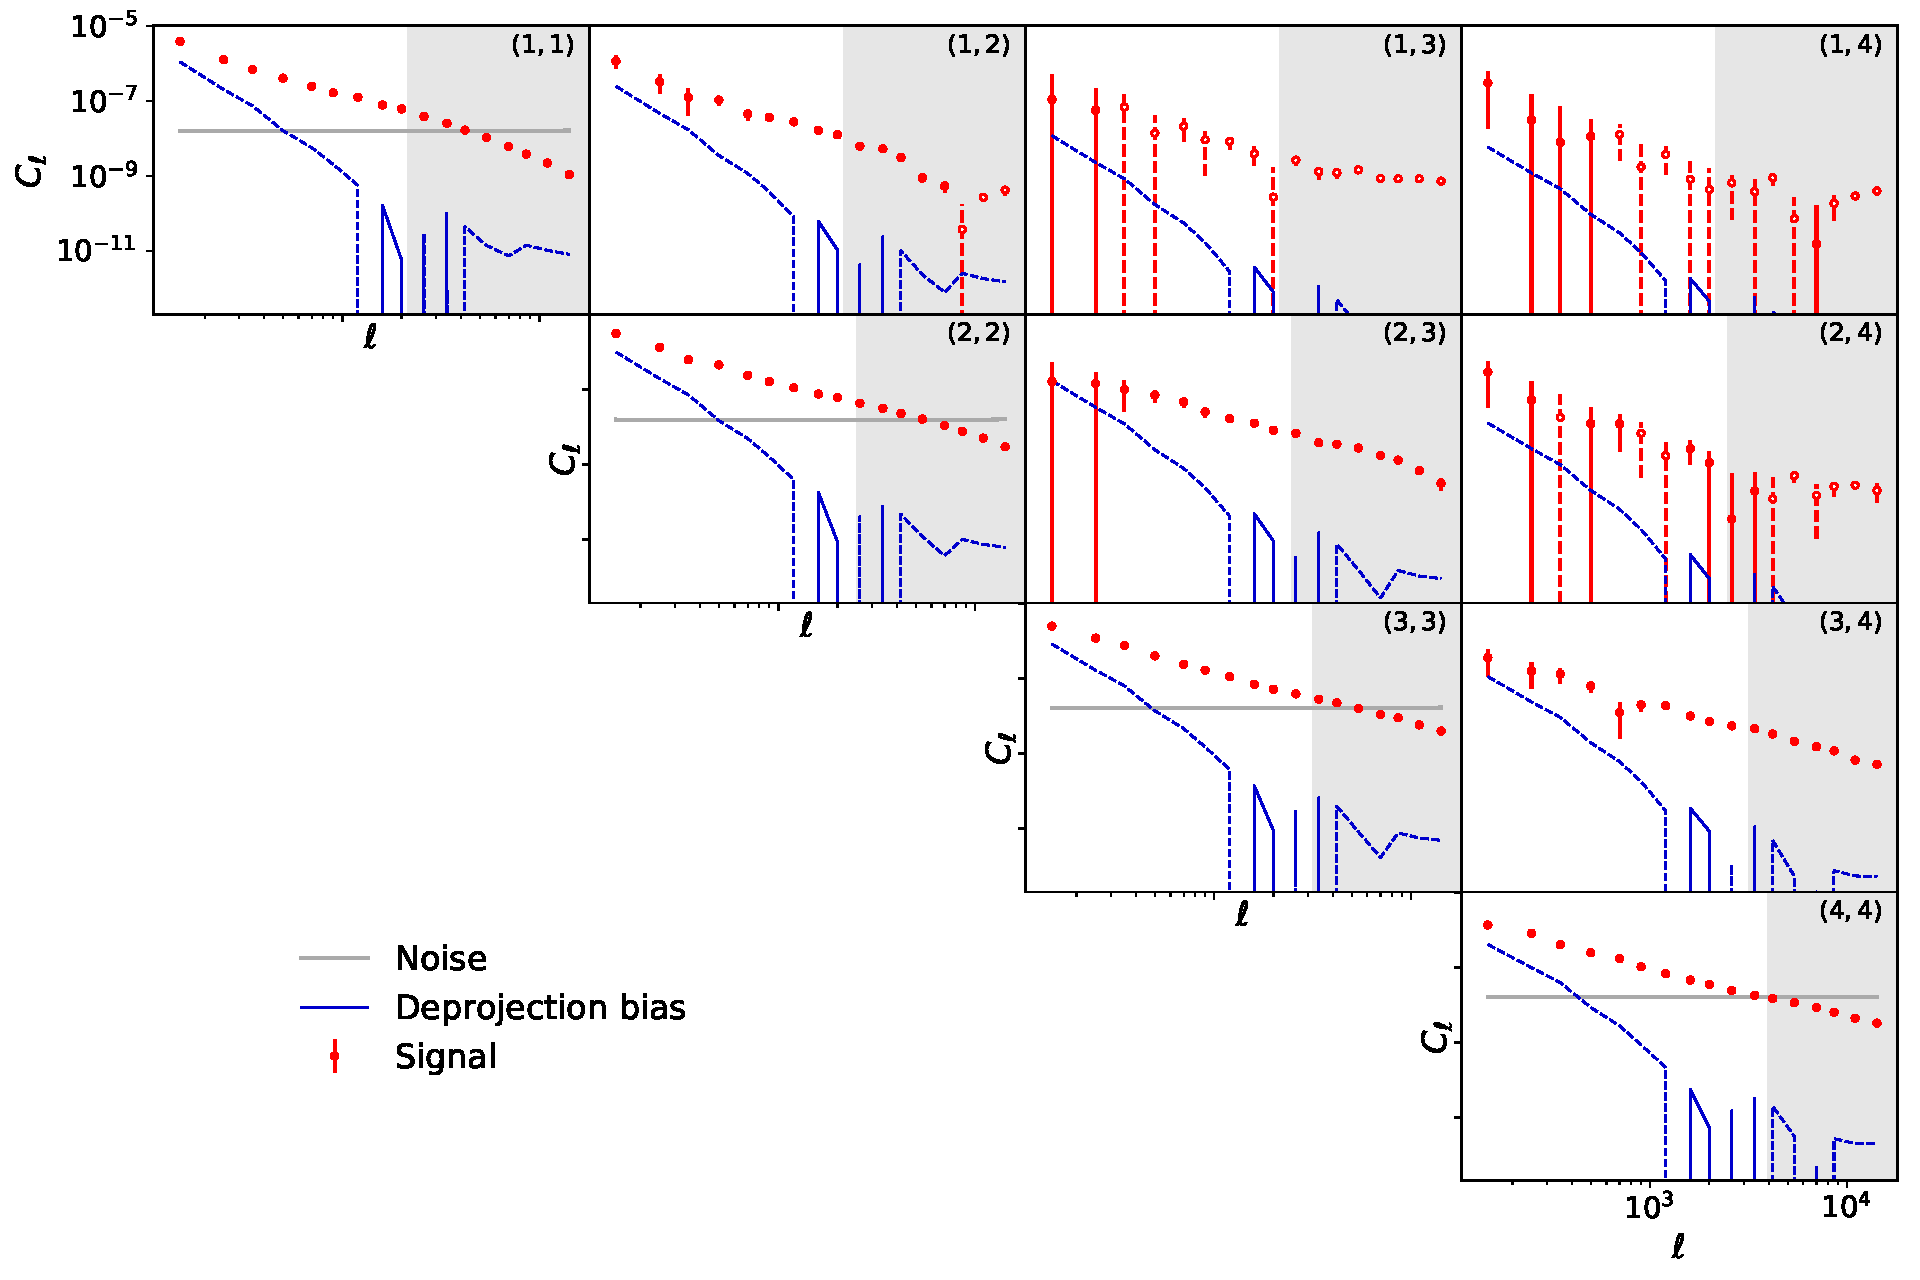
\includegraphics[width=0.99\textwidth]{figures/cls_summary.pdf}
        \caption{Summary plot showing all measured auto- and cross-power spectra. The red data points with error bars show the coadded power spectra (see Section \ref{sssec:results.spectra.fid}), with the hollow circles showing the absolute value of negative data. The Poisson noise contribution and deprojection biases subtracted from the raw power spectra are shown as grey and blue lines respectively, with the negative parts of the deprojection bias shown as dashed lines. The pair of numbers in the upper right corner of each panel corresponds to the indices of the bins being cross-correlated.}
        \label{fig:cls_summary}
      \end{figure}
      We compute all auto- and cross-power spectra between the four different redshift bins (listed in Table \ref{tab:bins_summary}) in each of the 6 HSC DR1 fields (listed in Table \ref{tab:field_summary}) as described in Section \ref{ssec:methods.cell}, including the deprojection of 48 different contaminant templates (9 observing condition maps in each of the 5 HSC filters, a dust map, a star density map and a depth map). In order to use these measurements to constrain model parameters, we first coadd them into a single set of spectra. We perform this coaddition simply as a weighted average, weighting the spectra in each field by their area:
      \begin{equation}
        {\bf C}_{\rm coadd}=\frac{\sum_f A_f\,{\bf C}_f}{\sum_f A_f}, \hspace{12pt}{\sf Cov}_{\rm coadd}=\frac{\sum_f A_f^2\,{\sf Cov}_f}{\left(\sum_f A_f\right)^2}
      \end{equation}
      where ${\bf C}$ is a vector containing all power spectra, ${\sf Cov}$ is its covariance matrix, and $f$ runs through the 6 DR1 fields with area $A_f$. This procedure should be close to inverse-variance weighting assuming that the power spectrum covariance has a similar structure in all fields. The coadded spectra should therefore be close to optimally weighted, with the added advantage that the coaddition does not introduce additional scale dependence due to mode-coupling in the covariance matrix.
      
      The resulting power spectrum measurements are shown in Figure \ref{fig:cls_summary} as red circles with error bars. In all cases we have subtracted the shot noise bias as described in Section \ref{ssec:methods.cell}, which is also shown as a grey solid line in the auto-correlations. As described in Section \ref{ssec:methods.cell}, after deprojecting a set of contaminant templates, the power spectra estimated from the projected maps must be corrected for a bias caused by the loss of modes due to deprojection. This bias is also shown as a blue solid line in Figure \ref{fig:cls_summary}, where the dashed parts show the absolute value of the bias when it is negative. This bias is always at least a factor $\sim5$ smaller than the measured power spectra, and is most relevant on large scales. The semi-transparent grey bands in the figure cover the range of scales excluded from our analysis (described in Section \ref{ssec:methods.constr}). Unless otherwise stated, in what follows all our results will not include any of these data.
      
      The rest of this sub-section describes the different tests we have carried out to quantify the robustness of these measurements.

    \subsubsection{Consistency across fields}\label{sssec:results.spectra.consistent}
      The fact that the HSC DR1 sample is distributed across 6 different disconnected fields allows us to carry out consistency tests of the measurements in individual fields. For example, it is reasonable to expect that, if a given undetected systematic is biasing our measurements significantly, its impact would vary across different fields, and would therefore lead to inconsitent power spectrum measurements between them. We carry out two basic consistency tests, involving the number density of objects in each field (i.e. the one-point function) and the measured power spectra.
      
      \paragraph{Number densities.} The number density of galaxies estimated in a given field is simply given by the ratio of the number of galaxies and the area of the field:
      \begin{equation}
        \hat{\bar{n}}=\frac{\sum_p N_p}{\sum_p \Omega_p}= \bar{n} \frac{\int \mathrm{d}\nv^2\,W(\nv)\left[1+\delta_g(\nv)\right]}{\int \mathrm{d}\nv^2\,W(\nv)},
      \end{equation}
      where $p$ runs over all pixels in the map, and $N_p$ and $\Omega_p$ are the number of objects and area of pixel $p$. In the second equality we have taken the continuum limit, $\bar{n}$ is the true number density, $\delta_g$ is the galaxy overdensity and $W$ is the field's mask. Using the statistics of $\delta_g$ it is straightforward to calculate the variance of the estimated $\hat{\bar n}$:
      \begin{equation}
       {\rm Var}(\hat{\bar n})=\int \frac{\mathrm{d}{\bf l}^2}{(2\pi)^2}\left|\frac{W_{\bf l}}{\int d\nv^2\,W(\nv)}\right|^2\,C_\ell.
      \end{equation}
      Here ${\bf l}$ is a 2D Fourier-space wave vector, $W_{\bf l}$ is the Fourier transform of the mask and $C_\ell$ is the power spectrum of $\delta_g$\footnote{We verified the validity of this calculation by replacing $C_\ell$ by its shot-noise contribution and recovering the Poisson limit (${\rm Var}_{\rm Poisson}(\hat{\bar n})=\bar{n}/A$, where $A$ is the footprint area). We find that the error on $\hat{\bar n}$ is dominated by cosmic variance (as opposed to shot noise) by more than a factor of $\sim5$ in all cases.}. Following this procedure we estimate the number density in each field and redshift bin as well as its uncertainty (where we use the mask described in Section \ref{ssec:methods.mask} and the best-fit theory power spectra to compute the latter). The results are shown in Figure \ref{fig:ndens_consistency}. In all cases we find no significant deviations in the number density found in each field with respect to the mean, with only one estimate out of the 24 (GAMA15H in bin 2) deviating by more than 2 $\sigma$. We therefore conclude that there is no evidence of inconsistency between fields on the basis of their number densities.
      \begin{figure}
        \centering
        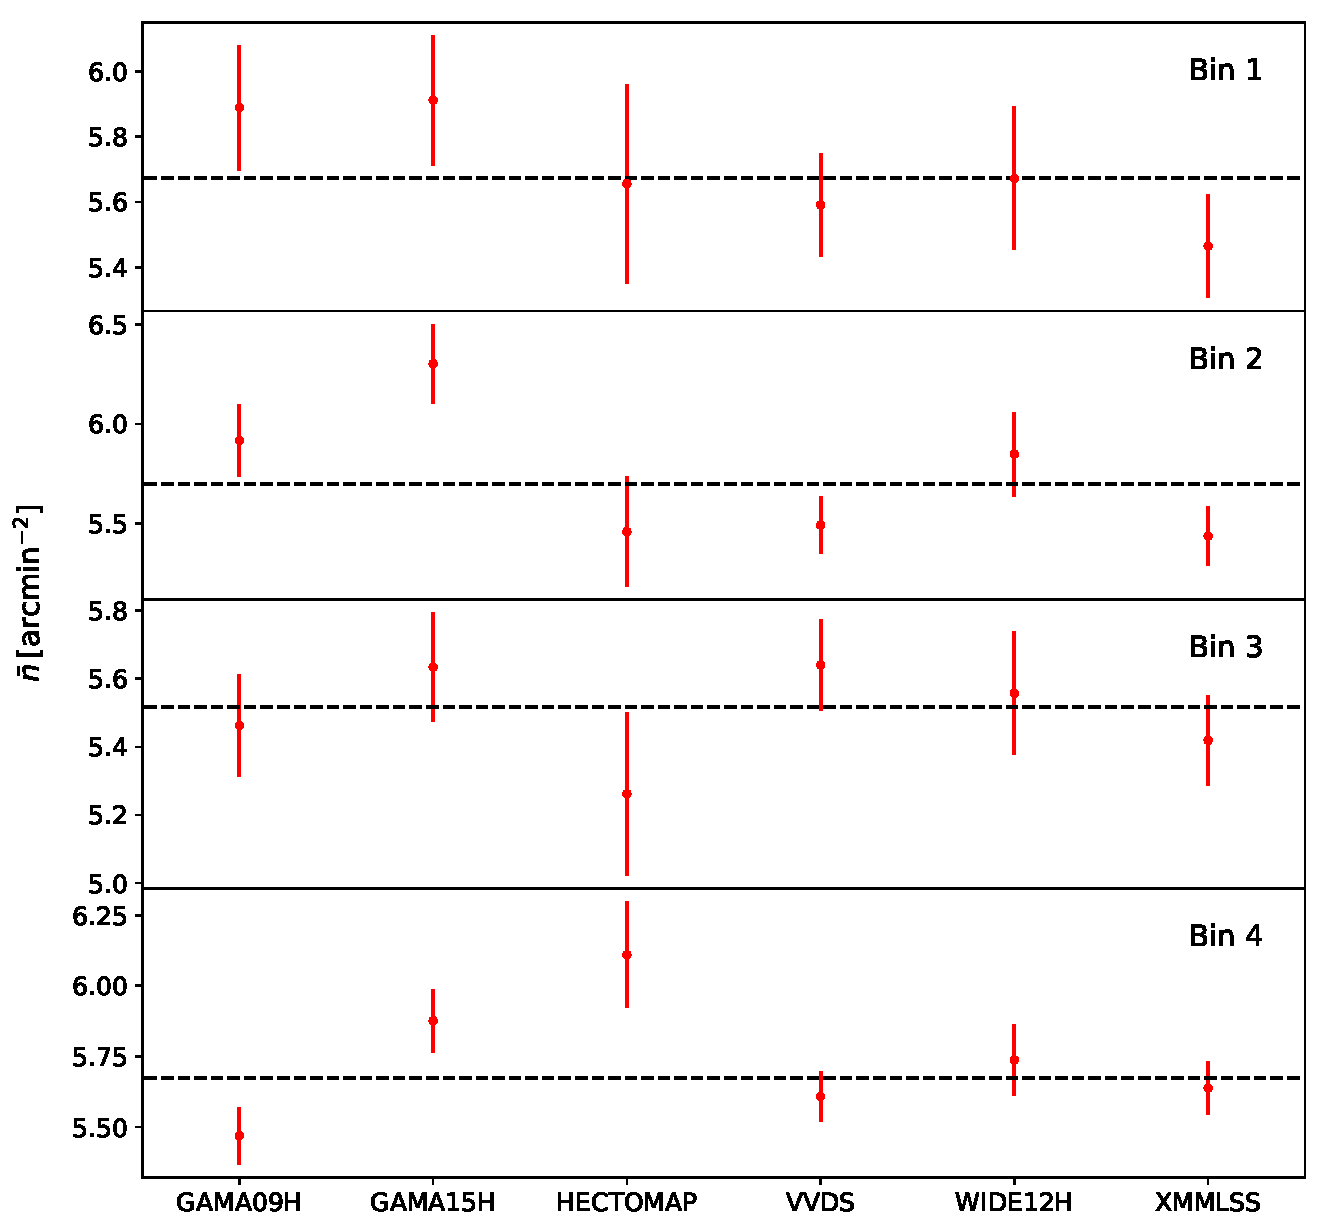
\includegraphics[width=0.7\textwidth]{figures/ndens_consistency.pdf}
        \caption{Source number densities estimated in the 6 different fields ($x$-axis) and in the 4 different redshift bins (in each panel, from top to bottom). We find no evidence of inconsistency between the number of sources found in each field.}
        \label{fig:ndens_consistency}
      \end{figure}

      \paragraph{Power spectra.} Figure \ref{fig:cls_consistency} shows the difference between the power spectra estimated in each field and the coadded power spectra normalized by the power spectrum errors for all auto- and cross-correlations. We observe a reasonable scatter with respect to the coadded spectra of up to $\sim3\sigma$, which does not immediately indicate any evidence for inconsistency between fields. As a more quantitative check for inconsistencies we carry out a $\chi^2$ analysis of this scatter. Let  $\Delta {\bf C}_f={\bf C}_f-{\bf C}_{\rm coadd}$ be the difference between the power spectra measured in field $f$ and the coadded ones. Using the notation of Section \ref{sssec:results.spectra.fid}, the covariance of $\Delta {\bf C}_f$ is given by:
      \begin{equation}
        {\sf Cov}_{\Delta_f}=\left(1-2\frac{A_f}{\sum_{f'}A_{f'}}\right){\sf Cov}_f+{\sf Cov}_{\rm coadd}.
      \end{equation}
      We can therefore quantify the significance of the power spectrum differences by computing the $\chi^2$:
      \begin{equation}
        \chi^2\equiv\Delta{\bf C}_f^T\cdot{\sf Cov}_{\Delta_f}^{-1}\cdot\Delta{\bf C}_f,
      \end{equation}
      and its probability to exceed (PTE) under the assumption that $\chi^2$ follows a ``chi-squared'' distribution with a number of degrees of freedom given by the size of $\Delta{\bf C}_f$. Doing so for all the individual auto- and cross-correlations, as well as for the combined data vector containing all of them simultaneously, we find no quantitative evidence of inconsistency between fields. All PTEs are larger than 8\%, with the vast majority of them lying above 30\%. We conclude that there is no evidence for systematics from the power spectrum measurements in different fields, and therefore it is safe to coadd them and use the coadded spectra to obtain model constraints.
      \begin{figure}
        \centering
        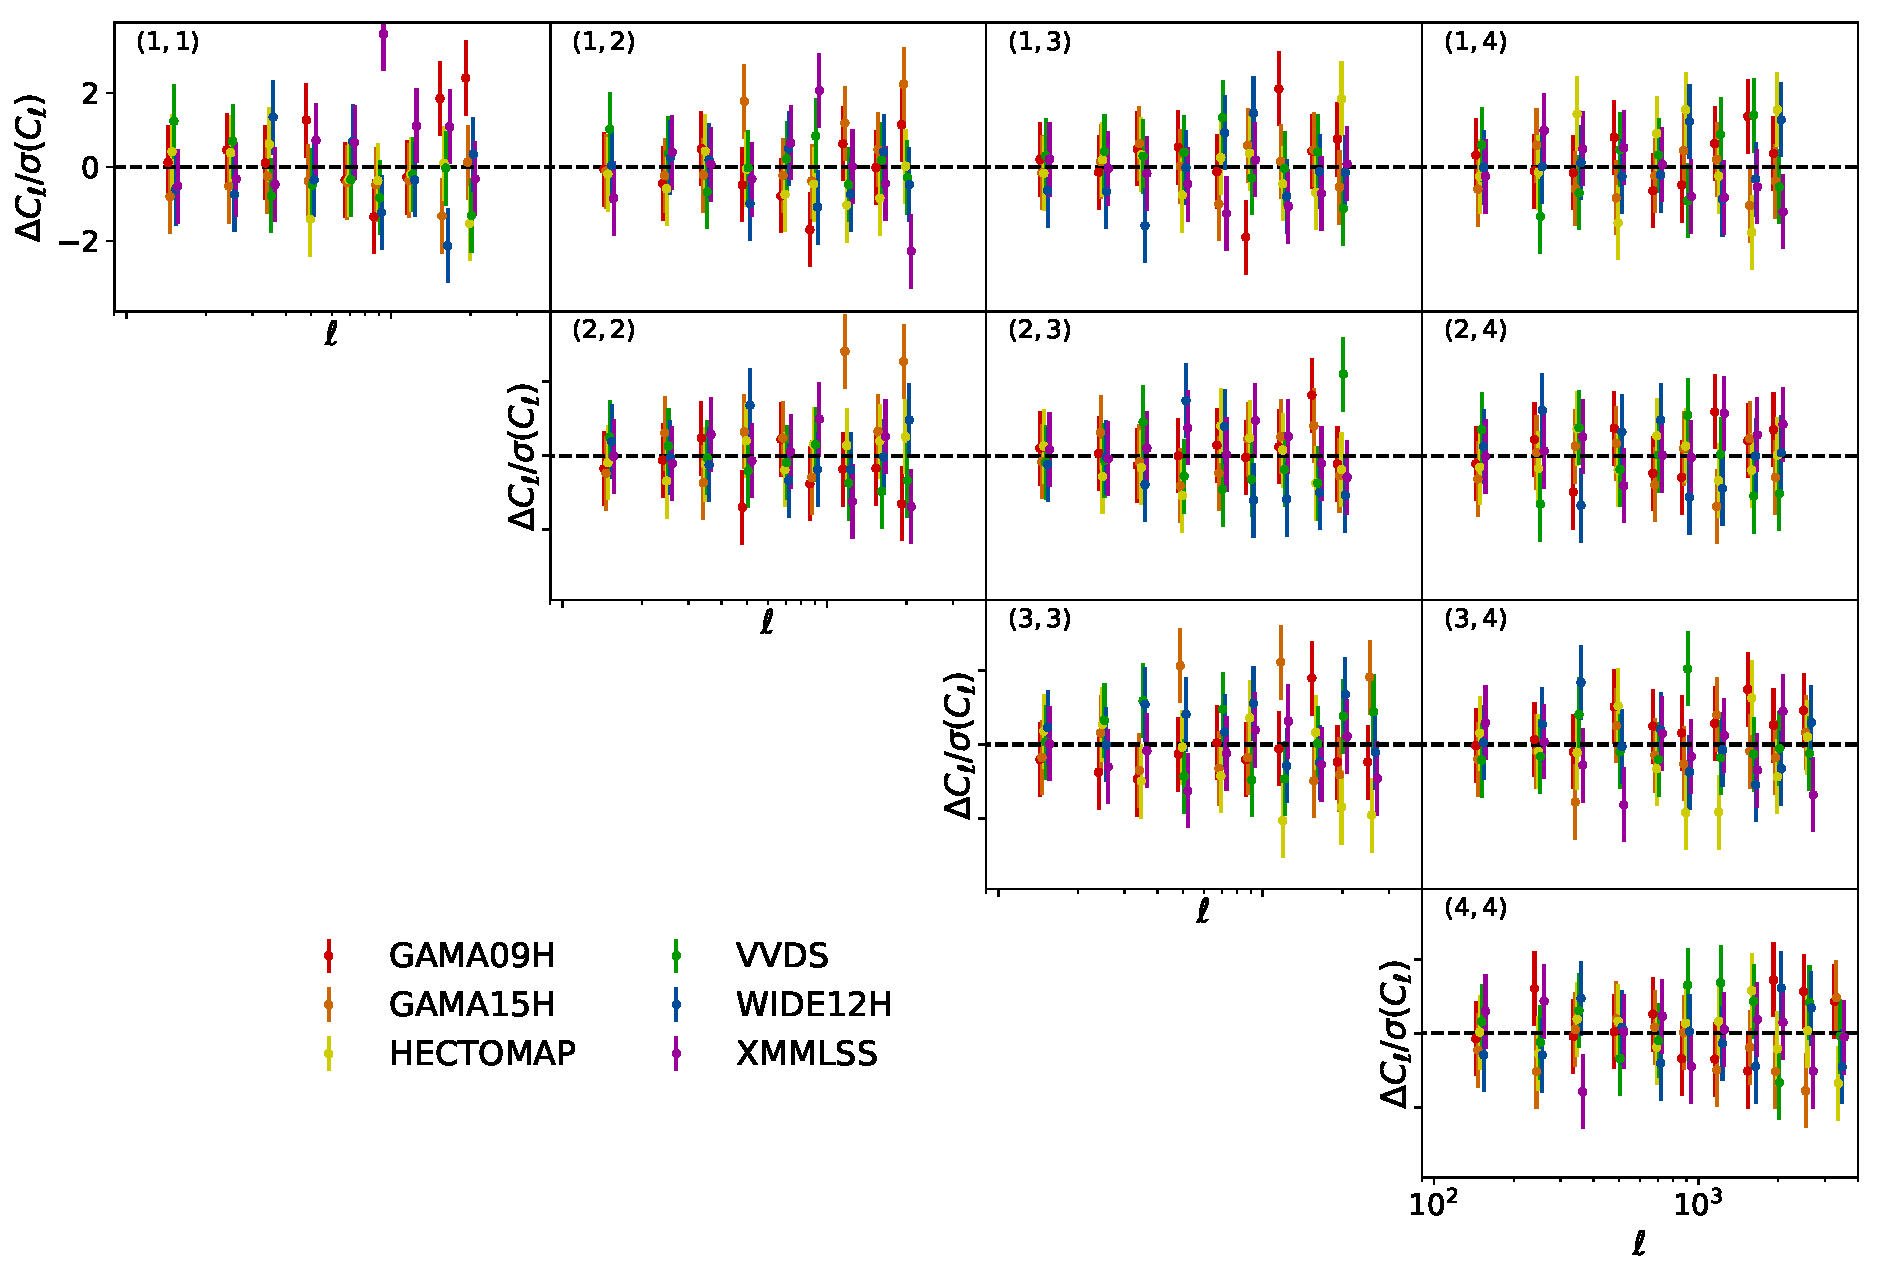
\includegraphics[width=0.99\textwidth]{figures/cls_consistency.pdf}
        \caption{Difference between the power spectra measured in each field and the mean coadded spectra normalized by the 1$\sigma$ errors. The pair of numbers in the upper right corner of each panel corresponds to the indices of the bins being cross-correlated. We find no inconsistency between the different measurements.}
        \label{fig:cls_consistency}
      \end{figure}
      
    \subsubsection{Robustness to contaminants} \label{sssec:results.spectra.syst}
      \begin{figure}
        \centering
        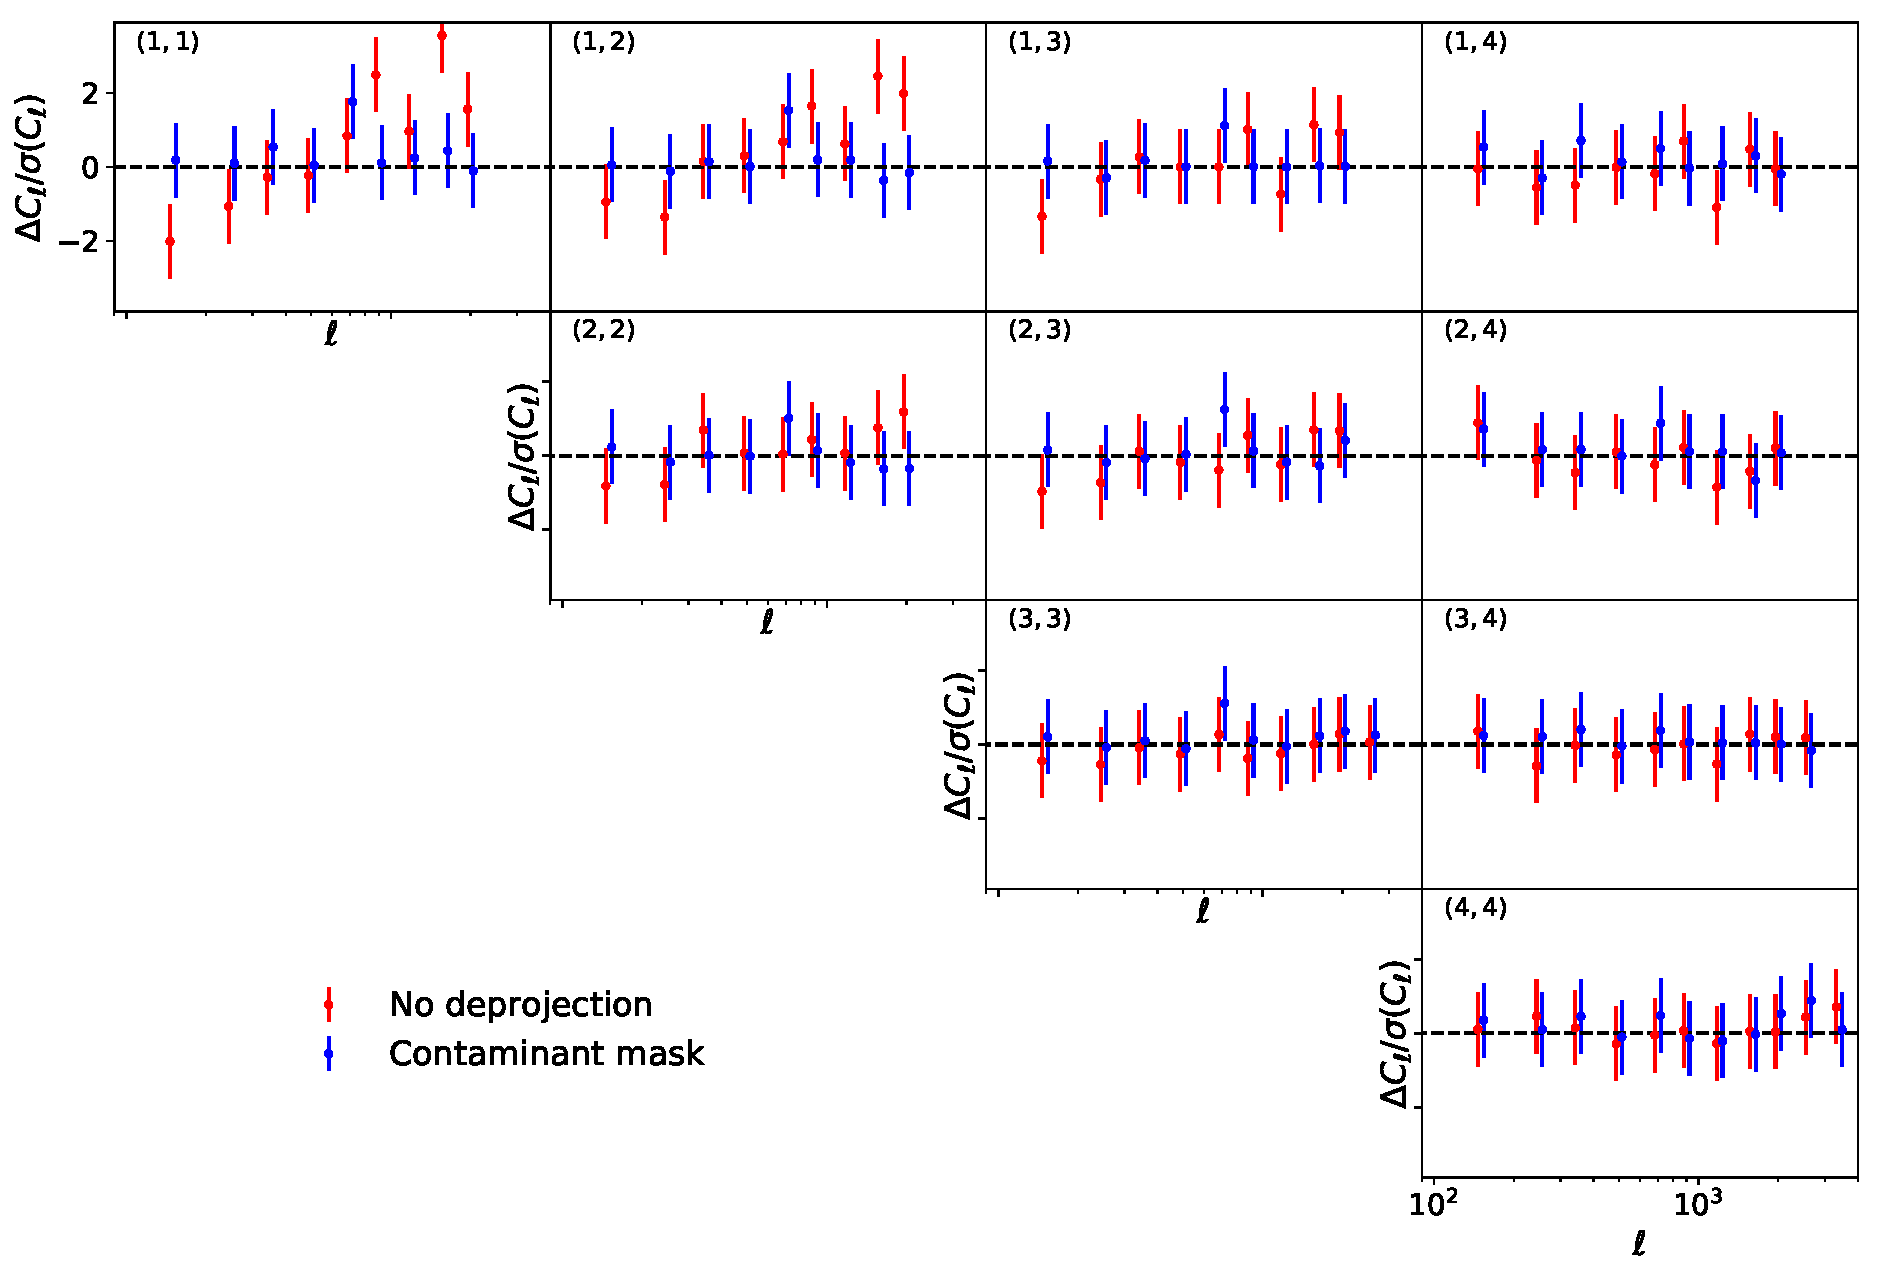
\includegraphics[width=0.99\textwidth]{figures/cls_systematics.pdf}
        \caption{Difference with respect to our fiducial power spectra of alternative estimates of the power spectra normalized by their $1\sigma$ errors. The red points show the spectra estimated without contaminant deprojection. The blue points show spectra estimated using a conservative sky mask that removes highly contaminated regions (see Section \ref{sssec:results.spectra.syst} for details). The yellow points show the spectra calculated using the Arcturus bright star mask.}
        \label{fig:cls_systematics}
      \end{figure}
      As described in Section \ref{ssec:methods.cell}, our main strategy to address possible contamination of the measured power by systematics causing artificial density fluctuations is to project out the systematics templates discussed above from the data at the map level. This procedure can also be understood as building a linear model for the contamination (see Eq. \ref{eq:deproj1}), finding the best-fit linear coefficients for each contaminant and substracting the corresponding contribution from the observed map. Finally, the estimated power spectra must be corrected for the loss of modes incurred (blue line in Figure \ref{fig:cls_summary}). This method is therefore able to account for any systematic contamination that is well described as a linear contribution. Since the impact of any contaminant can always be Taylor-expanded, this treatment is appropriate as long as the level of contamination is sufficiently small. In order to verify this, we have carried out two different tests.
      
      First, we have compared our fiducial power spectra, computed using contaminant deprojection, with power spectra computed without accounting for any type of contamination (i.e. estimated directly from the observed galaxy overdensity maps). This test allows us to test the worst-case scenario where any source of contamination is completely ignored. The result, shown as the differences between both power spectra normalized by their 1$\sigma$ uncertainty, is shown in red in Figure \ref{fig:cls_systematics}. In most cases we observe very small differences (smaller than $1\sigma$) between both spectra. However, we see that some of the spectra involving the first redshift bin are slightly more sensitive to deprojection, exhibiting differences of up to 3$\sigma$ in the range of scales used in our analysis. This suggests that, although the level of contamination in the raw galaxy overdensity maps is small, it is necessary to address it.
      \begin{figure}
        \centering
        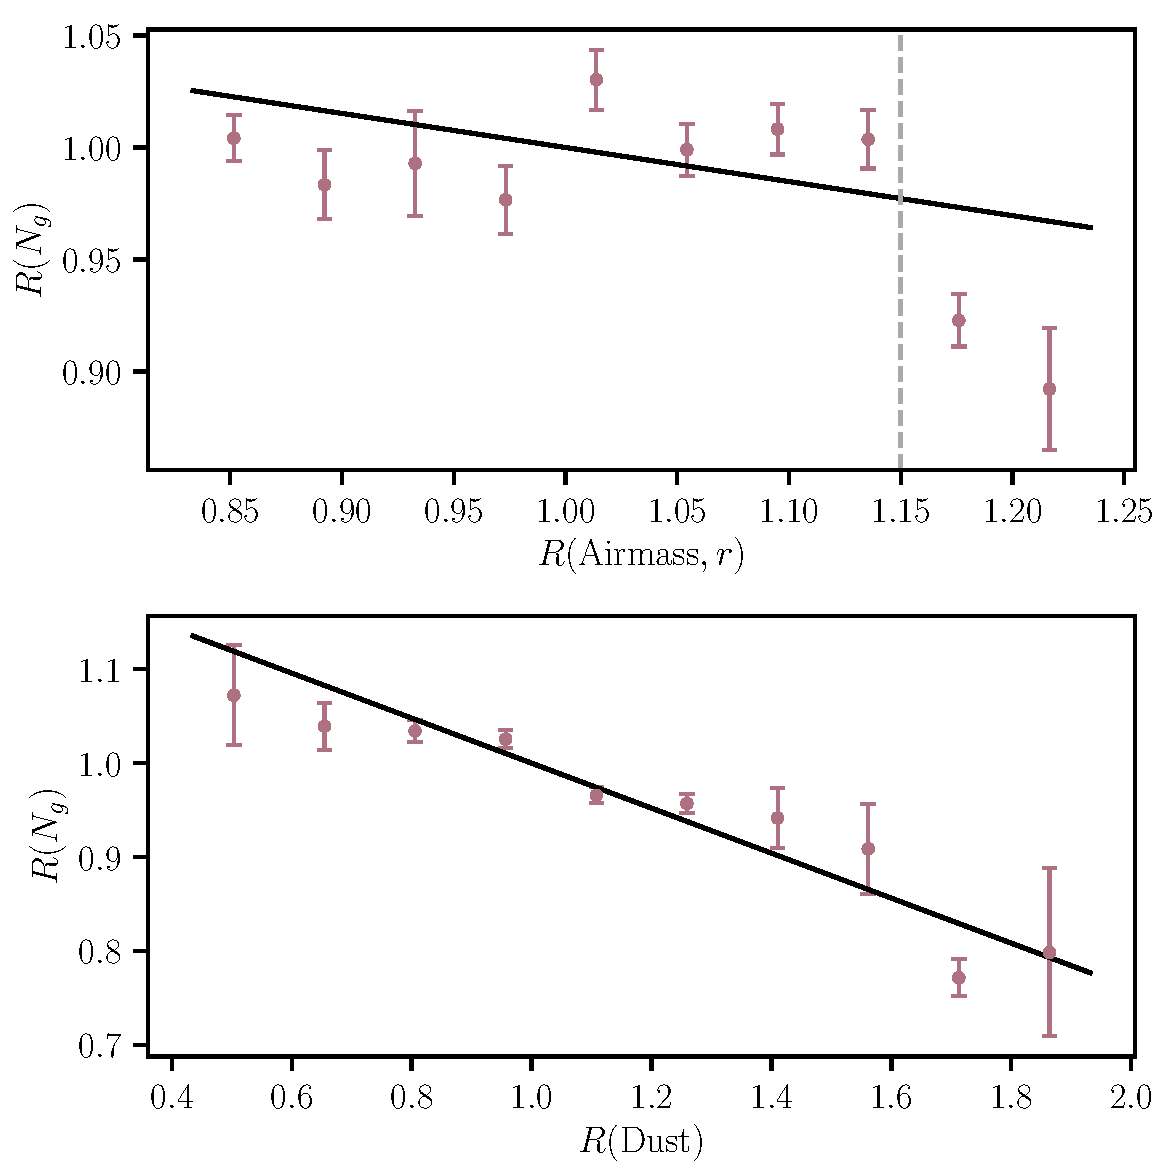
\includegraphics[width=0.49\textwidth]{figures/ndens_syst.pdf}
        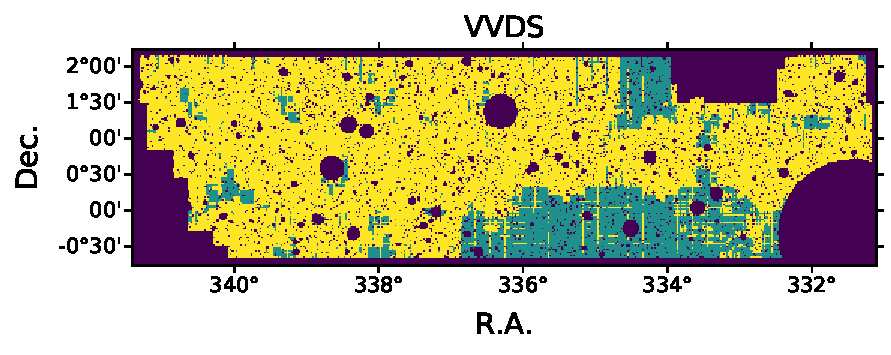
\includegraphics[width=0.49\textwidth]{figures/systmask.pdf}
        \caption{{\sl Left panels:} relation between the galaxy density fluctuation ($y$ axis) and the fluctuation in different systematics ($x$-axis). In all cases $R(x)\equiv \sfrac{x}{\bar{x}}$. Results are shown for $r$-band airmass (top) and dust absorption (bottom) for the third redshift bin in the VVDS field. The data are shown in red, while the solid black line shows the best-fit linear relation between both quantities. In cases where a linear relation is not appropriate (as shown here for $r$-band airmass), we mask all regions where the associated contaminant is above/below a given threshold (shown as a vertical dashed line here). {\sl Right panels:} the top panel shows our fiducial ``Sirius'' mask, with the additionally masked regions associated with high levels of contamination shown in turquoise. The bottom panel shows the alternative ``Arcturus'' bright-star mask.}
        \label{fig:ndens_syst}
      \end{figure}
      
      Second, in order to explore the breakdown of the linear model used in deprojection, we have made a direct study of the relation between galaxy overdensity and the different systematics as follows: for each field and redshift bin we produce a map of the relative galaxy density $R(N_g)\equiv N_g(\nv)/\bar{N}_g$, where $N_g(\nv)$ is the number of galaxies in the pixel with coordinates $\nv$, and $\bar{N}_g$ is the mean number of galaxies per pixel across the map. Then, for each of the 48 systematic templates $S$, we create a similar map $R(S)\equiv S(\nv)/\bar{S}$. We then use both maps to calculate the mean value of $R(N_g)$ in bins of $R(S)$, estimating the error on this mean via bootstrap. Finally, we produce plots of this relation for all fields, bins and systematic maps, finding results such as those displayed in the left panels of Figure \ref{fig:ndens_syst}, which show this relation for bin 3 of the VVDS field for the dust absorption and $r$-band airmass templates (bottom and top panels respectively). In most cases we find that the relation between galaxy density and systematic fluctuation is either flat or well approximated by a linear relation, as is the case for dust absorption in the figure. In a few cases, however, we find that a linear relation is only appropriate in parts of the range of contaminant values, and that the observed galaxy overdensity grows or decreases much faster for large or small values of $R(S)$. In these cases, fitting a linear relation over the whole range of $S$ will lead to some level of contaminant residuals that could induce a significant bias on the estimated power spectra. To verify whether this is the case, we list all cases where we find that a linear relation is not appropriate, determine the value of $R(S)$ beyond which we observe a significant increase/decrease in $R(N_g)$ (shown as a vertical dashed line in the top left panel of Figure \ref{fig:ndens_syst} for $r$-band airmass), and mask out the corresponding regions of the map. The masked regions correspond to $\sim20\%$ of the available footprint on average, and are shown in the top right panel of Figure \ref{fig:ndens_syst} in turquoise for the VVDS field. The blue datapoints in Figure \ref{fig:cls_systematics} show the difference with respect to our fiducial power spectra of the power spectra estimated using these more restrictive masks, normalized by their $1\sigma$ errors. In the vast majority of cases we see only $<1\sigma$ differences between both spectra. Since small differences are to be expected when masking a significant fraction of the observed footprint, we conclude that there is no evidence of contamination in our fiducial power spectra beyond that accounted for by the template deprojection procedure.

      One final possible source of systematic bias is the effect of bright sources, which cause a depletion in the number of observed galaxies around them as described in e.g. \cite{2018PASJ...70S...7C}. To mitigate this effect we make use of the bright object mask provided with the HSC DR1 (the so-called ``Sirius'' mask) as described in Section \ref{ssec:methods.mask}. One possible problem associated with this mask is the fact that it removes regions around both bright stars as well as a small fraction of bright extra-Galactic objects. Since the latter will be correlated at some level with some of the sources used in our clustering analysis, it is important to check for a possible bias associated with masking them. To do so, and to test our fiducial power spectra against the exact procedure used to produce the bright object mask, we have repeated our measurements making use of the bright star mask published by \cite{2018PASJ...70S...7C} (the so-called ``Arcturus mask). The top-right and bottom-right panels of Figure \ref{fig:ndens_syst} show both masks for the VVDS field. We can see that, while the masked regions are mostly centered around the same sources, the prescriptions used to define the masking radii are different \todo{we could give some details of what the differences are here}. The yellow datapoints in Figure \ref{fig:cls_summary} show the difference with respect to our fiducial power spectra of the spectra computed using the Arcturus mask, normalized by their 1$\sigma$ errors. As before, we do not observe any statistically significant deviation between these spectra. We therefore conclude that bright sources do not impact our fiducial power spectra significantly. 
      
    \subsubsection{Shot noise subtraction} \label{sssec:results.spectra.shotnoise}
      \begin{figure}
        \centering
        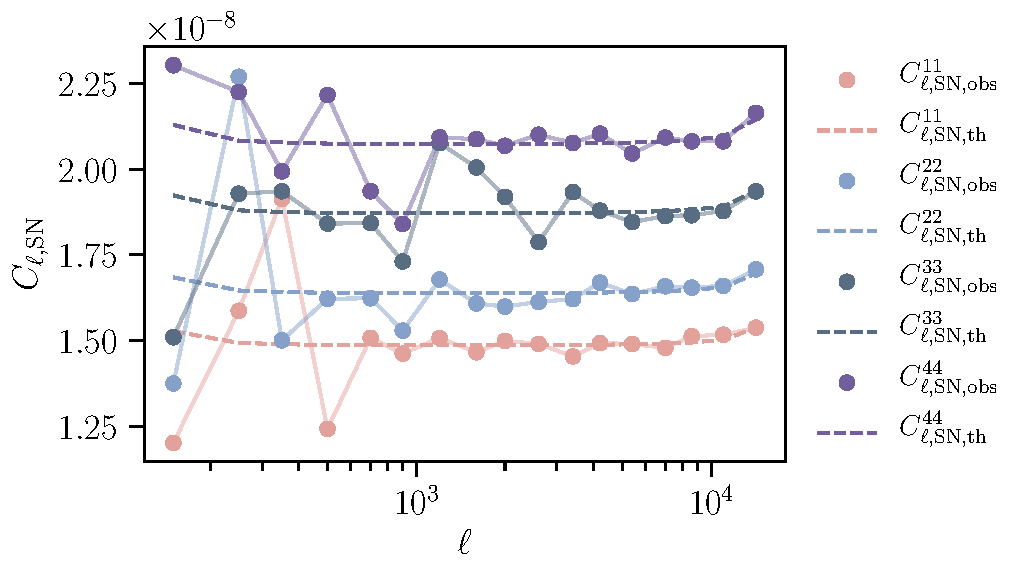
\includegraphics[width=0.6\textwidth]{figures/shotnoise_avg.pdf}
        \caption{Comparison between the shot noise power spectra estimated analytically using Eq. \ref{eq:nell} (transparent lines) and estimated from the difference-map power spectra (solid lines). Results are shown for the four different redshift bins. Our analytic estimate agrees well with this alternative method.}
        \label{fig:shotnoise_avg}
      \end{figure}
      As described in Section \ref{ssec:methods.cell}, we subtract the shot-noise contribution to the auto-correlation power spectra using an analytical estimate, given by Eq. \ref{eq:nell}. Since it has been argued \citep{2013PhRvD..88h3507B} that non-linearities may produce deviations from this simple relation, we verify the validity of our calculation as follows.
      
      We start by splitting the galaxy sample in each field into two random subsamples with the same number of objects.  We then construct overdensity maps for each of the galaxy subsamples, which we call $\delta_1$ and $\delta_2$.  Each of these subsamples can be thought of as an independent Poisson processes that samples the same underlying smooth overdensity field $\delta$. I.e. $\delta_i = \delta + n_i$, where $n_i$ is the shot-noise contribution in $\delta_i$. Therefore, we can estimate the shot-noise power spectrum from the power spectrum of the difference between the two split maps:
      \begin{align}
      \left\langle |\delta_1 - \delta_2|^2 \right\rangle & = \langle|n_1|^2\rangle + \langle|n_2|^2\rangle,
      \end{align}
      where we have assumed that $n_1$ and $n_2$ are uncorrelated (since our two sub-catalogs are disjoint). Since the number density in each of the subsamples is half of the full sample, we can recover an estimate of the latter's shot-noise spectrum by simply dividing the power spectrum of the difference map by $4$. Figure \ref{fig:shotnoise_avg} shows the comparison between the analytic estimate in Eq. \ref{eq:nell} (transparent lines) and the estimate from the difference map power spectra (solid lines) for the four different redshift bins \todo{what order?}. Within the statistical noise of the split-map estimate, both methods agree well, particularly at high $\ell$, validating our procedure to subtract the shot-noise contribution.
      
    
\subsection{Covariance matrix}\label{ssec:results.covariance}

We estimate the covariance matrix of all measured power spectra analytically as described in Sec.~\ref{sssec:methods.theory.covar} and the resulting correlation matrix is shown in Fig.~\ref{fig:covmat}. In Fig.~\ref{fig:covariance-contributions}, we split the auto-covariances for the four redshift bins into the Gaussian, non-Gaussian and SSC contributions. As can be seen, the Gaussian contribution is dominant on large scales while the non-Gaussian part becomes important at small scales and low redshift. The high redshift bins are mostly insensitive to non-Gaussian contributions to the covariance. Finally, the SSC is subdominant in all cases. This is mainly due to the number density correction in Eq.~\ref{eq:ps-resp}, which significantly suppresses any SSC contributions to the total covariance.

\begin{figure}
\begin{center}
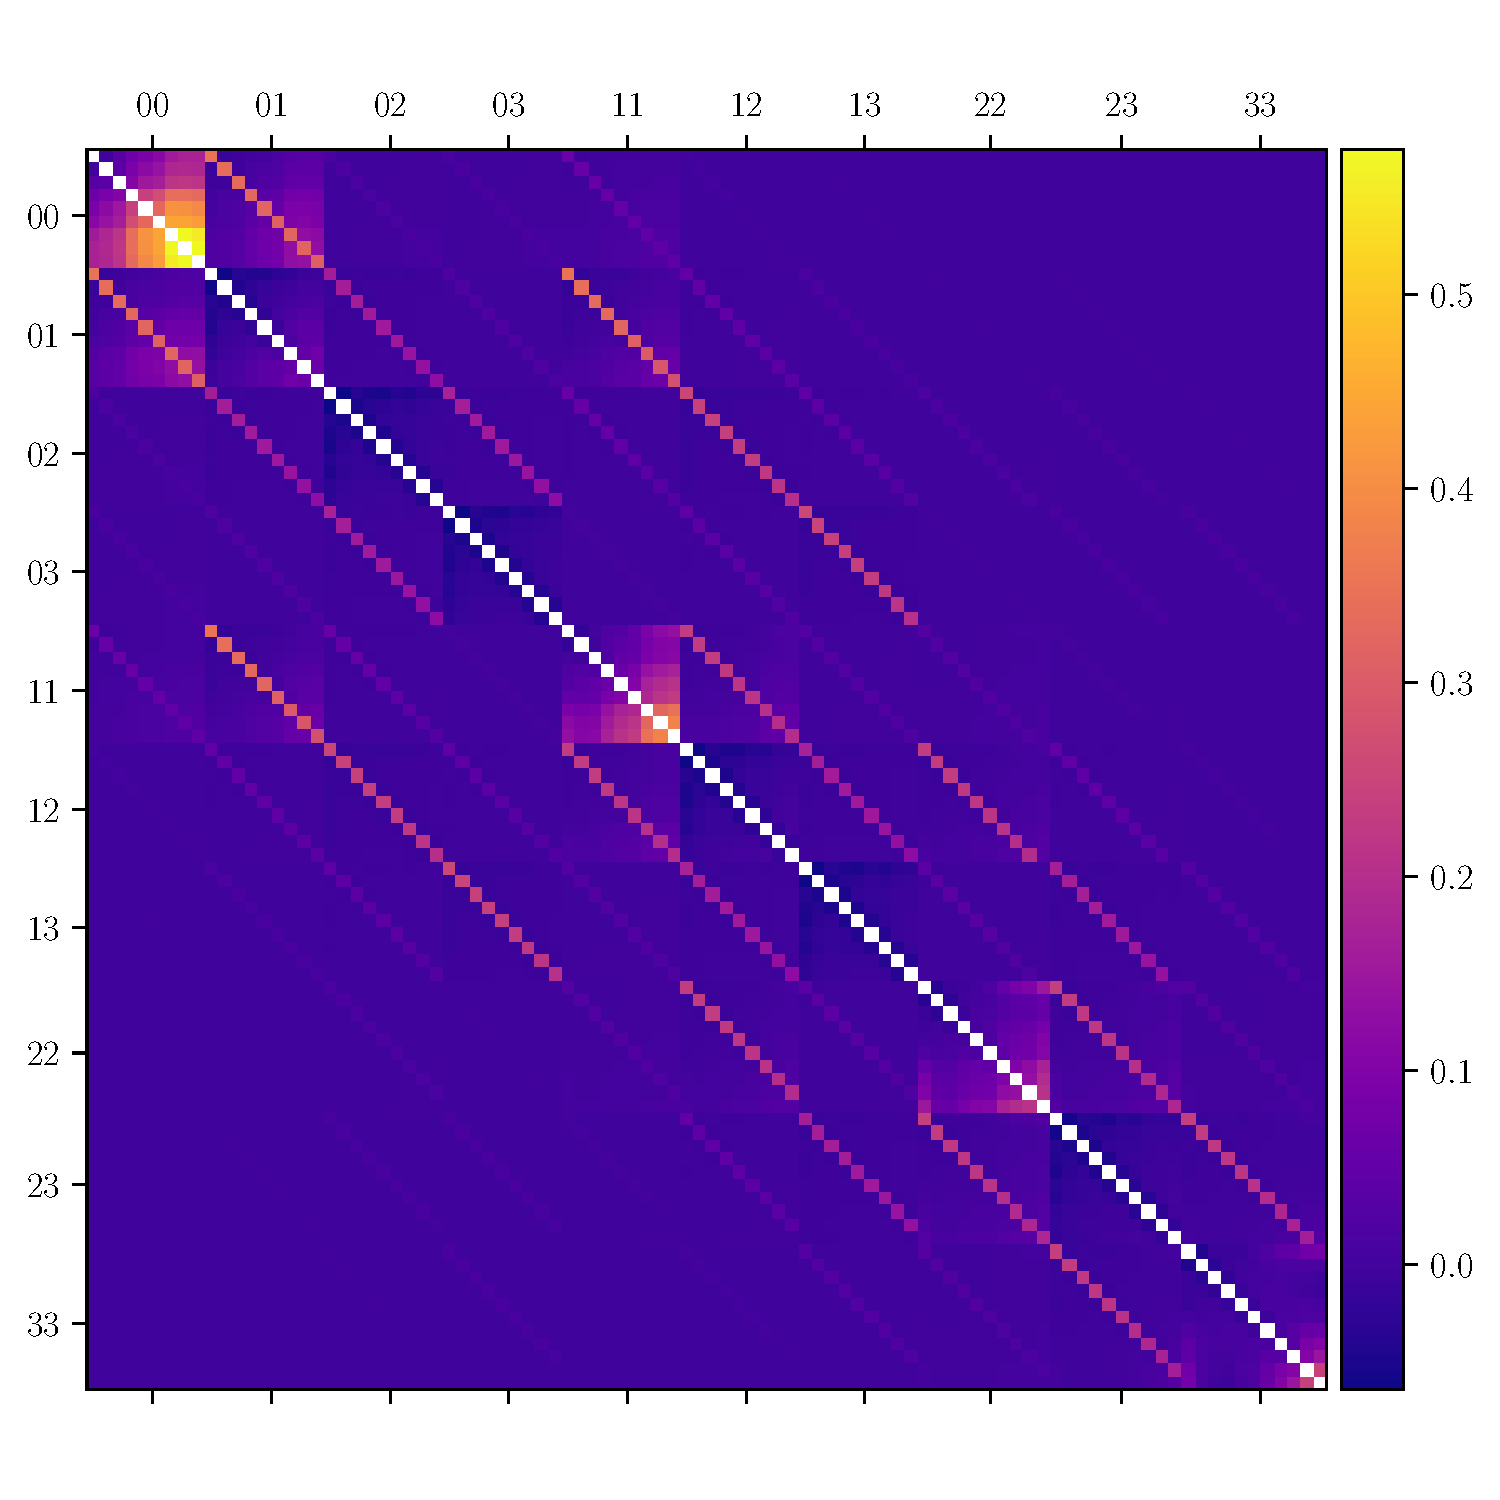
\includegraphics[width=0.5\textwidth]{figures/covmat_HSC_dg_hoddg_hodxdg_hoddg_hod_trisp=4h3h2h_SSC=LINBIAS-resp_l=ells_eff_all_wcross_clfit=HOD-zevol_culled=True_coadd=area_G+NG+SSC.pdf}
\caption{Correlation matrix for all auto- and cross power spectra considered in our analysis, estimated as described in Sec.~\ref{sssec:methods.theory.covar}.}
\label{fig:covmat}
\end{center}
\end{figure}

\begin{figure}
\begin{center}
\subfigure[$C_{\ell}^{00}$]{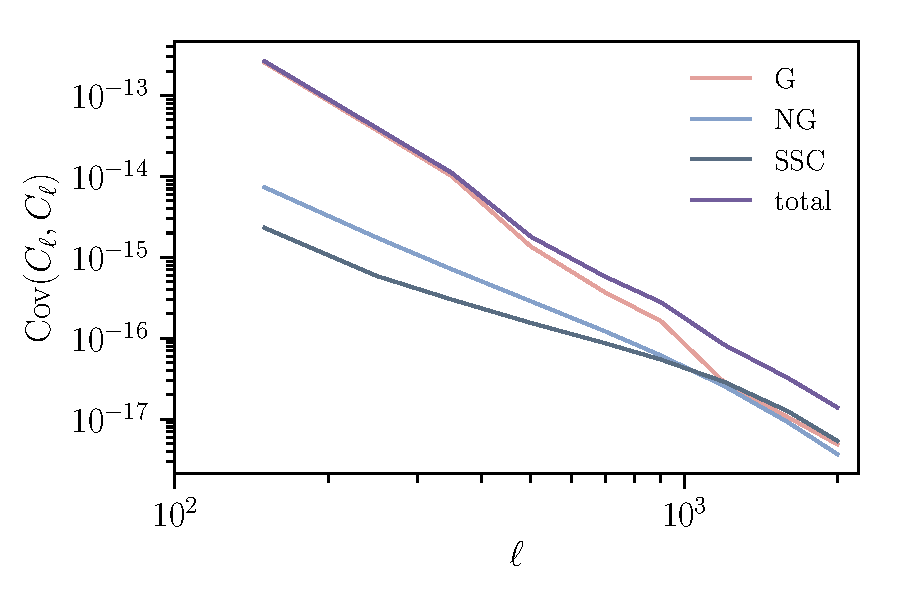
\includegraphics[width=0.49\textwidth]{figures/covmat_HSC_dg_hoddg_hodxdg_hoddg_hod_trisp=4h3h2h_SSC=LINBIAS-resp_l=ells_eff_all_wcross_clfit=HOD-zevol_culled=True_coadd=area_comparison=G+NG+SSC_bin=0.pdf}}
\subfigure[$C_{\ell}^{11}$]{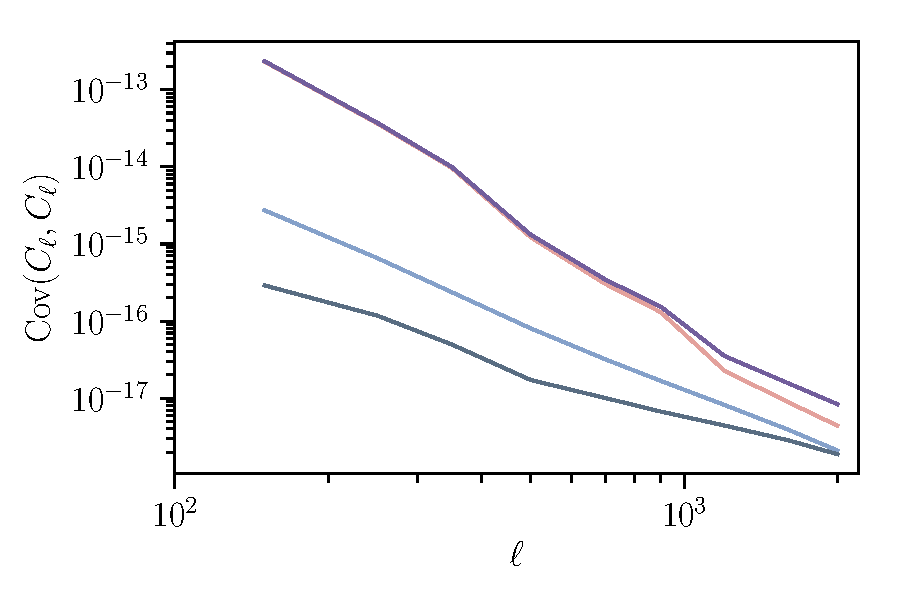
\includegraphics[width=0.49\textwidth]{figures/covmat_HSC_dg_hoddg_hodxdg_hoddg_hod_trisp=4h3h2h_SSC=LINBIAS-resp_l=ells_eff_all_wcross_clfit=HOD-zevol_culled=True_coadd=area_comparison=G+NG+SSC_bin=1.pdf}} \\
\subfigure[$C_{\ell}^{22}$]{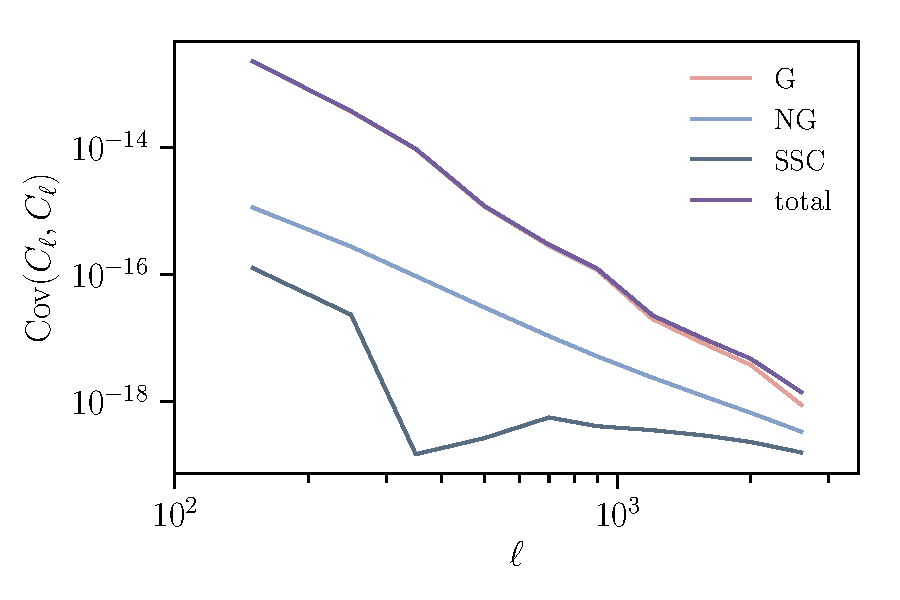
\includegraphics[width=0.49\textwidth]{figures/covmat_HSC_dg_hoddg_hodxdg_hoddg_hod_trisp=4h3h2h_SSC=LINBIAS-resp_l=ells_eff_all_wcross_clfit=HOD-zevol_culled=True_coadd=area_comparison=G+NG+SSC_bin=2.pdf}}
\subfigure[$C_{\ell}^{33}$]{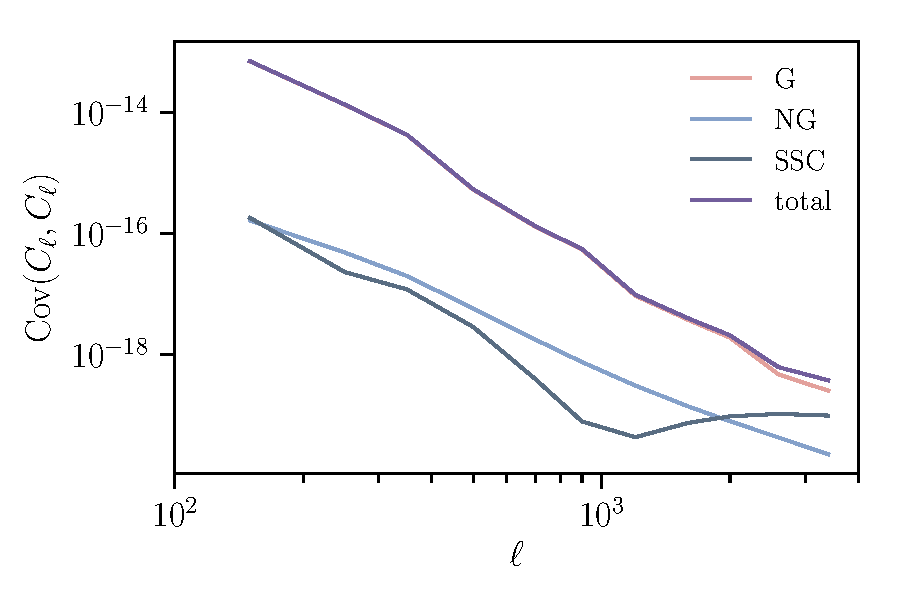
\includegraphics[width=0.49\textwidth]{figures/covmat_HSC_dg_hoddg_hodxdg_hoddg_hod_trisp=4h3h2h_SSC=LINBIAS-resp_l=ells_eff_all_wcross_clfit=HOD-zevol_culled=True_coadd=area_comparison=G+NG+SSC_bin=3.pdf}} 
\caption{Comparison of the different contributions to the covariance matrix for the four auto-power spectra considered in our analysis.} 
\label{fig:covariance-contributions}
\end{center}
\end{figure}

\subsection{Constraints on HOD parameters}\label{ssec:results.hod-constraints}

\subsubsection{Fiducial constraints}\label{sssec:results.hod-constraints.fiducial}

Both the auto- and cross power spectra shown in Fig.~\ref{fig:cls_summary} carry information on astrophysical, systematics and cosmological parameters. We especially expect the cross correlations to help constrain photo-$z$ systematics parameters, as they probe the relative clustering strength in different redshift bins and thus help break degeneracies between the clustering amplitude and shifts in the means of the bins. In this work, we therefore compute fiducial constraints from a joint fit to both auto- and cross power spectra.

Fig.~\ref{fig:constraints-fid-hod} shows the constraints on the HOD parameters $M_{\mathrm{min}}, \allowbreak \, M_{\mathrm{min}, p}, \allowbreak \, M_{1}, \allowbreak \, M_{1, p}$ for our fiducial model described in Sec.~\ref{ssec:methods.constr}. The constraints on all fitted parameters are shown in Fig.~\ref{fig:constraints-fid-full} and the corresponding best-fit values and means are shown alongside their $68 \%$ confidence limits in Tab.~\ref{tab:params}. As can be seen from Figures \ref{fig:constraints-fid-hod} and \ref{fig:constraints-fid-full}, the data allow us to constrain $M_{\mathrm{min}}(z)$ and $M_{1}(z)$ whereas $M_{0}(z)$ is unconstrained\footnote{In the following, we therefore only show constraints on the HOD parameters $M_{\mathrm{min}}, \, M_{\mathrm{min}, p}, \, M_{1}, \, M_{1, p}$.}. Fig.~\ref{fig:cls-best-fit} shows the theoretical predictions derived from maximum likelihood parameters together with our the measured power spectra. The corresponding minimum $\chi^{2}$ is $\chi^{2} = 86.2$. Computing the degrees of freedom as $\nu = N_{\mathrm{data}} - N_{\mathrm{param}} = 94 - 14 = 80$, we obtain $\chi^{2}_{\mathrm{red}} = \sfrac{\chi^{2}}{\nu} = 1.08$ ($p$-value $= 0.30$), which shows that the data are consistent with the best-fit theoretical model\footnote{We note that this estimate of the degrees of freedom is only valid for linear models and independent basis functions (see e.g. \cite{Andrae:2010}). However, we will use it throughout this work, as it allows us to obtain a rough estimate of the goodness of fit of the different models considered in our analysis.}.

In Fig.~\ref{fig:hod-params-z-dep} we show the redshift dependence of the minimal mass to host a central galaxy $M_{\mathrm{min}}(z)$ and the mass scale for satellites $M_{1}(z)$ obtained in our analysis. To illustrate the uncertainty on this relation, we also show a sample of curves derived from 1000 random realizations from the MCMCs. As can be seen, we find that, within or uncertainties, the data prefer both a constant $M_{\mathrm{min}}$ and $M_{1}$. This is somewhat counterintuitive, as we would naively expect at least the minimal mass to host a central galaxy to increase with redshift since galaxies will only form in the most massive halos at early times. We will discuss these findings in detail in Sec.~\ref{sssec:results.hod-constraints.constraints-interpretation}. Finally we see from Tab.~\ref{tab:constraints_robustness} that the minimal mass to host a satellite galaxy, $M_{0}(z)$, obtained in our analysis is quite low. This is a feature of our HOD model enforcing that no halo can host satellites if it does not contain a central galaxy, regardless of $M_{0}(z)$ (see Eq.~\ref{eq:ng_hod}). Therefore we find that the constraints on $M_{0}(z)$ are unbounded at low masses, i.e. the data constrain the maximal $M_{0}(z)$ to be of the order of $M_{\mathrm{min}}(z)$, but our HOD model does not allow us to distinguish between masses smaller than $M_{\mathrm{min}}(z)$.
  
\begin{figure}
\begin{center}
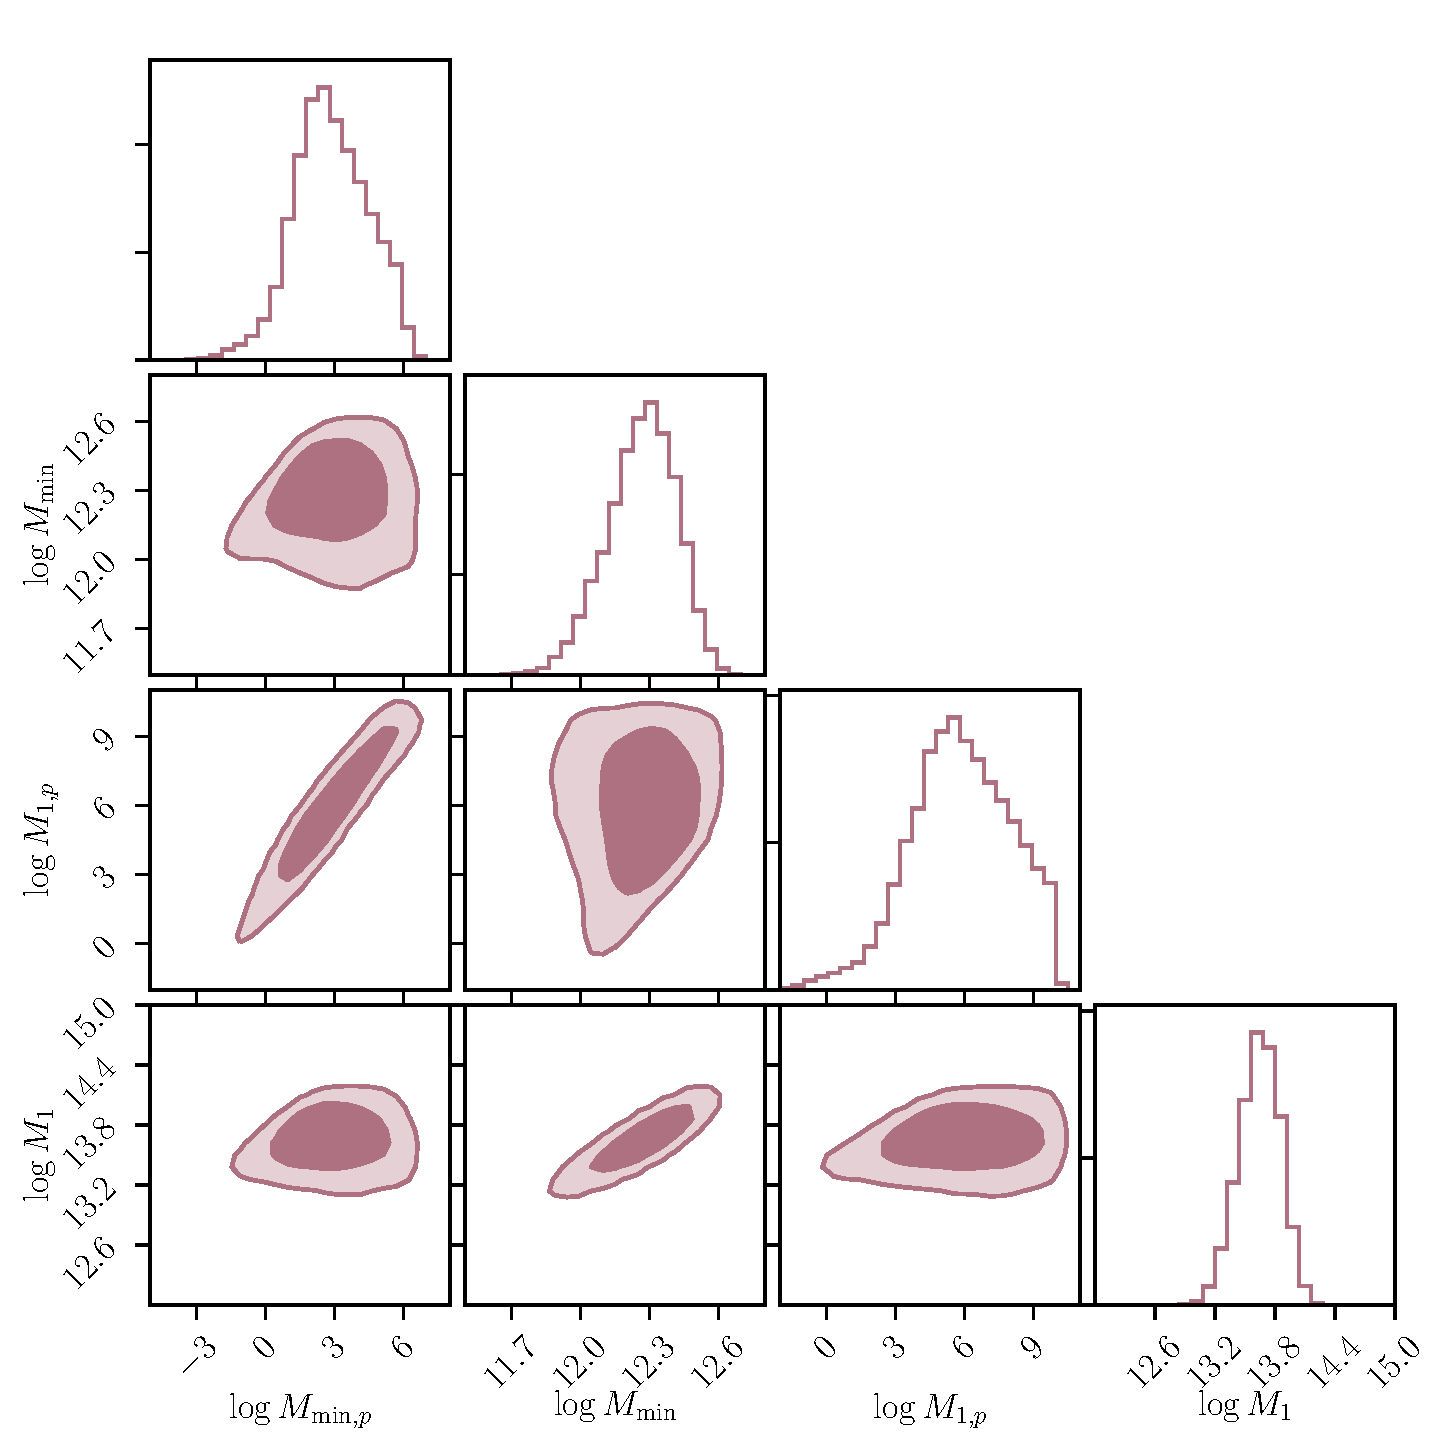
\includegraphics[width=0.95\textwidth]{figures/contours-Mmin-M1_mPk=HOD_fix=alpha-fc-sigmaM_HOD=zevol_fit=pz-shifts+prior=0p2-pz-widths+prior=0p2_fit=auto+cross_cosmo=const_cov=G+NG+SSC-LINBIAS_HOD-param=zfid_clfit=HOD-zevol.pdf}
\caption{Fiducial constraints on HOD parameters obtained in this work. The inner (outer) contour shows the $68 \%$ c.l. ($95 \%$ c.l.).}
\label{fig:constraints-fid-hod}
\end{center}
\end{figure}

\begin{figure}
\begin{center}
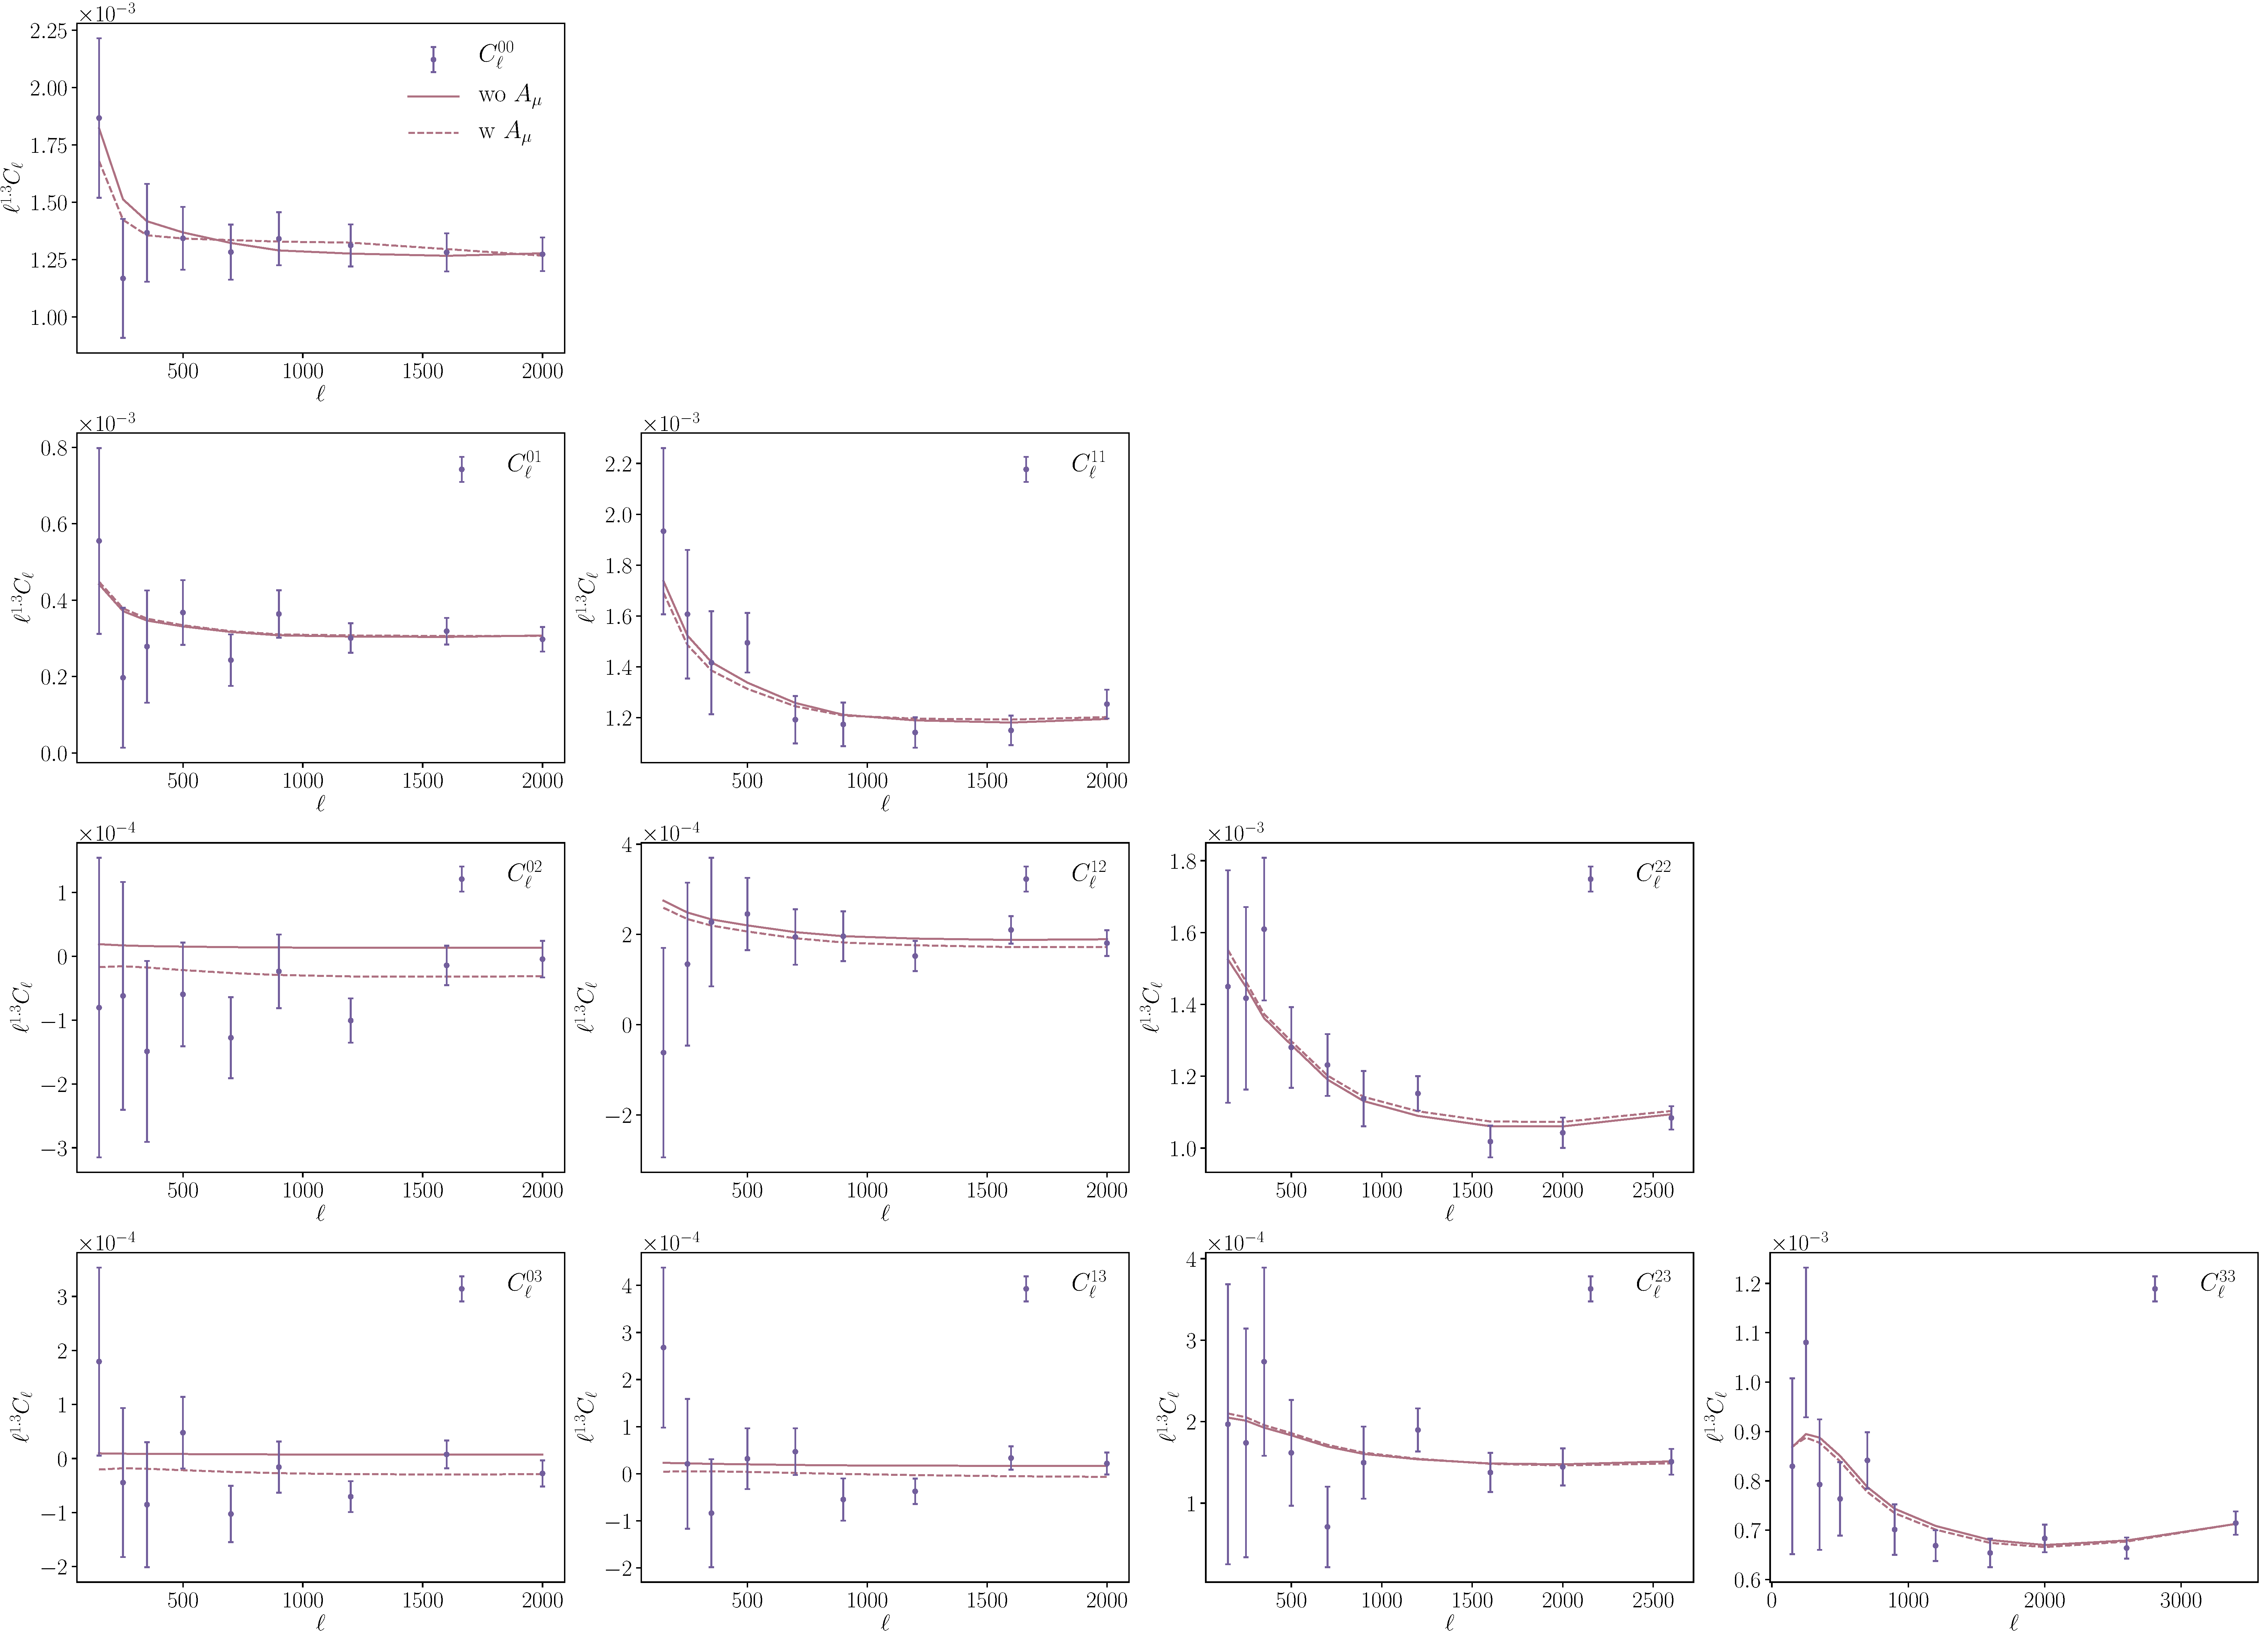
\includegraphics[width=0.95\textwidth]{figures/Cls-data-vs-best-fit_mPk=HOD_fix=alpha-fc-sigmaM_HOD=zevol_fit=pz-shifts+prior=0p2-pz-widths+prior=0p2_fit=auto+cross_cosmo=const_cov=G+NG+SSC-LINBIAS_HOD-param=zfid_clfit=HOD-zevol_no-mag-vs-mag.pdf}
\caption{Measured auto- and cross power spectra considered in our analysis. The solid lines show the theoretical predictions obtained from the best-fit model parameters obtained in a joint fit to both auto- and cross power spectra not allowing for magnification while the dashed lines show the theoretical predictions obtained allowing for a free magnification amplitude $A_{\mu}$.}
\label{fig:cls-best-fit}
\end{center}
\end{figure}

\begin{figure}
\begin{center}
\subfigure{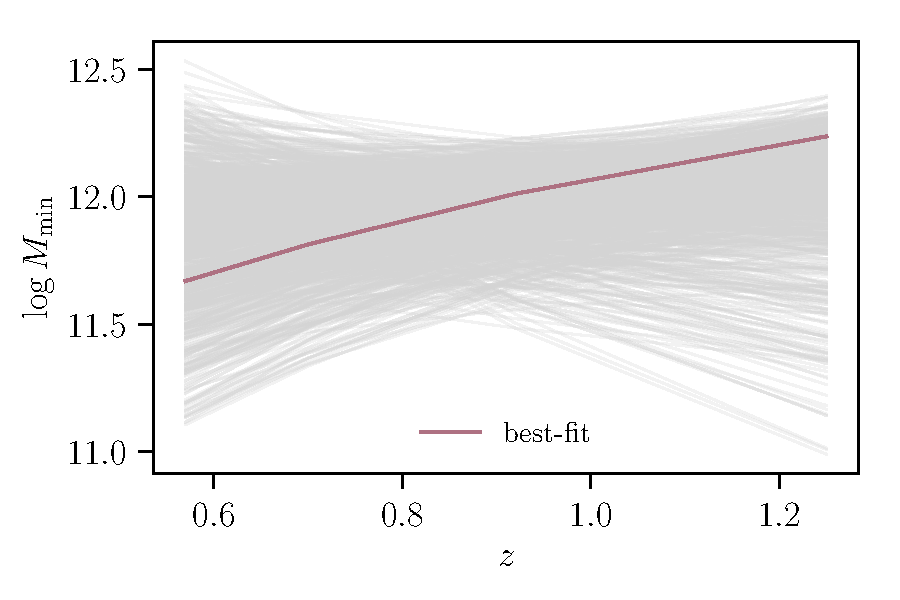
\includegraphics[width=0.49\textwidth]{figures/logM_min_z_dependence_mPk=HOD_fix=alpha-fc-sigmaM_HOD=zevol_fit=pz-shifts+prior=0p2-pz-widths+prior=0p2_fit=auto+cross_cosmo=const_cov=G+NG+SSC-LINBIAS_HOD-param=zfid_clfit=HOD-zevol_best-fit+random-draws.pdf}}
\subfigure{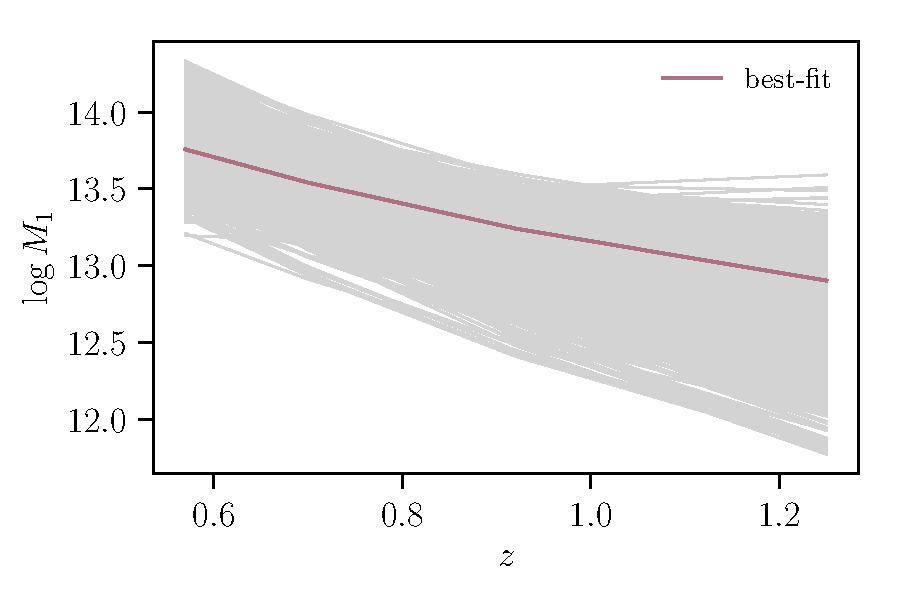
\includegraphics[width=0.49\textwidth]{figures/logM_1_z_dependence_mPk=HOD_fix=alpha-fc-sigmaM_HOD=zevol_fit=pz-shifts+prior=0p2-pz-widths+prior=0p2_fit=auto+cross_cosmo=const_cov=G+NG+SSC-LINBIAS_HOD-param=zfid_clfit=HOD-zevol_best-fit+random-draws.pdf}} 
\caption{Functional forms for $M_{\mathrm{min}}$ and $M_{1}$ derived from our best-fit theoretical model alongside the functions derived from 1000 random realizations of the MCMCs to illustrate the uncertainty.} 
\label{fig:hod-params-z-dep}
\end{center}
\end{figure}

\subsubsection{Robustness to modeling and data choices}

In order to test the robustness of our fiducial HOD constraints to implementation and data choices, we compare the constraints from several analysis variants, as described in the following. A summary of all robustness tests performed and the respective constraints on HOD parameters and extended models can be found in Tab.~\ref{tab:constraints_robustness}.

\begin{sidewaystable}
\caption{Parameter constraints and best-fit $\chi^{2}$ values obtained for all considered analysis variants. The number of degrees of freedom $\nu$ is estimated according to $\nu = N_{\mathrm{data}}-N_{\mathrm{param}}$. In the second column of the table, the values in brackets denote the $p$-values corresponding to the observed best-fit $\chi^{2}$. The uncertainties denote the $68 \%$ c.l..} \label{tab:constraints_robustness}
\begin{center}
\begin{tabular}{ccccccccc}
\hline\hline 
Analysis variant & $\sfrac{\chi^{2}}{\nu}$ & $M_{\mathrm{min}, p}$ & $M_{\mathrm{min}}$ & $M_{1, p}$ & $M_{1}$ & $A_{\mu}$ & $\Omega_{c}$ & $\sigma_{8}$ \\ \hline \Tstrut       
fiducial & $\sfrac{86.2}{80}$ $(0.30)$ & $-0.491\substack{+2.09 \\ -2.02}$ & $11.88\substack{+0.22 \\ -0.23}$ & $0.933\substack{+2.67 \\ -2.56}$ & $13.08\substack{+0.27 \\ -0.28}$ & - & - & - \\
auto & $\sfrac{19.2}{25}$ $(0.79)$ & $-0.886\substack{2.19 \\ -2.17}$ & $11.82 \pm 0.28$ & $0.368\substack{+2.67 \\ -2.64}$ & $13.00 \pm 0.33$  & - & - & - \\
G cov & $\sfrac{87.2}{80}$ $(0.27)$ & $-0.675\substack{+2.11 \\ -2.08}$ & $11.88\substack{+0.23 \\ -0.24}$ & $0.70\substack{+2.67 \\ -2.61}$ & $13.08\substack{+0.28 \\ -0.29}$ & - & - & - \\
G+SSC cov & $\sfrac{86.2}{80}$ $(0.30)$ & $-0.433\substack{+1.96 \\ -1.90}$ & $11.89 \pm 0.20$ & $0.982\substack{+2.55 \\ -2.44}$ & $13.09\substack{+0.24 \\ -0.25}$ & - & - & - \\
no $z_{w, i}$ & $\sfrac{88.0}{84}$ $(0.36)$ & $-0.855\substack{+0.645 \\ -0.652}$ & $11.87 \pm 0.11$ & $0.327\substack{+0.889 \\ -0.900}$ & $13.07 \pm 0.15$ & - & - & - \\
no $z_{w, i}, \Delta z_{i}$ & $\sfrac{95.2}{88}$ $(0.28)$ & $-1.09\substack{+0.624 \\ -0.771}$ & $11.78 \pm 0.13$ & $-0.108\substack{+0.727 \\ -0.940}$ & $12.93 \pm 0.16$ & - & - & - \\
bins = 0, 1, 2 & $\sfrac{44.4}{43}$ $(0.41)$ & $-0.354\substack{+2.34 \\ -2.25}$ & $11.88\substack{+0.22 \\ -0.23}$ & $0.624\substack{+2.87 \\ -2.75}$ & $13.09\substack{+0.27 \\ -0.28}$ & - & - & - \\
bins = 1, 2, 3 & $\sfrac{44.4}{46}$ $(0.54)$ & $1.20\substack{+2.88 \\ -2.97}$ & $11.97\substack{+0.31 \\ -0.36}$ & $3.49\substack{+4.16 \\ -4.08}$ & $13.19\substack{+0.42 \\ -0.39}$ & - & - & - \\
pz = \texttt{Ephor\_AB} & $\sfrac{93.6}{80}$ $(0.14)$ & $0.270\substack{+2.05 \\ -1.88}$ & $12.14\substack{+0.19 \\ -0.17}$ & $1.82\substack{+2.87 \\ -2.59}$ & $13.39\substack{+0.24 \\ -0.23}$ & - & - & - \\
pz = \texttt{Ephor} & $\sfrac{107.2}{80}$ $(0.023)$ & $0.895\substack{+1.97 \\ -2.03}$ & $12.15 \pm 0.17$ & $2.64\substack{+2.71 \\ -2.80}$ & $13.40\substack{+0.23 \\ -0.22}$ & - & - & - \\
pz = \texttt{DEmP} & $\sfrac{105.4}{80}$ $(0.031)$ & $0.616\substack{+1.90 \\ -1.88}$ & $12.07\substack{+0.17 \\ -0.16}$ & $2.29\substack{+2.59 \\ -2.55}$ & $13.30\substack{+0.22 \\ -0.21}$ & - & - & - \\
pz = \texttt{FRANKEN-Z} & $\sfrac{90.8}{80}$ $(0.19)$ & $0.0421\substack{+1.97 \\ -1.76}$ & $12.12\substack{+0.18 \\ -0.16}$ & $1.41\substack{+2.75 \\ -2.44}$ & $13.38\substack{+0.23 \\ -0.22}$ & - & - & - \\
fiducial magn. & $\sfrac{72.8}{80}$ $(0.70)$ & $-0.358\substack{+2.56 \\ -2.32}$ & $11.94\substack{+0.21 \\ -0.22}$ & $1.04\substack{+3.32 \\ -2.97}$ & $13.16\substack{+0.26 \\ -0.27}$  & - & - & - \\
fit magn., auto+cross & $\sfrac{69.0}{79}$ $(0.78)$ & $-1.78\substack{+2.14 \\ -2.35}$ & $11.79\substack{+0.26 \\ -0.27}$ & $-0.724\substack{+2.60 \\ -2.74}$ & $12.98\substack{+0.30 \\ -0.31}$  & $2.18 \pm 0.74$ & - & - \\
fit magn., auto & $\sfrac{19.4}{24}$ $(0.73)$ & $-0.844\substack{+2.29 \\ -2.17}$ & $11.81 \pm 0.26$ & $0.409\substack{+2.80 \\ -2.65}$ & $12.98 \pm 0.31$  & $0.627\substack{+2.71 \\ -2.61}$ & - & - \\
fit cosmo & $\sfrac{84.4}{78}$ $(0.29)$ & $0.0143\substack{+2.72 \\ -2.53}$ & $11.79\substack{+0.27 \\ -0.24}$ & $1.63\substack{+3.44 \\ -3.20}$ & $12.96\substack{+0.36 \\ -0.35}$  & - & $0.237 \pm 0.025$ & $0.807\substack{+0.149 \\ -0.143}$ \\
 \hline \hline
\end{tabular}
\end{center}
\end{sidewaystable}

As discussed above, our fiducial constraints are derived from a joint fit to both auto- and cross power spectra. However, cross correlations between redshift bins are susceptible to photometric redshift errors, such as outliers. In order to test for systematics affecting the cross-correlations, we therefore test the consistency of the auto- and cross power spectra by comparing the constraints obtained using only auto power spectra to those obtained when jointly fitting auto- and cross power spectra. Fig.~\ref{fig:constraints-cov=G+NG+SSC-vs-cov=G-vs-cov=G+SSC-vs-fit=auto} shows the comparison between our fiducial HOD constraints and those obtained from auto power spectra alone. As can be seen, the constraints from auto power spectra and auto- and cross power spectra agree very well with each other, suggesting that uncertainties in photometric redshifts do not significantly affect the cross-correlations measured in our analysis. Furthermore, we see that the constraining power on HOD parameters is unaffected by including the cross power spectra. As a final consistency check between auto- and cross power spectra we test how well the auto power spectra predict the cross power spectra. To this end we compute the $\chi^{2}$ between the observed auto- and cross power spectra and the theoretical predictions derived from auto power spectra only. As we will discuss below, the auto power spectra cannot constrain the photo-$z$ systematics parameters and we therefore fix $z_{w, i} = 0, \Delta z_{i} = 0$ for this test. We find $\chi^{2} = 95.3$, which is practically equivalent to the best-fit $\chi^{2}$ obtained when fitting both auto- and cross power spectra without accounting for photo-$z$ systematics (see Tab.~\ref{tab:constraints_robustness}). This shows that the auto power spectra are able to predict the cross power spectra and provides further confirmation of their consistency. 

An important part of our data model is the analytical covariance matrix described in Sec.~\ref{sssec:methods.theory.covar}. In order to test the impact of the non-Gaussianity of the covariance on our results, we compare the HOD constraints obtained accounting for Gaussian (G) and Gaussian and SSC contributions (G+SSC) to our fiducial constraints, which include Gaussian, SSC and non-Gaussian contributions. As can be seen from Fig.~\ref{fig:constraints-cov=G+NG+SSC-vs-cov=G-vs-cov=G+SSC-vs-fit=auto}, these constraints agree very well with each other. The constraints from the G and the G+SSC case yield almost identical constraints, which is expected due to the suppression of the SSC contribution by the number density correction (c.f. Sec.~\ref{ssec:results.covariance}). Accounting for all non-Gaussian contributions to the covariance results in slightly broadened but consistent constraints. Comparing to Fig.~\ref{fig:covariance-contributions}, this is probably due to the fact that these corrections only affect the lowest redshift bins at small angular scales and therefore do not have a significant impact when computing constraints from all power spectra. Finally, from Tab.~\ref{tab:constraints_robustness} we see that the reduced $\chi^{2}$s of the data slightly increase as we account for less contributions to the total covariance, as expected. However, we find an acceptable goodness of fit, even when only accounting for the Gaussian covariance.

\begin{figure}
\begin{center}
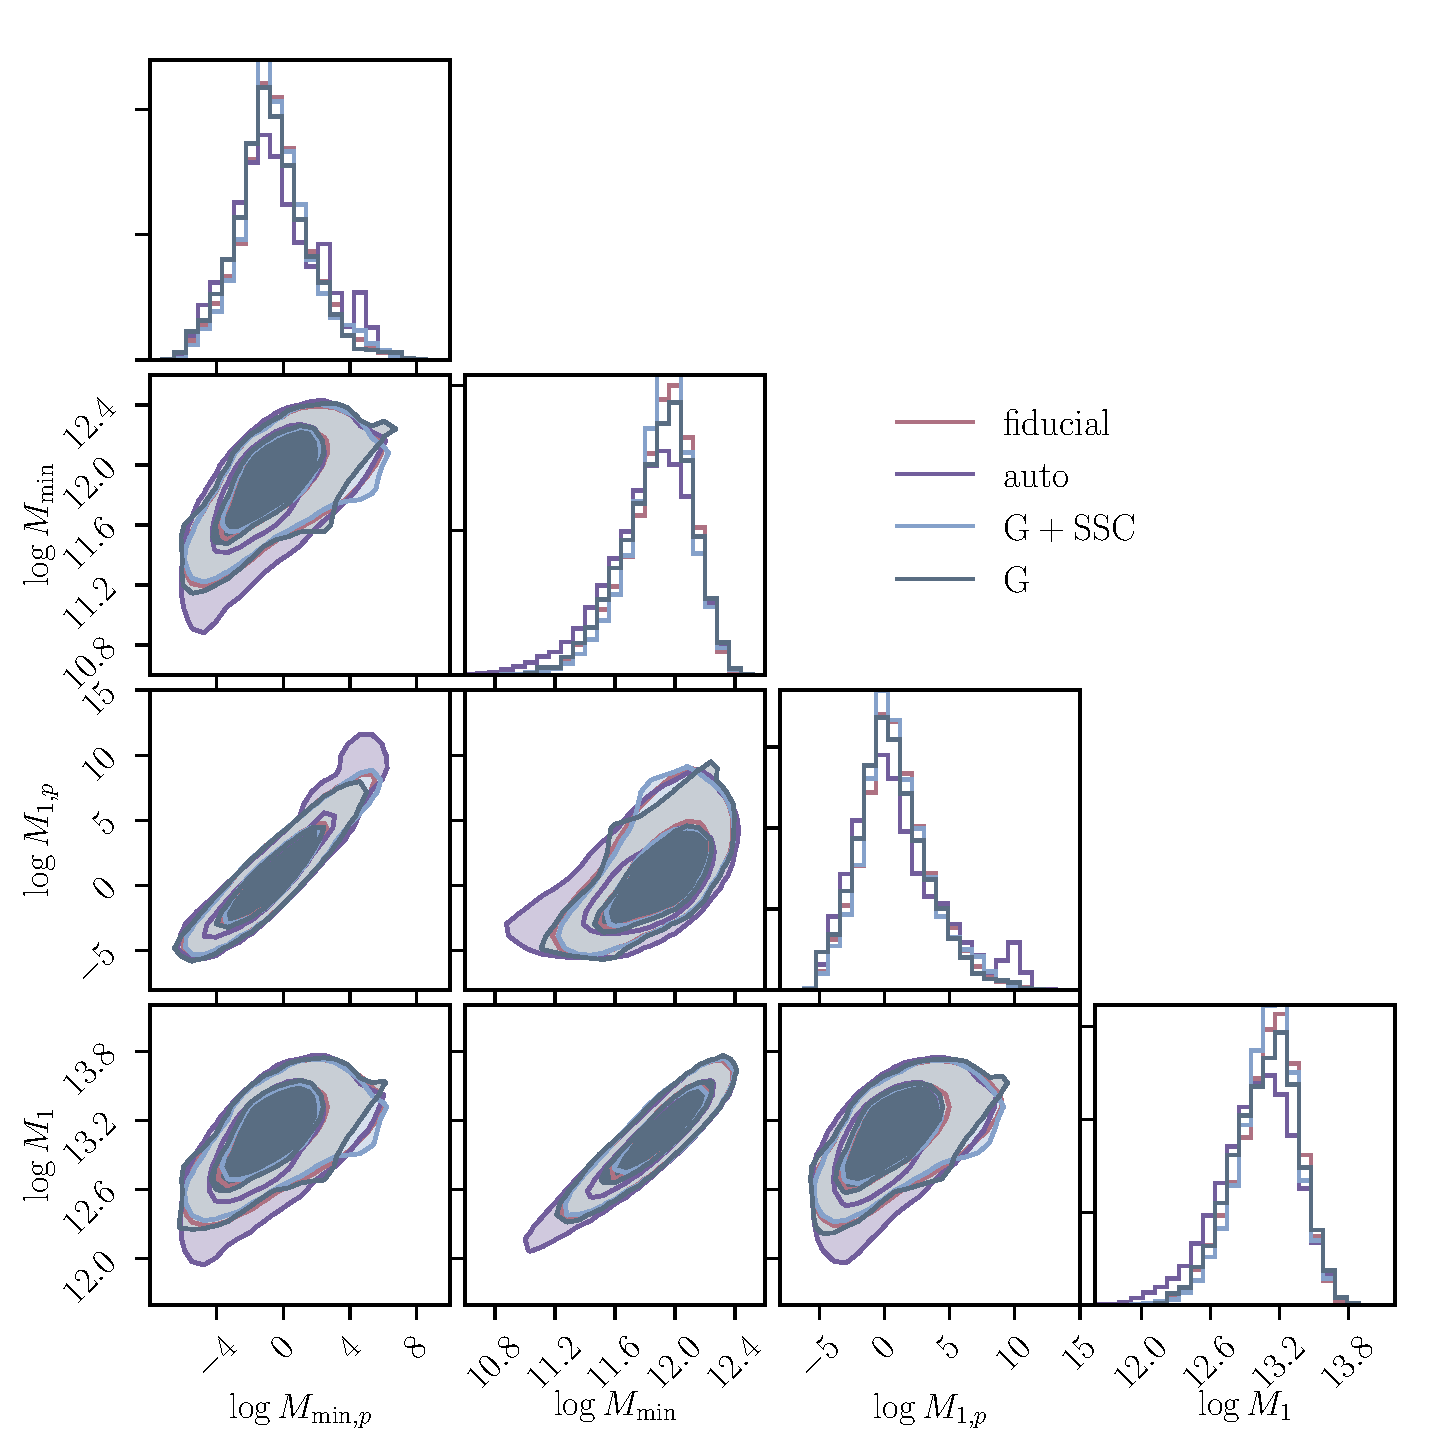
\includegraphics[width=0.95\textwidth]{figures/contours-Mmin-M1_mPk=HOD_fix=alpha-fc-sigmaM_HOD=zevol_fit=pz-shifts-pz-widths+prior=0p2_fit=auto+cross_cosmo=const_HOD-param=zfid_clfit=HOD-zevol_cov=G+NG+SSC-vs-fit=auto-vs-cov=G-vs-cov=G+SSC.pdf}
\caption{Comparison of our fiducial constraints on HOD parameters to those obtained from auto power spectra alone, accounting only for Gaussian and Gaussian and SSC contributions to the covariance matrix. The inner (outer) contour shows the $68 \%$ c.l. ($95 \%$ c.l.).}
\label{fig:constraints-cov=G+NG+SSC-vs-cov=G-vs-cov=G+SSC-vs-fit=auto}
\end{center}
\end{figure}

\subsubsection{Robustness to photometric redshift uncertainties}

One of the most important potential systematics in photometric galaxy clustering analyses are photometric redshift uncertainties and we therefore test the stability of our results to photo-$z$s in several different ways, as described in detail below. 

In Fig.~\ref{fig:constraints-pz-syst-auto+cross-vs-auto}, we show the constraints on photometric redshift systematics parameters derived in our fiducial analysis. We find that the data cannot separately constrain the mean shift parameters $\Delta z_{i}$, as opposed to pairwise differences between those. We therefore show the constraints in terms of the reparametrized parameters $\Sigma_{i} \Delta z_{i}, \Delta z_{1} - \Delta z_{0}, \Delta z_{2} - \Delta z_{1}, \Delta z_{3} - \Delta z_{2}$, which denote the sum of the $\Delta z_{i}$ and their pairwise differences respectively. While $\Sigma_{i} \Delta z_{i}$ and $z_{w, i}$ are largely unconstrained, we find that we can constrain the three pairwise differences $\Delta z_{i} - \Delta z_{j}$ to within $\sigma_{\Delta z_{i} - \Delta z_{j}} \approx 0.023$ ($68 \%$ c.l.). This means that the data do not allow constraining the absolute position of each redshift bin, but are quite sensitive to their relative positions.

It is instructive to investigate which part of the data drives the constraints on photometric redshift systematics. To this end we compare the constraints obtained using auto power spectra only to those obtained from auto- and cross power spectra (our fiducial case). As can be seen from Fig.~\ref{fig:constraints-pz-syst-auto+cross-vs-auto}, we find that the auto power spectra do not constrain the photo-$z$ systematics parameters $\Delta z_{i} - \Delta z_{j}$, as opposed to the combination of auto- and cross power spectra. This shows that the cross correlations drive the constraints on photometric redshift systematics and are thus essential for jointly constraining redshift systematics and astrophysical/cosmological parameters from galaxy clustering data.

In order to test the impact of photometric redshift uncertainties on our fiducial HOD constraints, we compare them to those obtained when separately fixing $z_{w, i} = 0$ and $z_{w, i} = 0, \Delta z_{i} = 0$. The results are shown in Fig.~\ref{fig:constraints-hod-pz-shifts-pz-widths-vs-pz-shifts-vs-no-pz-shifts}. As expected, we find that the constraints on HOD parameters successively weaken as we include more freedom in the photo-$z$ error model. However, as can be seen both from Fig.~\ref{fig:constraints-hod-pz-shifts-pz-widths-vs-pz-shifts-vs-no-pz-shifts} and Tab.~\ref{tab:constraints_robustness}, the constraints obtained in the three cases agree very well. In addition, we find acceptable $\chi^{2}$ values both for the model with $z_{w, i} = 0$ and $z_{w, i} = 0, \Delta z_{i} = 0$. This suggests that our fiducial HOD constraints are robust to photo-$z$ uncertainties in the COSMOS 30-band catalog, as parametrized through Eq.~\ref{eq:photo-z-model}. 

As described in Sec.~\ref{ssec:methods.nz}, our fiducial constraints use the redshift distributions derived using COSMOS 30-band data \cite{2016ApJS..224...24L}. There are several potential caveats associated with this approach. First, the   photometric redshift accuracy decreases significantly for objects in the COSMOS 30-band catalog with $z > 1.4$ and second, the fraction of catastrophic outliers at faint magnitudes ($23 \leq$ \texttt{i+} $\leq 25$) is estimated to be around $6-10 \%$ \cite{2016ApJS..224...24L}. We expect the highest redshift bin to be mostly affected by decreasing photometric redshift accuracy. However, as noted in \cite{Joudaki:2019}, catastrophic outliers that are erroneously assigned to too low redshifts are more likely to fall into our sample than outliers assigned to too high redshifts. Therefore, the lowest redshift bin in particular might also be affected by photometric redshift errors \an{not sure this is the reason for which Jeff asked us to remove the low-z bin...}. In order to test the robustness of our results to photometric redshift uncertainties at low and high redshifts, we compute parameter constraints separately neglecting the high and low redshift bin and all its cross-correlations. The results of these two analyses are shown alongside our fiducial constraints in Fig.~\ref{fig:constraints-fit-bins=0+1+2+3-vs-fit-bins=0+1+2-vs-fit-bins=1+2+3}. As can be seen, we find all constraints to agree well with each other. This suggests that our analysis is robust against photometric redshift uncertainties in the COSMOS 30-band catalog affecting the lowest or highest of our redshift bins. 

We have also investigated the impact of a secondary mode in the redshift distribution for the first tomographic bin. This secondary peak contains 5\% of galaxies and peaks around $z\sim 2.5$ (hence cannot be seen in Figure \ref{fig:nzs}). To investigate the impact of this mode, we manually excise it from redshift distribution and calculate the resulting change in $\Delta \chi^2\sim 0.1$. This indicates that the effect of this bump is to small to be statistically significant. We therefore do not need to worry whether it is real or an artifact of photometric redshift inference.  \as{Fix numbers once Sarah gets back}

 \begin{figure}
\begin{center}
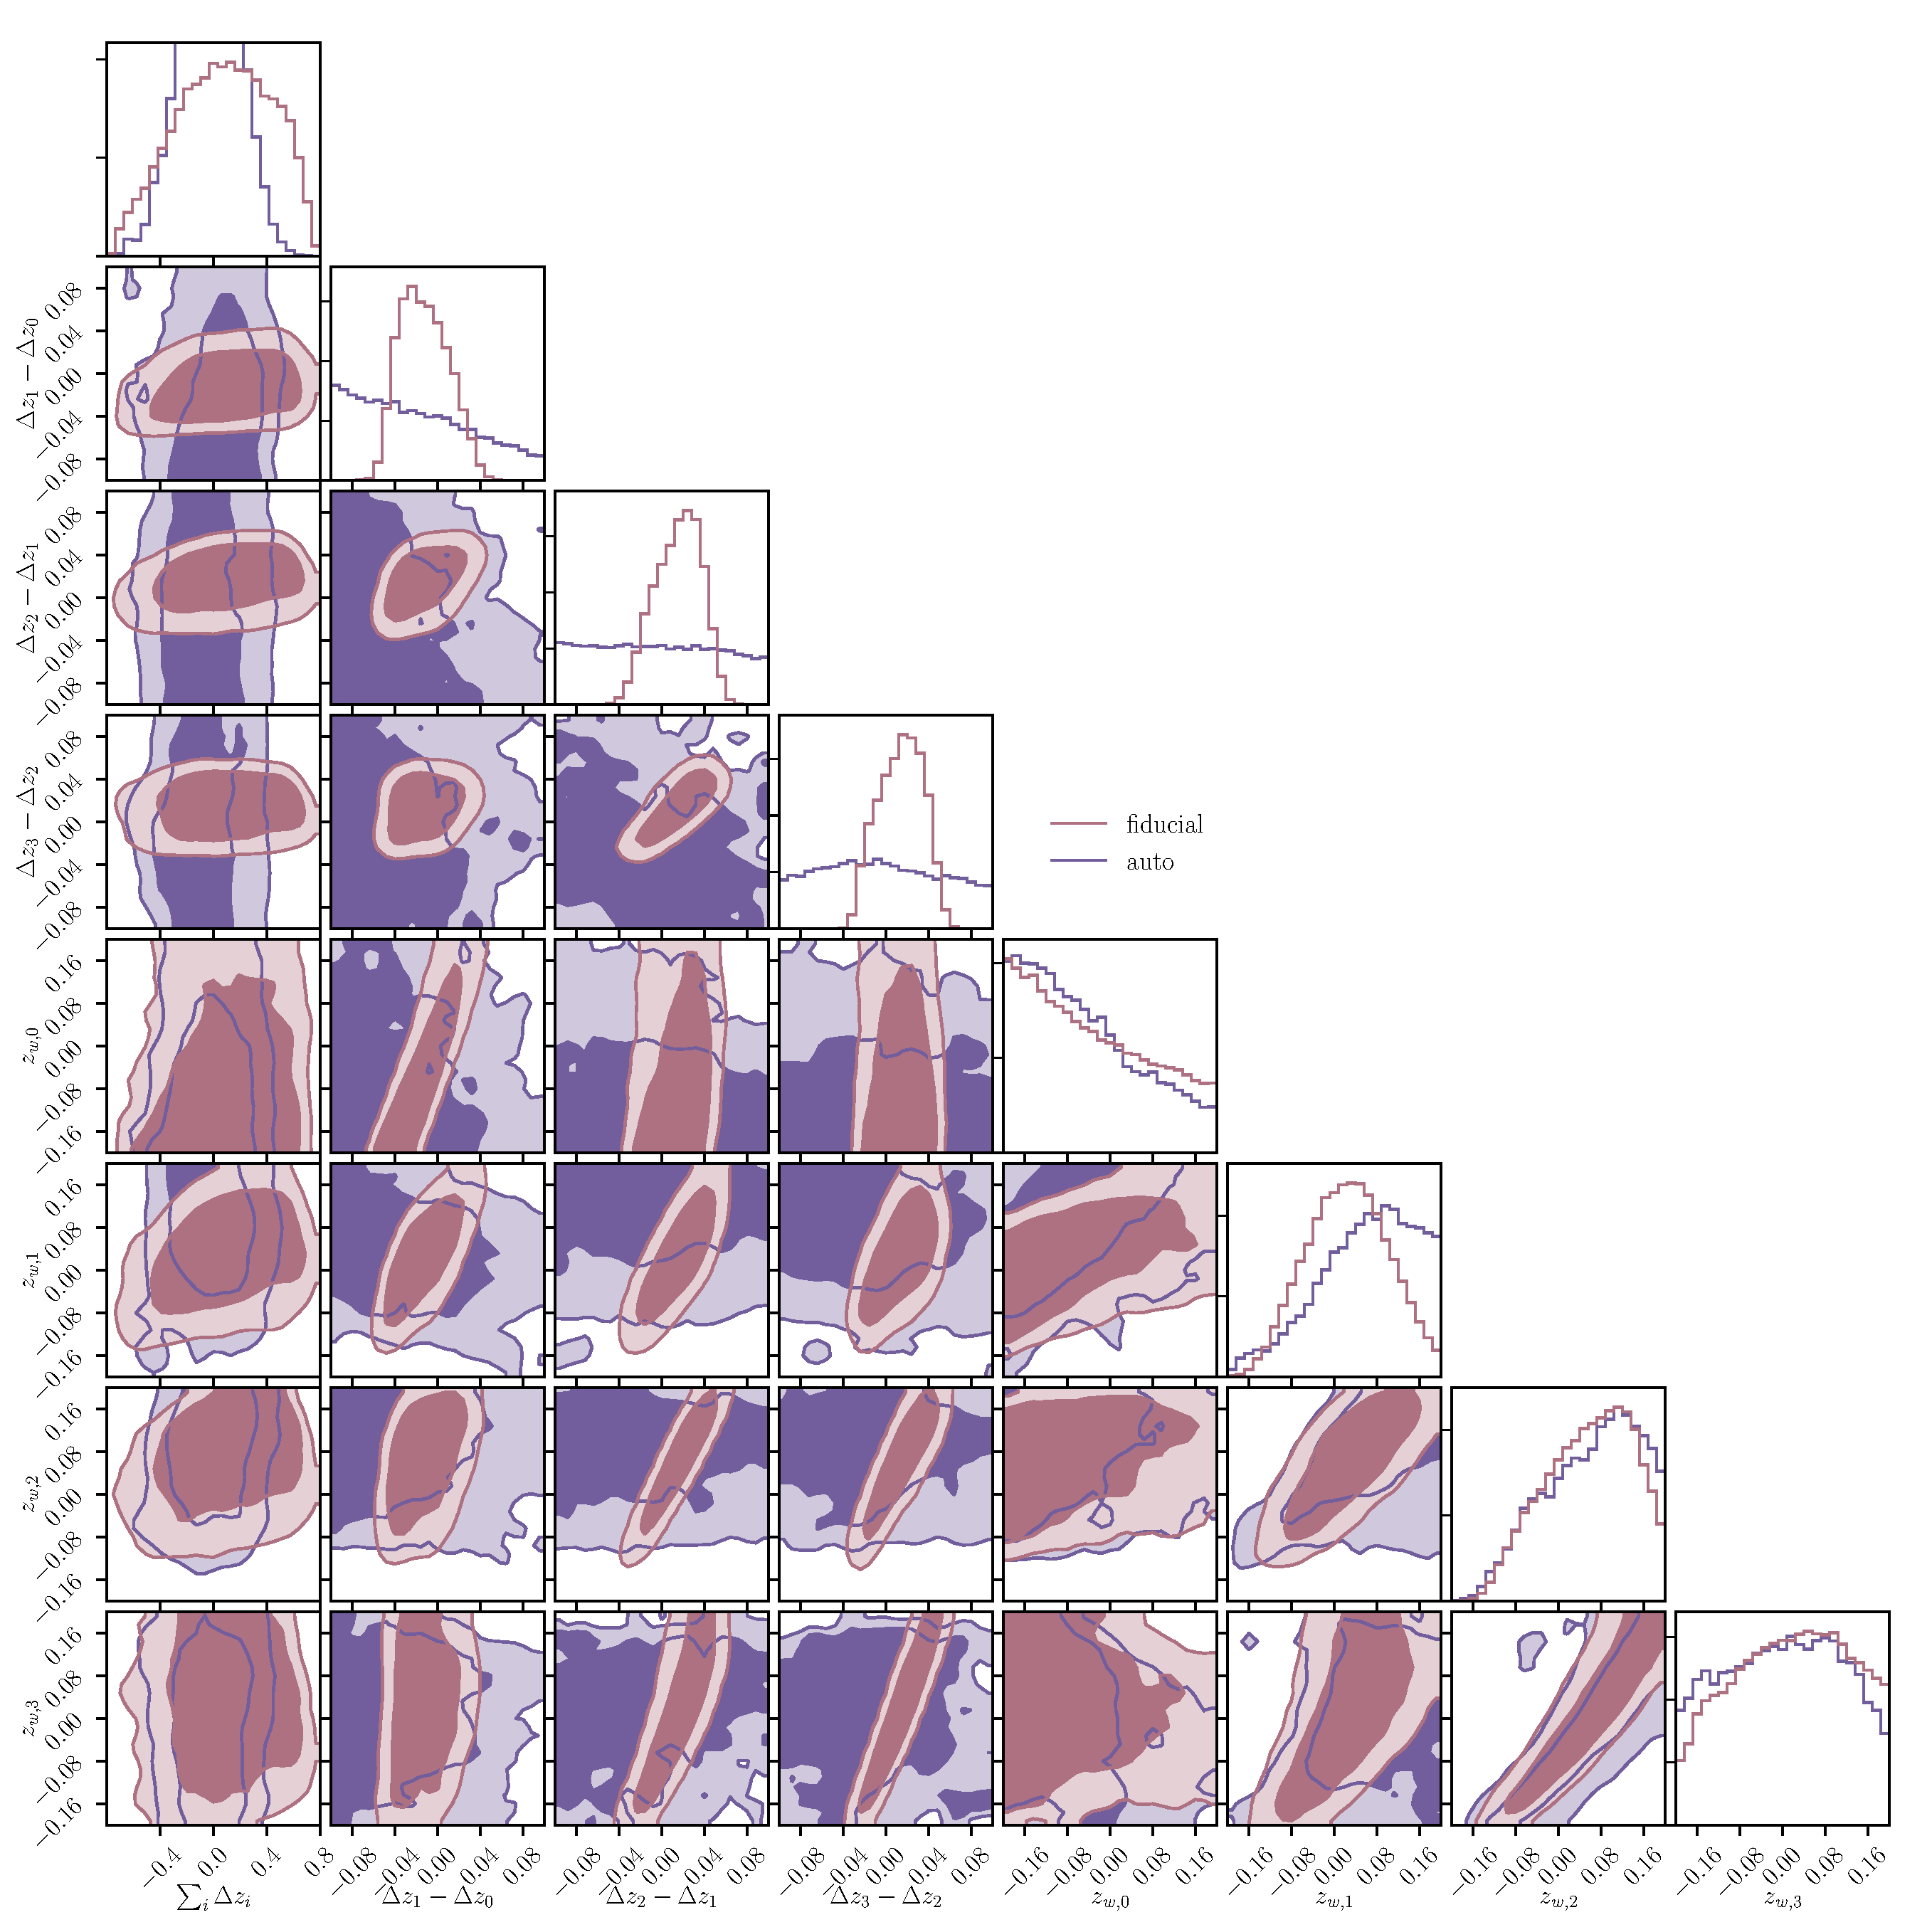
\includegraphics[width=0.95\textwidth]{figures/contours-pz-syst_mPk=HOD_fix=alpha-fc-sigmaM_HOD=zevol_fit=pz-shifts+prior=0p2-pz-widths+prior=0p2_cosmo=const_cov=G+NG+SSC-LINBIAS_HOD-param=zfid_clfit=HOD-zevol_fit=auto+cross-vs-fit=auto.pdf}
\caption{Comparison of our fiducial constraints on photo-$z$ systematics parameters to those obtained from auto power spectra alone. The inner (outer) contour shows the $68 \%$ c.l. ($95 \%$ c.l.).}
\label{fig:constraints-pz-syst-auto+cross-vs-auto}
\end{center}
\end{figure}

 \begin{figure}
\begin{center}
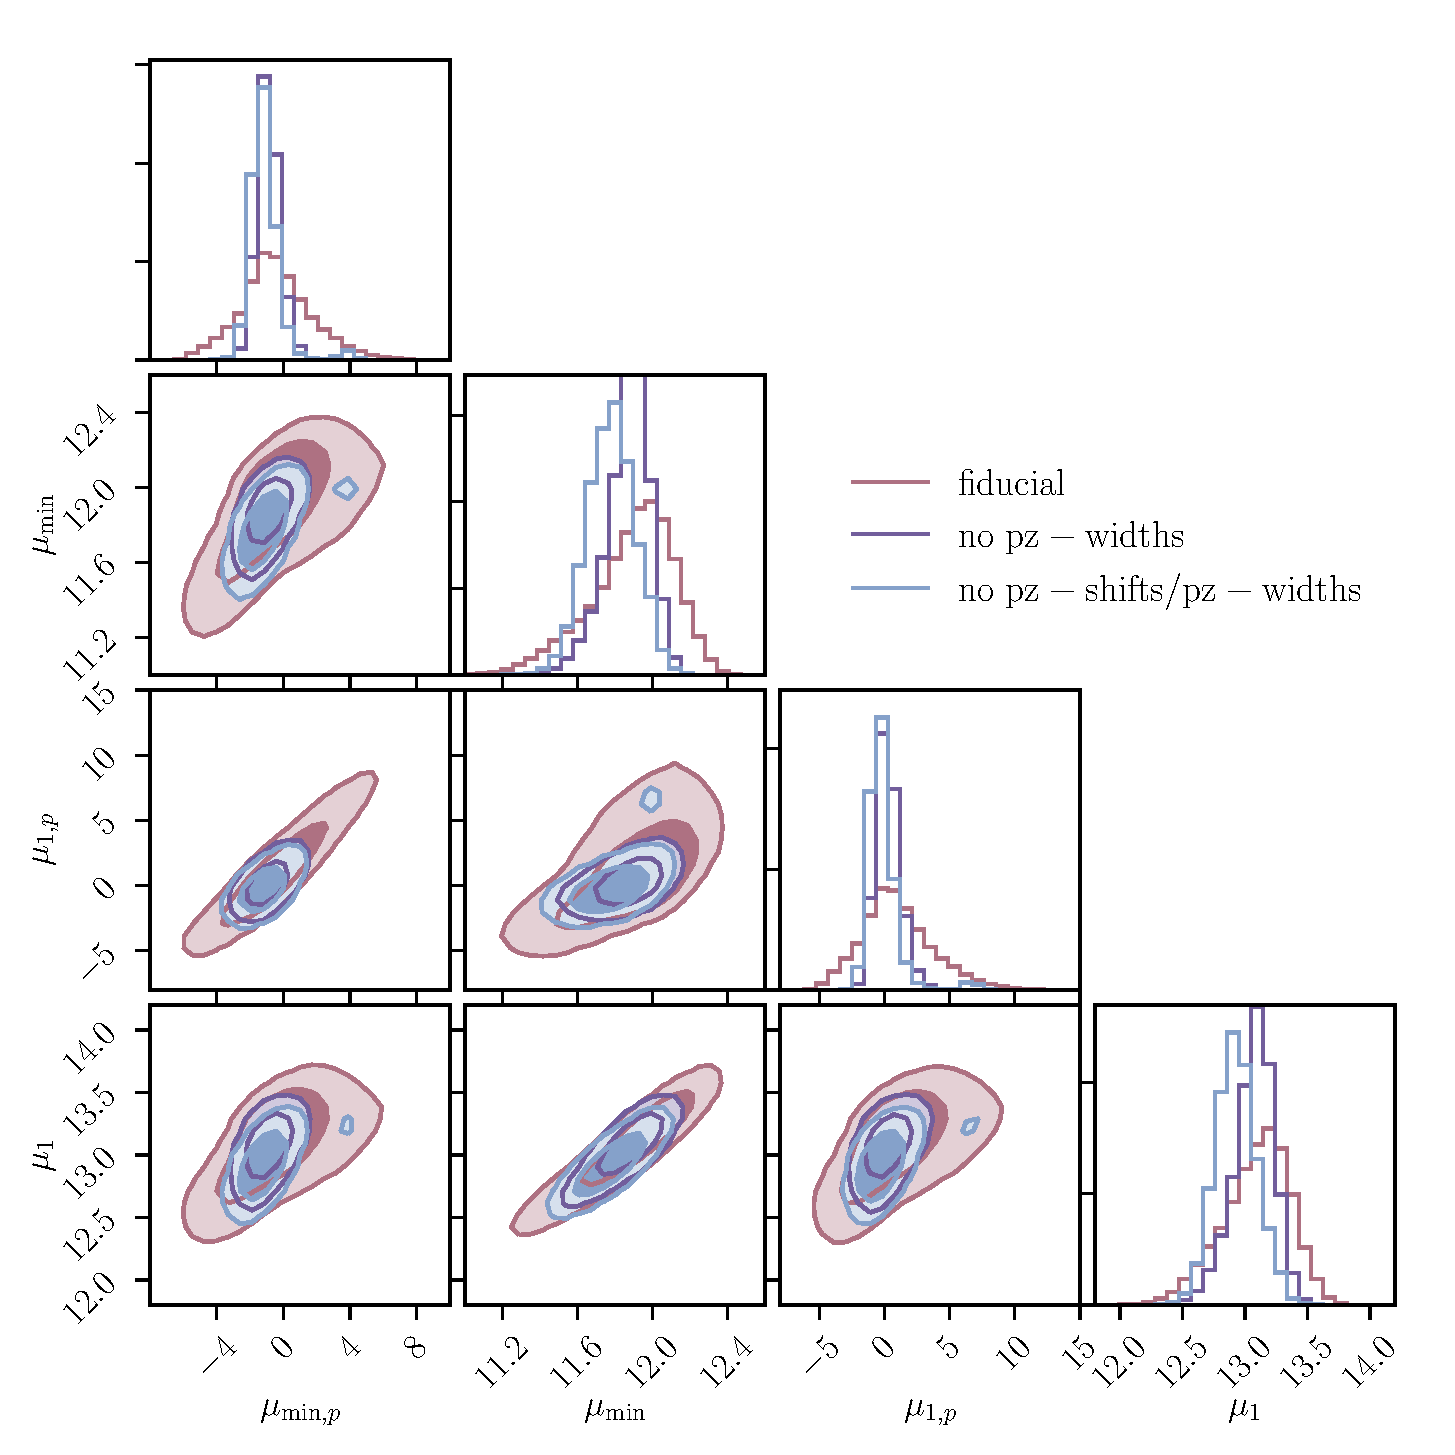
\includegraphics[width=0.95\textwidth]{figures/contours-Mmin-M1_mPk=HOD_fix=alpha-fc-sigmaM_HOD=zevol_fit=pz-shifts-pz-widths+prior=0p2_fit=auto+cross_cosmo=const_cov=G+NG+SSC-LINBIAS_HOD-param=zfid_clfit=HOD-zevol_fit=pz-shifts+widths-vs-fit=pz-shifts-vs-no-pz-shifts.pdf}
\caption{Comparison of our fiducial HOD constraints to those obtained setting $z_{w, i} = 0$ and $z_{w, i} = 0, \Delta z_{i} = 0$. The inner (outer) contour shows the $68 \%$ c.l. ($95 \%$ c.l.).}
\label{fig:constraints-hod-pz-shifts-pz-widths-vs-pz-shifts-vs-no-pz-shifts}
\end{center}
\end{figure}

\begin{figure}
\begin{center}
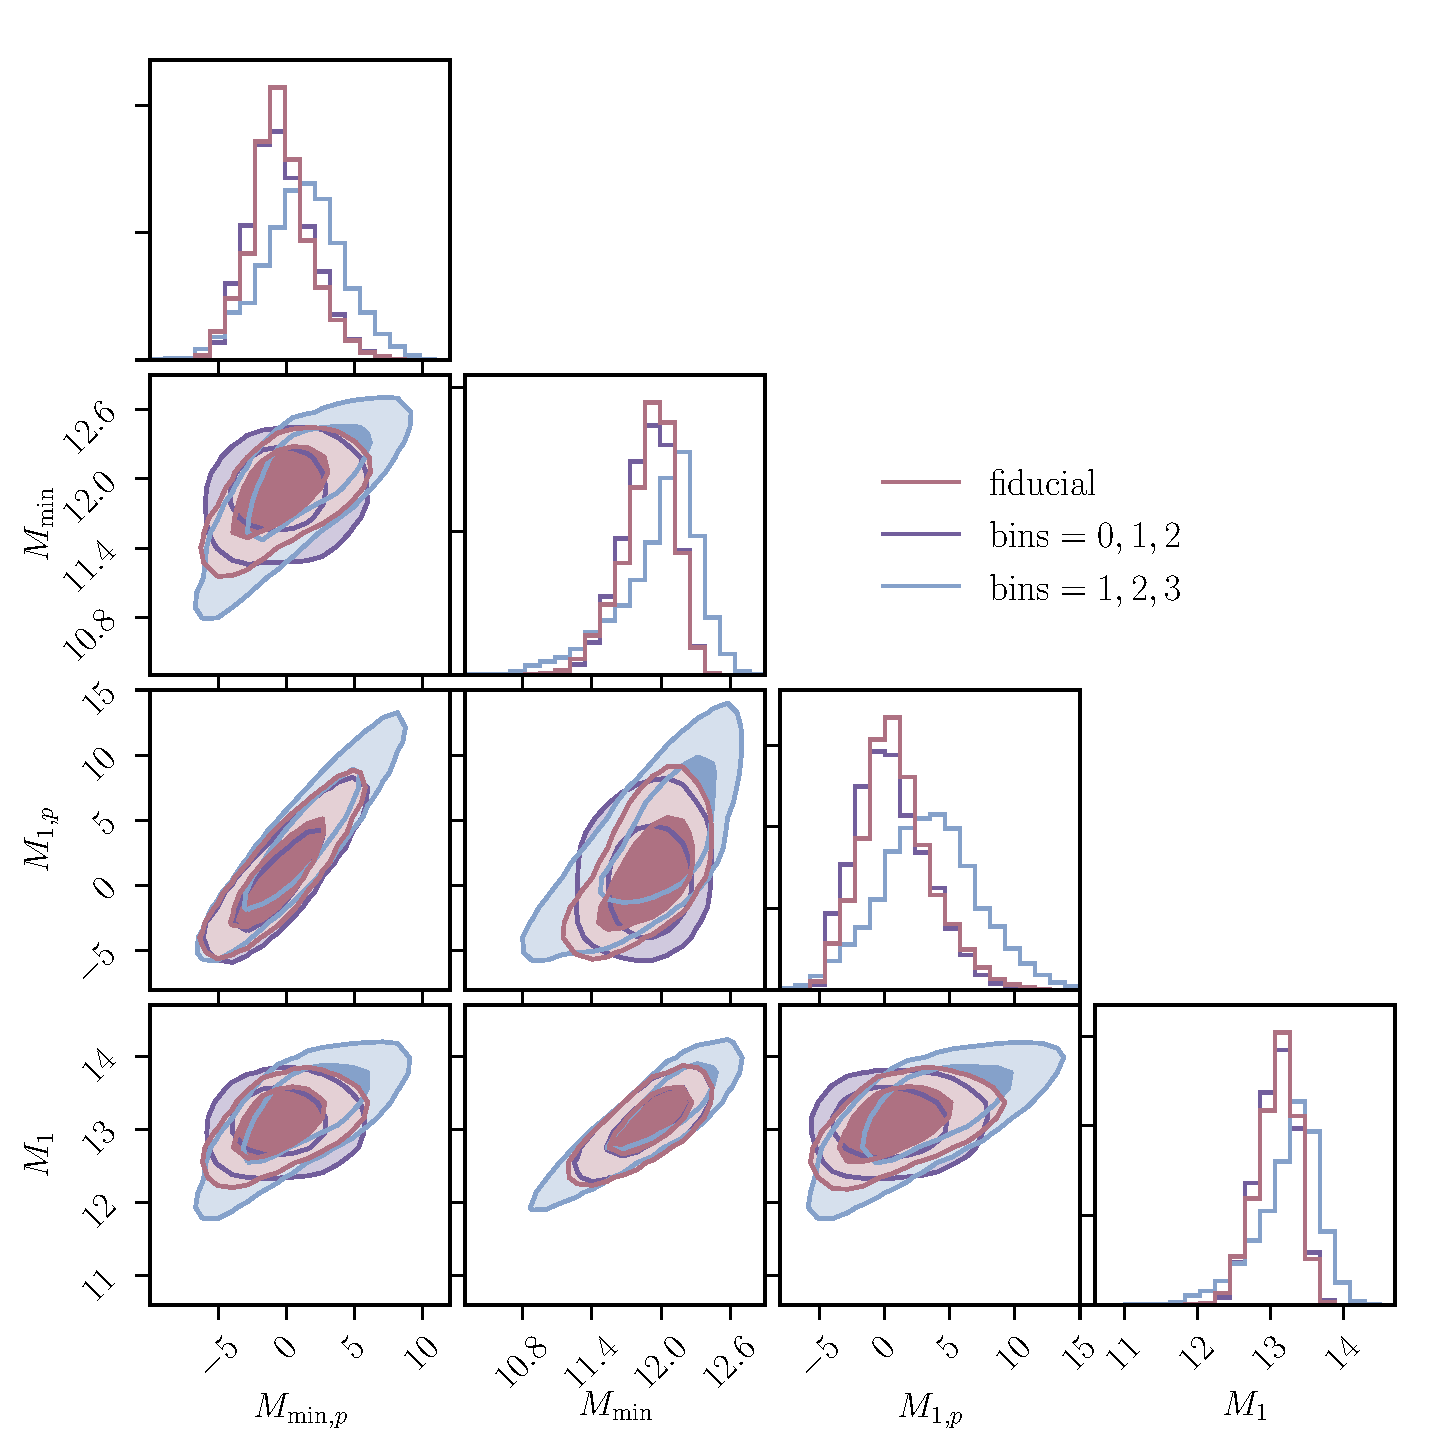
\includegraphics[width=0.95\textwidth]{figures/contours-Mmin-M1_mPk=HOD_fix=alpha-fc-sigmaM_HOD=zevol_fit=pz-shifts-pz-widths+prior=0p2_fit=auto+cross_cosmo=const_HOD-param=zfid_clfit=HOD-zevol_fit-bins=0+1+2+3-vs-fit-bins=0+1+2-vs-fit-bins=1+2+3.pdf}
\caption{Comparison of our fiducial constraints on HOD parameters to those obtained from the three lowest redshift bins and their cross correlations and those obtained from the three highest bins and their cross correlations. The inner (outer) contour shows the $68 \%$ c.l. ($95 \%$ c.l.).}
\label{fig:constraints-fit-bins=0+1+2+3-vs-fit-bins=0+1+2-vs-fit-bins=1+2+3}
\end{center}
\end{figure}

As a last test of robustness against photometric redshift errors, we compare our fiducial constraints to those obtained with the photo-$z$ codes \texttt{Ephor\_AB}, \texttt{Ephor}, \texttt{DEmP} and \texttt{FRANKEN-Z}, as provided by the HSC Collaboration \cite{2018PASJ...70S...9T}. In analogy to our fiducial analysis, we use the photometric redshift error model given in Eq.~\ref{eq:photo-z-model} for each photo-$z$ code. The comparison of the constraints on HOD and photo-$z$ systematics parameters obtained for the five different methods are shown in Figures \ref{fig:constraints-HOD-fit-pz-shifts+pz-widths-pz-methods} and \ref{fig:constraints-pz-syst-fit-pz-shifts+pz-widths-pz-methods}. As can be seen, the constraints on HOD parameters from all codes are in very good agreement, while we see some discrepancies between the constraints on photometric redshift systematics parameters, especially between $z_{w, 3}$ and $\Delta z_{3} - \Delta z_{2}$. However, these differences are not unexpected as these redshift distributions differ in means and shapes and are therefore not required to give consistent constraints on photo-$z$ systematics parameters. 

Even though the photo-$z$ error model given in Eq.~\ref{eq:photo-z-model} leads to consistent constraints on HOD parameters from all photo-$z$ methods considered, there is no guarantee that it is flexible enough to capture all redshift distribution differences important for galaxy clustering statistics. We investigate this by comparing the auto power spectra for a fixed HOD model obtained when forcing the five redshift distributions to have approximately the same means and widths. We find that the resulting power spectra exhibit significant differences, which suggests that features in the redshift distribution beyond mean and width can significantly impact observed galaxy clustering power spectra. In our case, accounting for uncertainties in means and widths gives consistent constraints on HOD parameters and we therefore conclude that this error model is flexible enough to characterize photo-$z$ uncertainties in the present case. However, this will probably cease to be true for future photometric clustering analyses (e.g. using LSST data) and suggests that these data sets will have to be analyzed accounting for the full uncertainty on the shape of the photometric redshift distributions.

In order to further illustrate the effects of an incomplete photo-$z$ error model, we perform two additional analyses in which we compare the constraints obtained from the five photo-$z$ methods setting $z_{w, i} = 0$ and $z_{w, i} = 0, \Delta z_{i} = 0$ respectively. In the former case we find that the values for the photo-$z$ systematics parameters $\Sigma_{i} \Delta z_{i}, \Delta z_{i} - \Delta z_{j}$ required by the different codes differ significantly, which leads to differences in both constraining power and constraints on HOD parameters. We especially find significant shifts in $M_{\mathrm{min}}$ and $M_{1}$ along their degeneracy direction. Investigating this further, we find that the observed differences in $\Delta z_{i}$ cannot be explained with the differences in mean redshift between the distributions derived using the five separate methods. In addition, we find that for the redshift distributions considered in this analysis, mean shifts mainly affect low redshift auto power spectra but have a significantly smaller impact on high redshift bins. Variations in the widths of the photo-$z$ distributions on the other hand, have a similar impact at low and high redshifts. This suggests that a photo-$z$ error model accounting only for mean shifts is too simplistic to account for the redshift distribution differences observed in this analysis. As borne out by the observed discrepancies in HOD constraints, our analysis is sensitive to these differences and we therefore need to extend the photo-$z$ error model. From the discussion above it follows that additionally accounting for variations in the widths of the distributions is sufficient, as this error model yields HOD constraints that are robust to changes in the photo-$z$ estimation method.

The discrepancies between HOD parameters derived from the five different methods become even stronger when we do not account for photo-$z$ uncertainties, as can be seen from Fig.~\ref{fig:constraints-HOD-no-pz-shifts-pz-methods}. In contrast to the results obtained using our fiducial COSMOS30 photo-$z$ distributions, we find that we cannot obtain an acceptable fit to the data for the alternative four methods when not accounting for photometric redshift uncertainties. The corresponding reduced $\chi^{2}$s range between $\chi^{2}_{\mathrm{red}} = 1.97$ and $\chi^{2}_{\mathrm{red}} = 5.13$. This suggests that the data are able to detect the presence of significant photometric redshift errors in the distributions derived using the photo-$z$ codes \texttt{Ephor\_AB}, \texttt{Ephor}, \texttt{DEmP} and \texttt{FRANKEN-Z} as opposed to those derived using COSMOS 30-band data.

\begin{figure}
\begin{center}
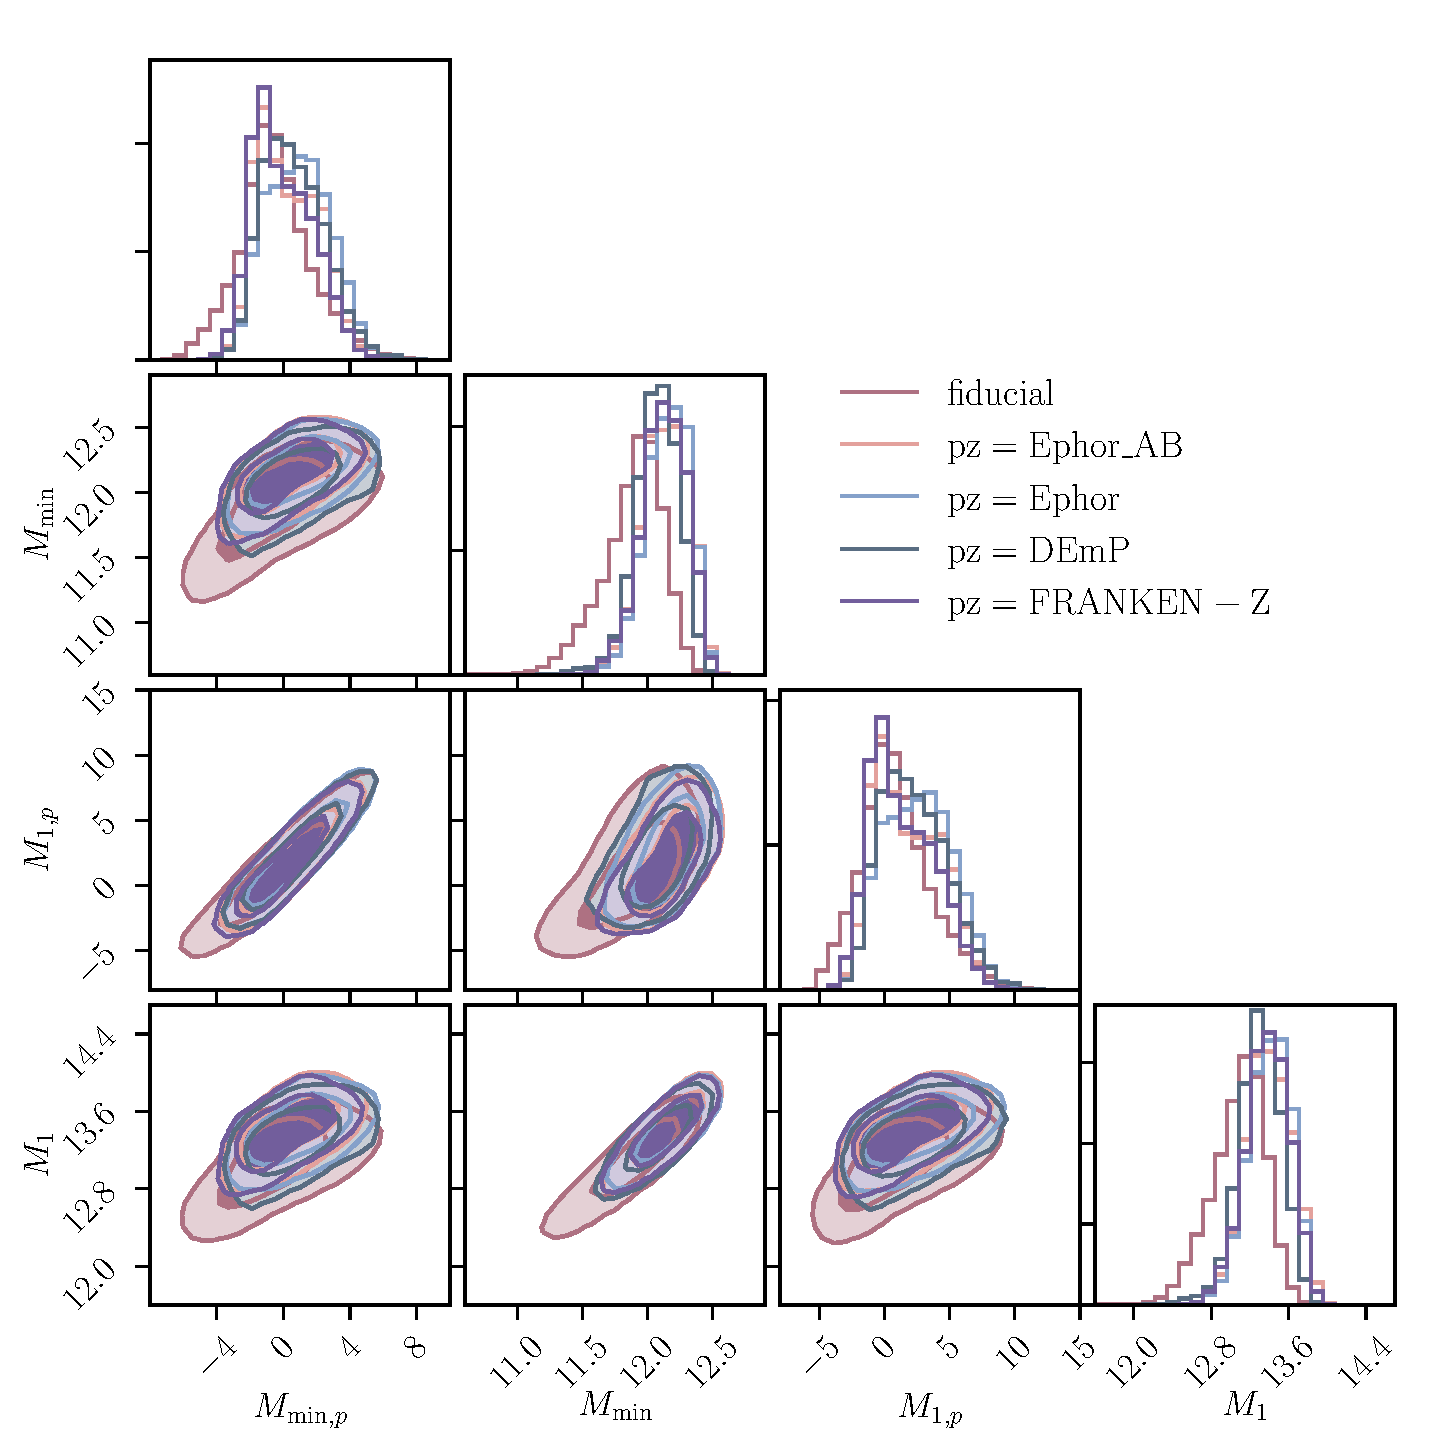
\includegraphics[width=0.95\textwidth]{figures/contours-Mmin-M1_mPk=HOD_fix=alpha-fc-sigmaM_HOD=zevol_fit=pz-shifts-pz-widths+prior=0p2_fit=auto+cross_cosmo=const_HOD-param=zfid_clfit=HOD-zevol_pz-methods.pdf}
\caption{Comparison of our fiducial HOD constraints to those obtained using the redshift distributions derived from \texttt{Ephor\_AB}, \texttt{Ephor}, \texttt{DEmP} and \texttt{FRANKEN-Z} marginalized over both shifts in the means and changes in the widths of the distributions. The inner (outer) contour shows the $68 \%$ c.l. ($95 \%$ c.l.).}
\label{fig:constraints-HOD-fit-pz-shifts+pz-widths-pz-methods}
\end{center}
\end{figure}
 
\begin{figure}
\begin{center}
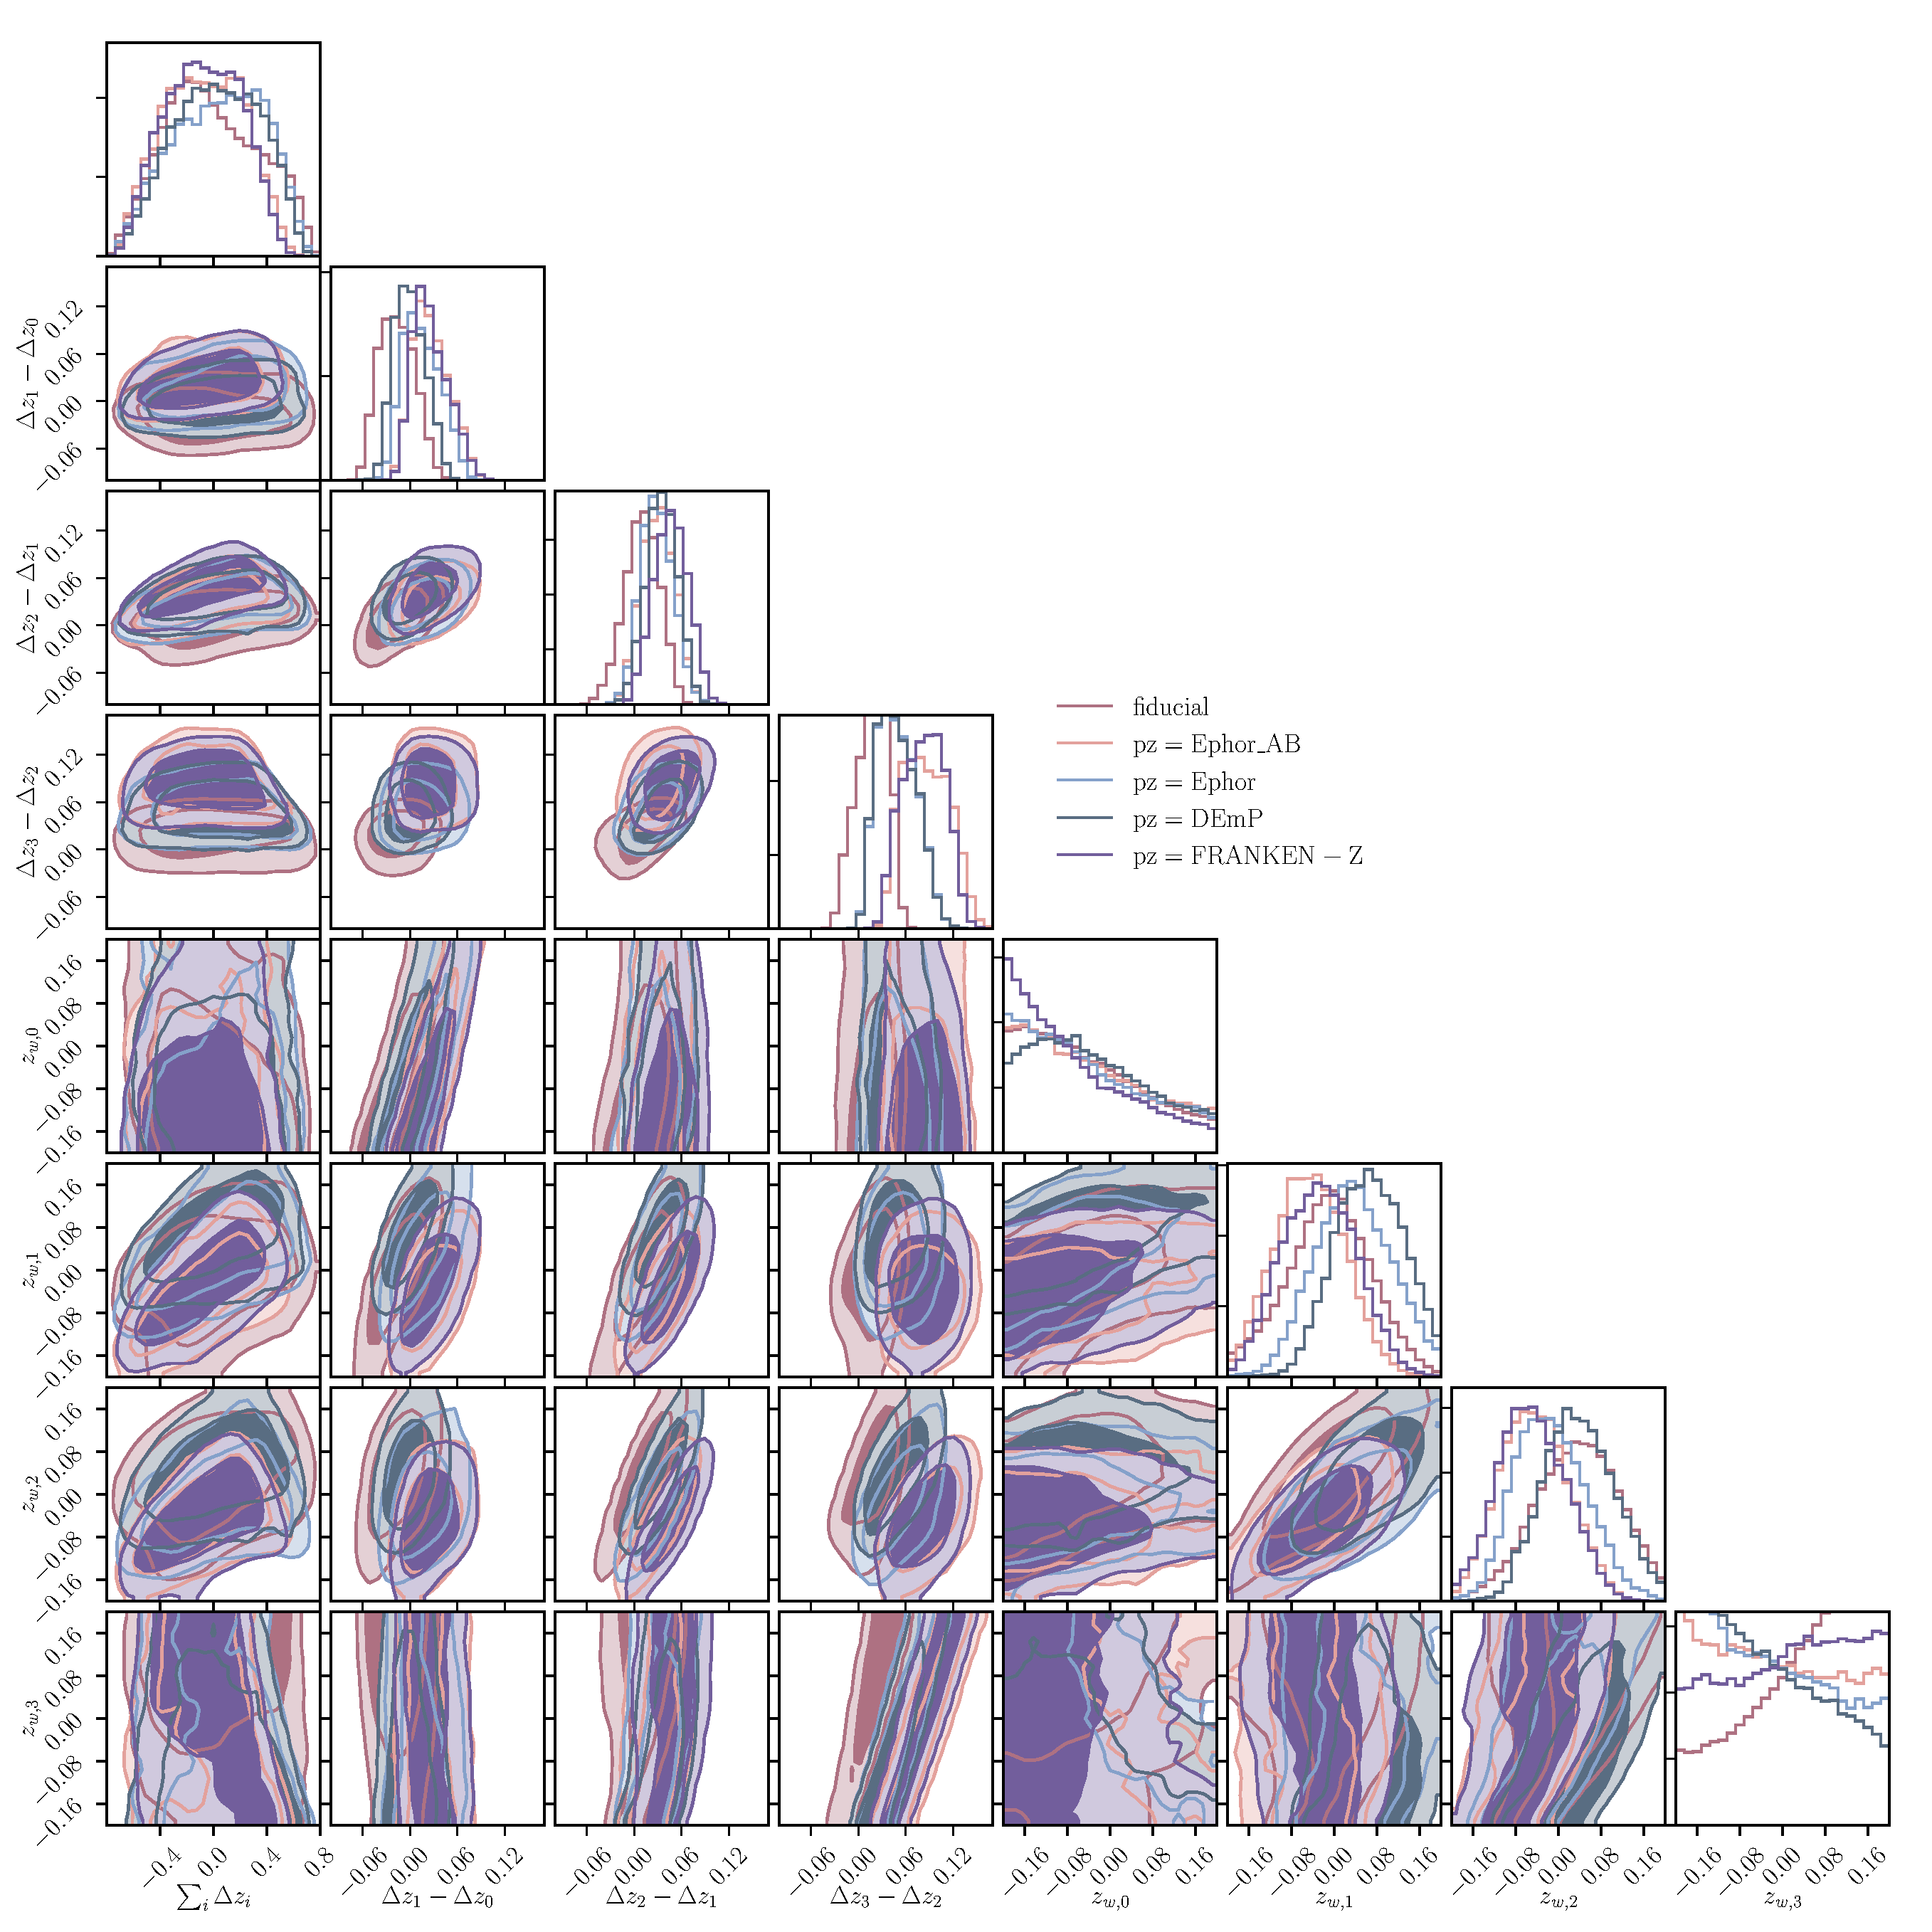
\includegraphics[width=0.95\textwidth]{figures/contours-pz-syst_mPk=HOD_fix=alpha-fc-sigmaM_HOD=zevol_fit=pz-shifts-pz-widths+prior=0p2_fit=auto+cross_cosmo=const_HOD-param=zfid_clfit=HOD-zevol_pz-methods.pdf}
\caption{Comparison of our fiducial constraints on photo-$z$ systematics parameters to those obtained using the redshift distributions derived from \texttt{Ephor\_AB}, \texttt{Ephor}, \texttt{DEmP} and \texttt{FRANKEN-Z}. The inner (outer) contour shows the $68 \%$ c.l. ($95 \%$ c.l.).}
\label{fig:constraints-pz-syst-fit-pz-shifts+pz-widths-pz-methods}
\end{center}
\end{figure}
 
\subsubsection{Interpretation of HOD results}\label{sssec:results.hod-constraints.constraints-interpretation}
As described in Sec.~\ref{sssec:results.hod-constraints.fiducial}, our best-fit HOD constraints predict both the minimal mass to host a central galaxy $M_{\mathrm{min}}(z)$ and the mass scale for satellites $M_{1}(z)$ to be redshift independent.
In order to understand this trend, it would be ideal to look at the rest-frame properties of the galaxies considered in our analysis and how these change with redshift. However, computing k-corrections and absolute magnitudes for broad-band photometric data can be challenging and we therefore choose an alternative approach. We cross-match galaxies passing our selection criteria within the HSC COSMOS field to galaxies also included in the COSMOS 30-band photometric catalog of \cite{2016ApJS..224...24L}. The COSMOS 30-band catalog contains, among others, absolute magnitudes in Subaru \texttt{B}-band, $M_{B}$, and Subaru \texttt{r+}-band, $M_{R}$. Using these quantities, we construct color-magnitude diagrams for all cross-matched galaxies. Fig.~\ref{fig:color-mag} shows the $M_{B}-M_{R}$ color as a function of $M_{R}$ magnitude for 10 equally spaced redshift bins in $z \in [0.15, 1.5]$\footnote{The galaxies are split into redshift bins according to COSMOS 30-band photometric redshifts. We note that we have repeated the analysis splitting the sample according to HSC \texttt{Ephor\_AB} photometric redshifts, finding consistent results.}. In this diagram, red galaxies populate the high $M_{B}-M_{R}$ color, high $M_{R}$ magnitude plane, while blue galaxies tend to have lower $M_{B}-M_{R}$ and $M_{R}$. As can be seen from the figure, red galaxies increasingly drop-out of the high redshift samples. We can quantify this effect by computing the fraction of red galaxies in our sample as a function of redshift: we empirically determine the separation between the blue and red clouds (denoted by the solid lines in the figure) and compute the fraction of galaxies in the red cloud as $f_{R} = \sfrac{N_{R}}{(N_{R}+N_{B})}$, where $N_{R}$ denotes the number of galaxies above the separation line, while $N_{B}$ is the number of galaxies below the line. Consistent with the figure, we find decreasing $f_{R}$ as a function of redshift. 

These results suggest that red galaxies are increasingly underrepresented with respect to blue galaxies in our sample at higher redshifts. This is probably due to the applied magnitude limit of $m_{\mathrm{lim}, i} < 24.5$, which translates to rest-frame wavelengths smaller than $4000$ \AA \, at redshifts $z \gtrsim 0.9$. As red galaxies become very faint at these wavelengths, they drop out of our selection, thus explaining the observed constancy of $M_{\mathrm{min}}(z)$ and $M_{1}(z)$ with redshift. This interpretation is consistent with the results from the HOD fits that predict a decreasing mean halo mass as a function of redshift for our sample (see Fig.~\ref{fig:HOD-redshift})

In Fig.~\ref{fig:HOD-redshift}, we additionally show the large-scale galaxy bias as a function of redshift derived from our best-fit HOD model. As can be seen, the large-scale bias scales approximately as $b(z) \sim \sfrac{1}{D(z)}$, where $D(z)$ denotes the linear growth factor. This behavior is consistent with e.g. studies of galaxies in the DEEP2 survey, which found constant clustering strengths as a function of redshift (and thus $b(z) \sim \sfrac{1}{D(z)}$) for magnitude-limited samples \cite{Coil:2004}. \todo{How about saying that a more thorough analysis of the color-dependence of clustering properties would be needed to fully characterize this effect and that we leave this for future work?}

\begin{figure}
\begin{center}
\subfigure{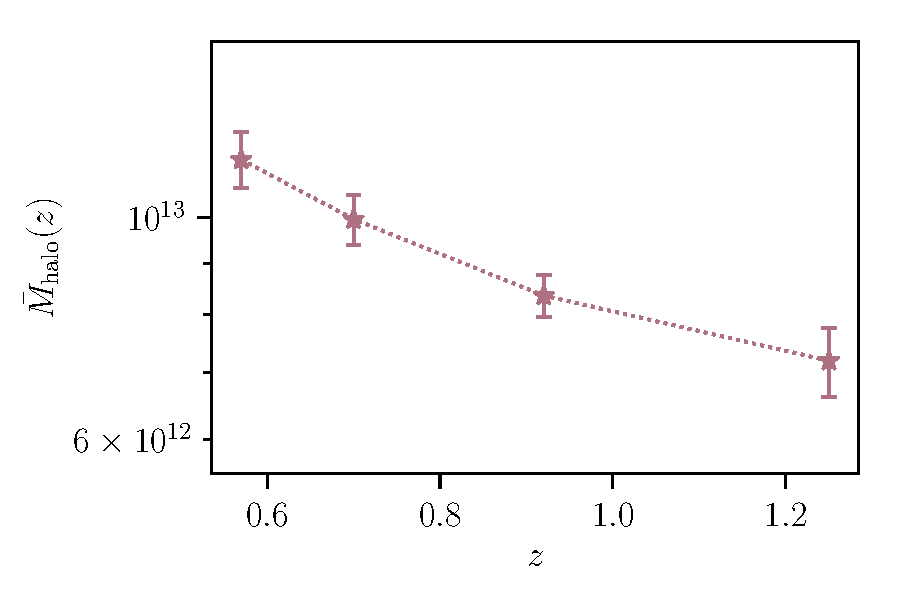
\includegraphics[width=0.32\textwidth]{figures/M_halo_mPk=HOD_fix=alpha-fc-sigmaM_HOD=zevol_fit=pz-shifts-pz-widths+prior=0p2_fit=auto+cross_cosmo=const_cov=G+NG+SSC-LINBIAS_HOD-param=zfid_clfit=HOD-zevol.pdf}} 
\subfigure{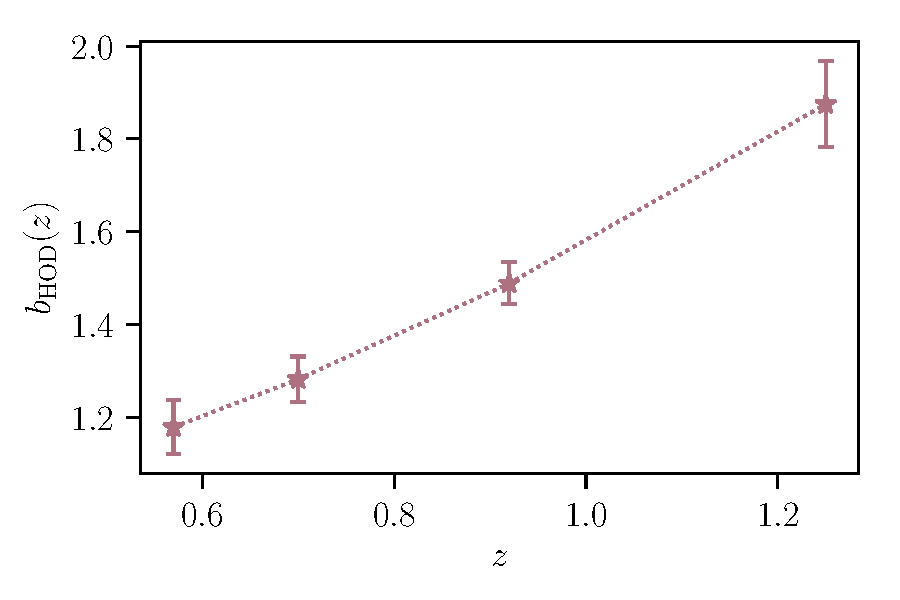
\includegraphics[width=0.32\textwidth]{figures/bias-redshift_mPk=HOD_fix=alpha-fc-sigmaM_HOD=zevol_fit=pz-shifts-pz-widths+prior=0p2_fit=auto+cross_cosmo=const_cov=G+NG+SSC-LINBIAS_HOD-param=zfid_clfit=HOD-zevol.pdf}}
\subfigure{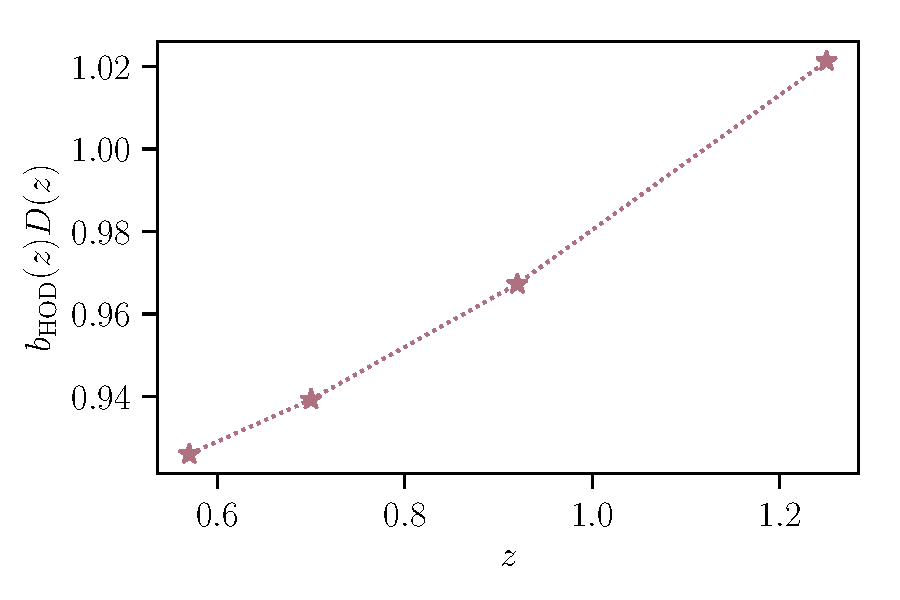
\includegraphics[width=0.32\textwidth]{figures/bias-growth_mPk=HOD_fix=alpha-fc-sigmaM_HOD=zevol_fit=pz-shifts-pz-widths+prior=0p2_fit=auto+cross_cosmo=const_cov=G+NG+SSC-LINBIAS_HOD-param=zfid_clfit=HOD-zevol.pdf}} 
\caption{Redshift dependence of the mean halo mass $\bar{M}_{\mathrm{halo}}$ and the large-scale galaxy bias $b_{\mathrm{HOD}}$ as derived from our best-fit HOD model. The third panel illustrates the empirical scaling $b(z) \sim \sfrac{1}{D(z)}$ derived from the galaxy sample used in this analysis.}
\label{fig:HOD-redshift}
\end{center}
\end{figure}

%\begin{figure}
%\begin{center}
%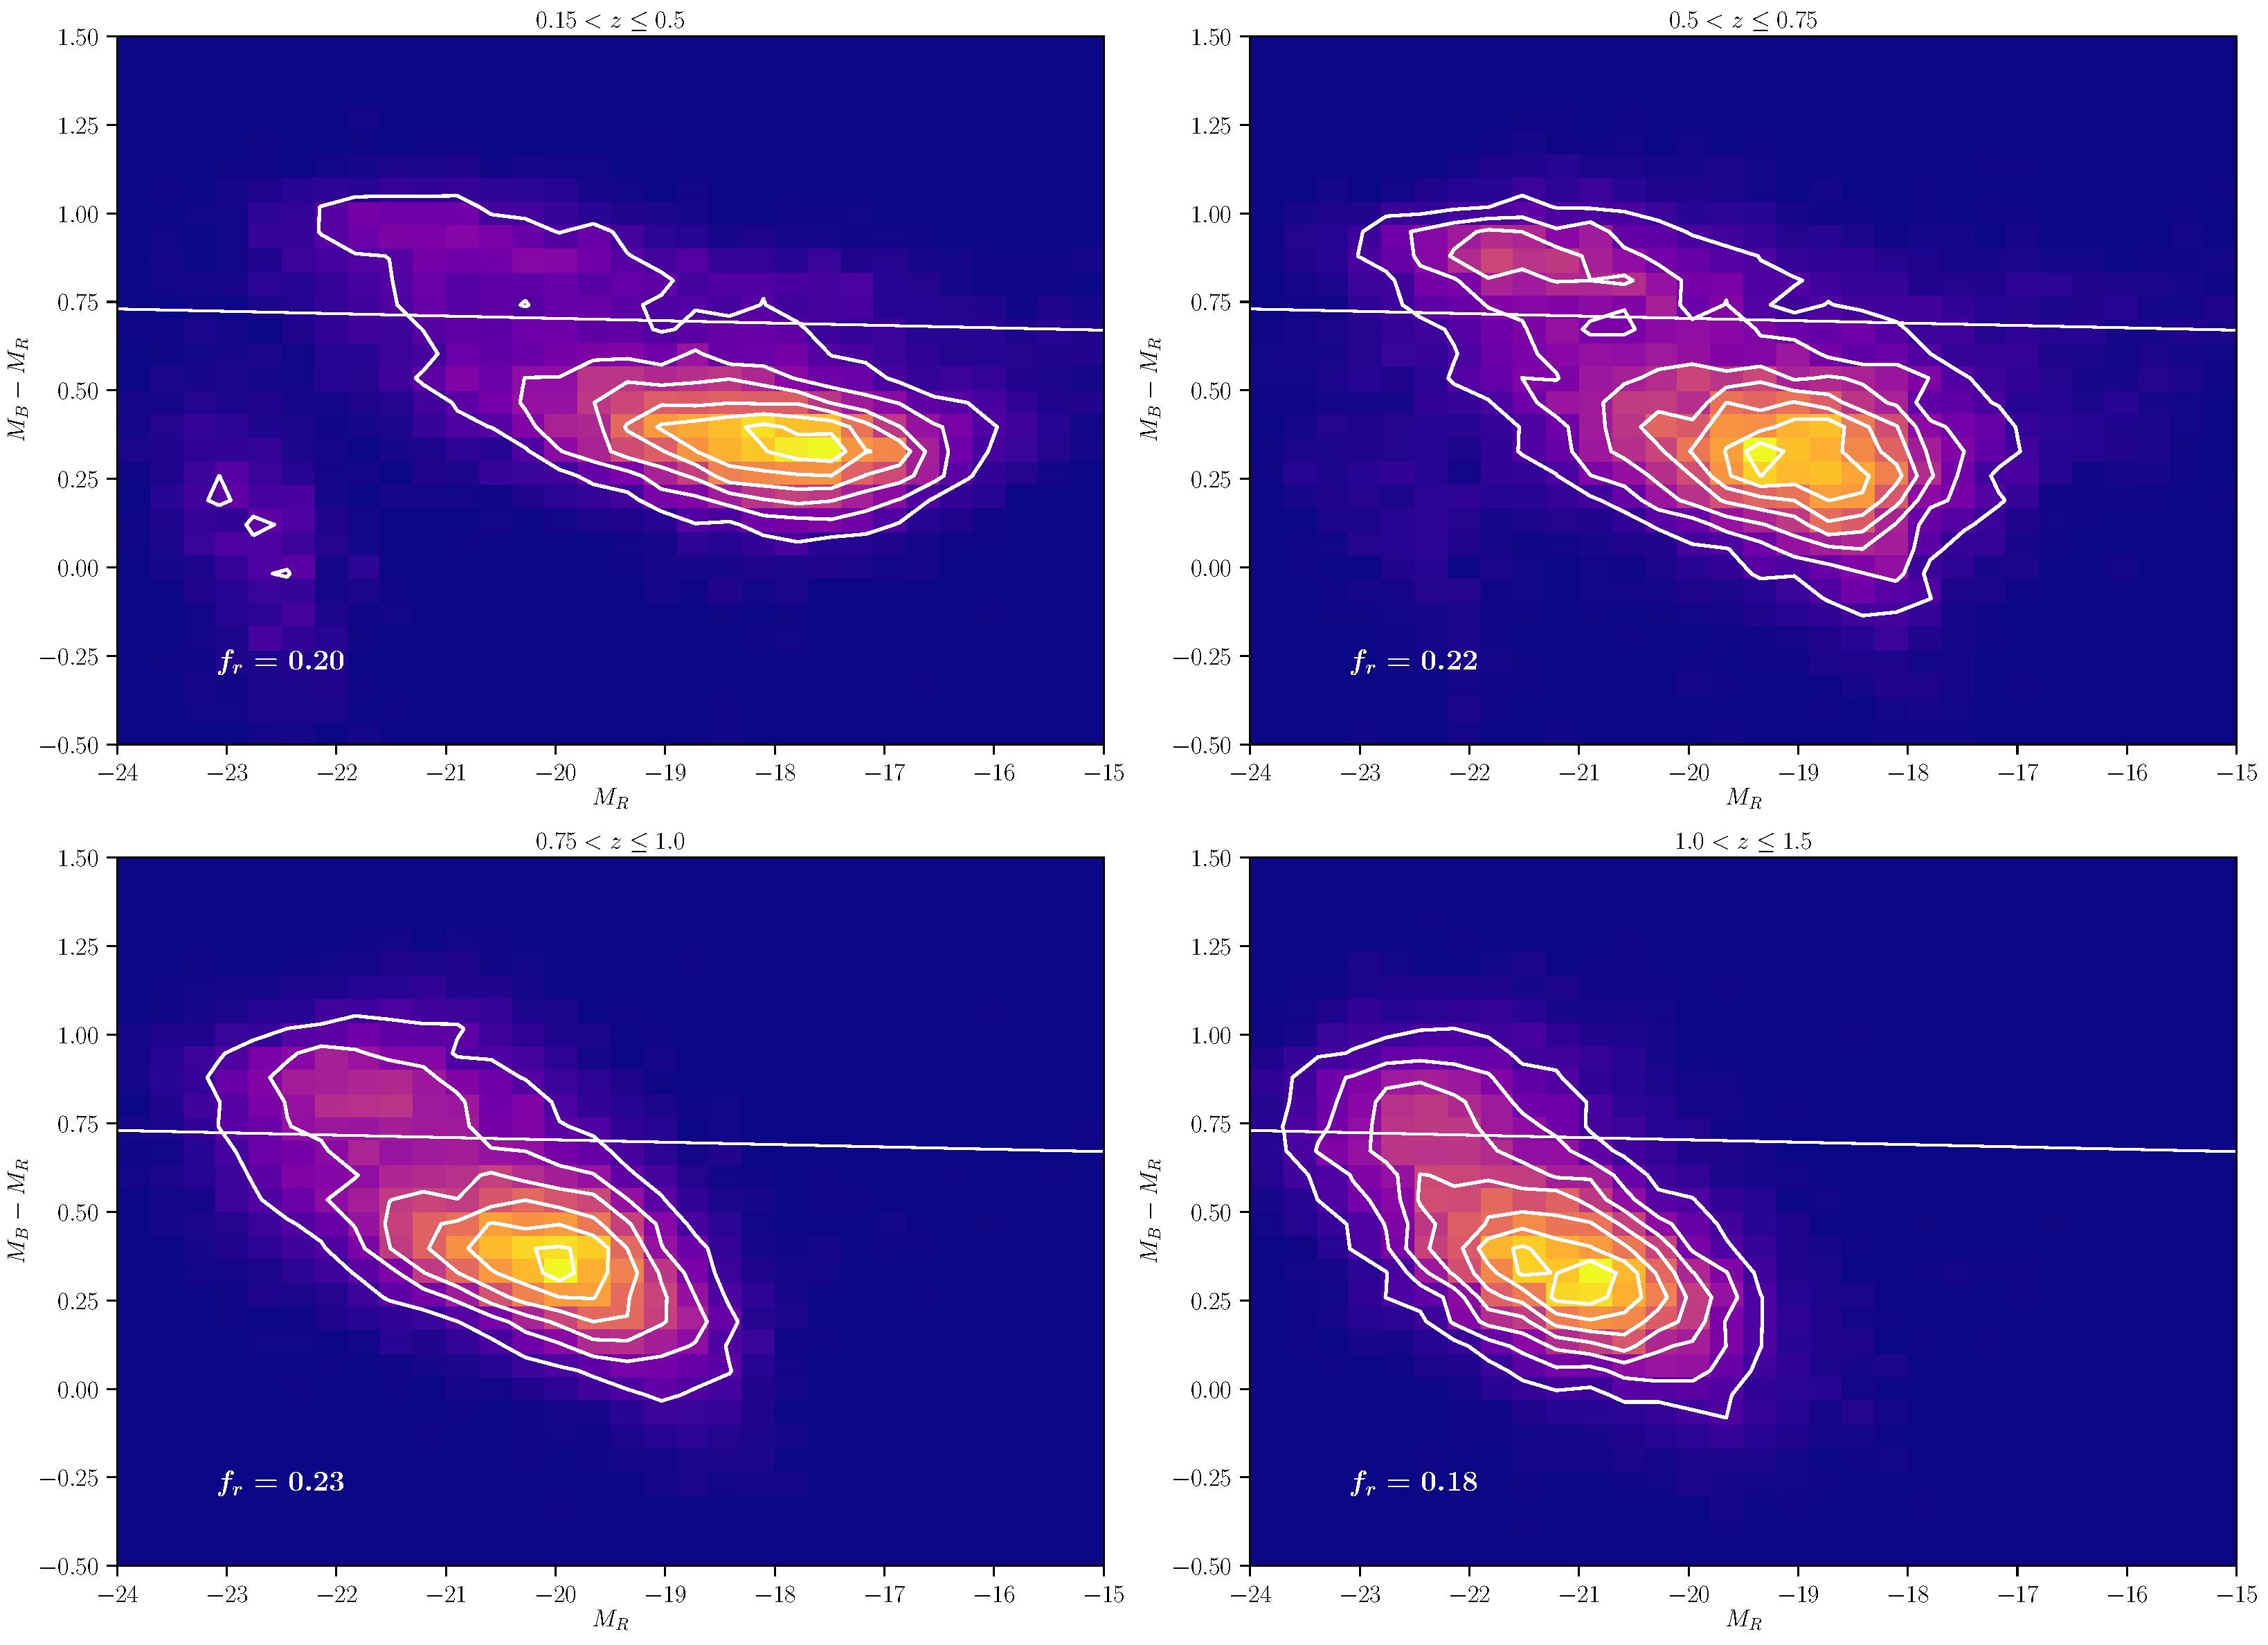
\includegraphics[scale=0.55]{figures/color-magnitude_cut=pz_best_eab_nbin=4_weights=True.pdf}
%\caption{Synopsis of the framework for integrated probe combination employed in this work.}
%\label{fig:color-mag}
%\end{center}
%\end{figure}

      \begin{sidewaysfigure}
        \begin{center}
          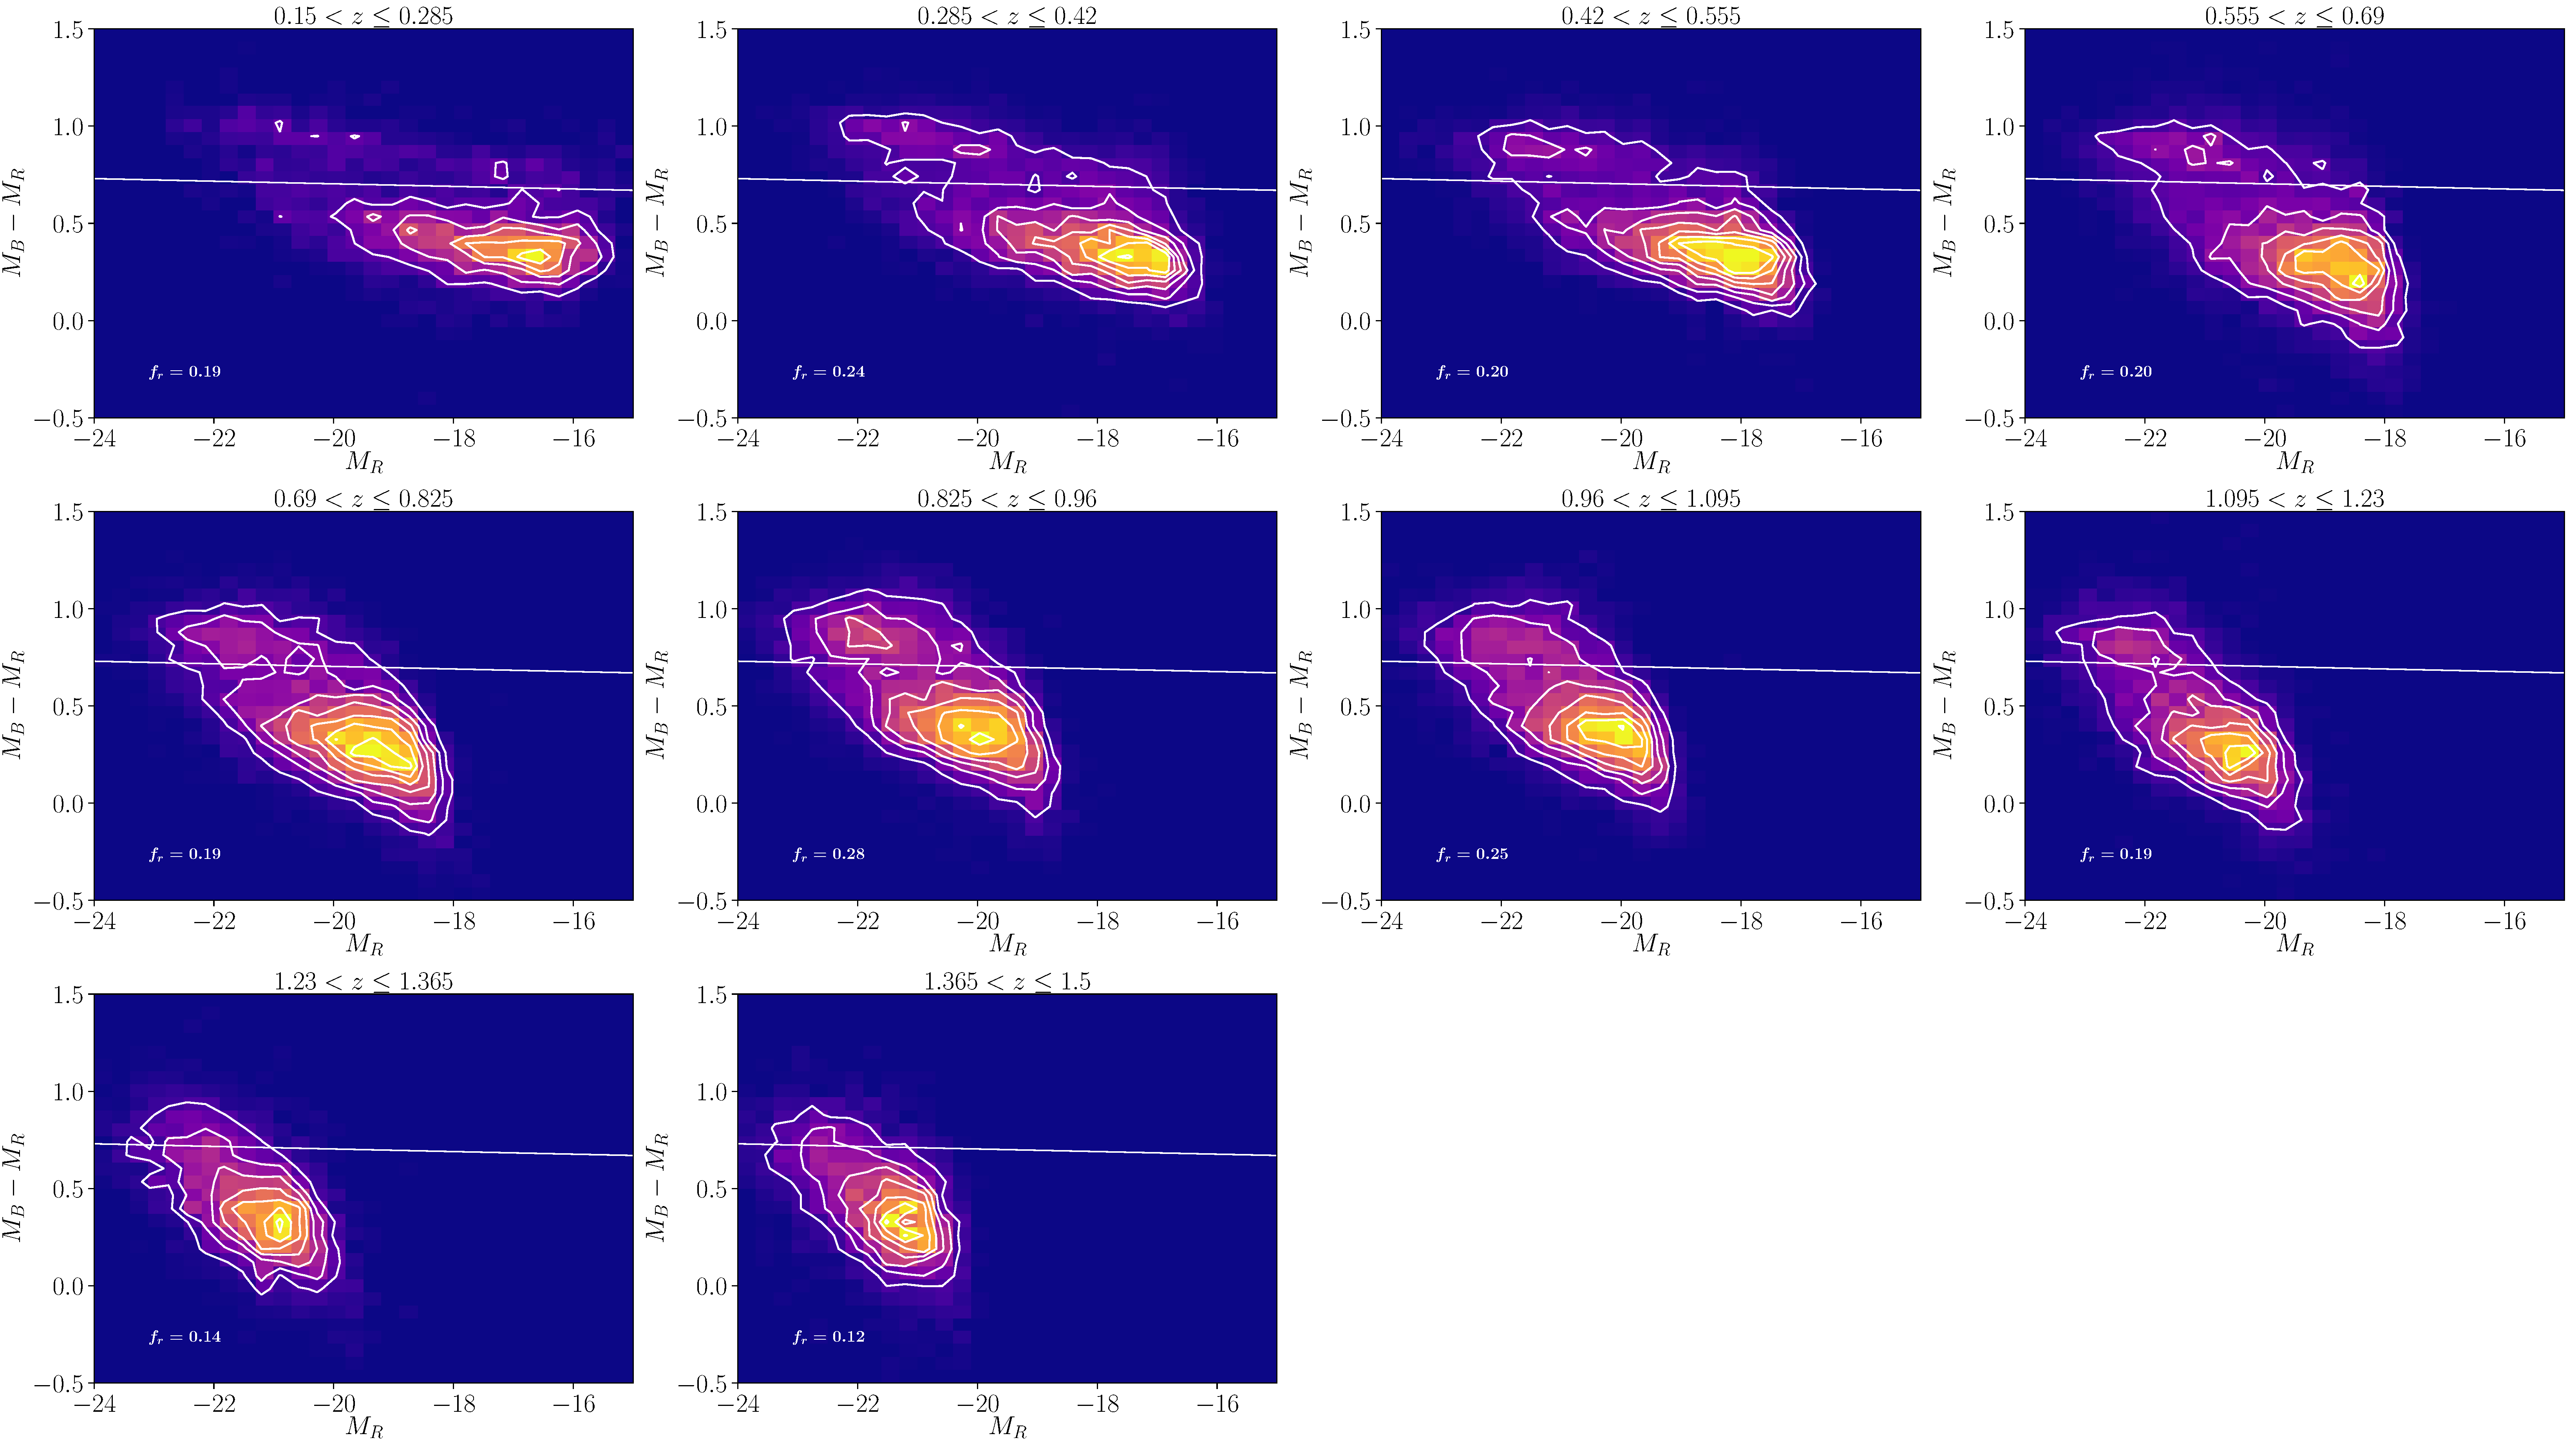
\includegraphics[width=0.95\textwidth]{figures/color-magnitude_cut=COSMOS30_nbin=10_weights=True.pdf}
          \caption{Color-magnitude diagrams of COSMOS 30-band galaxies cross-matched to HSC galaxies passing our selection cuts for 10 tomographic redshift bins with $z \in [0.15, 1.5]$.}
          \label{fig:color-mag}
        \end{center}
      \end{sidewaysfigure}
      
 \subsection{Magnification}\label{ssec:results.magnification}

    In addition to intrinsic correlations between galaxy positions, there exist several additional effects affecting the observed clustering of galaxies. One of these is the magnification of distant sources due to gravitational lensing by the intervening LSS, an effect usually called magnification bias (e.g. \cite{Schneider:1989, Narayan:1989}). The main effect of magnification on the statistical distribution of galaxies is to increase observed galaxy fluxes, thus allowing dim galaxies to pass survey selection thresholds, and to alter their observed angular positions. The combined effect, is a position-dependent modulation of the number density that distorts the clustering pattern. It has been shown that the clustering signal due to magnification can be comparable to the intrinsic clustering signal for cross-correlations between widely separated redshift bins (see e.g. \cite{Challinor:2011}).

    In the presence of magnification, the equations in Section \ref{ssec:methods.theory} get slightly modified. The projected galaxy overdensity becomes:
    \begin{equation}
      \delta^i_g(\nv)=\int \mathrm{d}z\,\left[p^i(z)\,\Delta_g+\frac{W_\mu^i(z)}{H(z)}\nabla_\theta^2\nabla^{-2}\Delta_m\right],
    \end{equation}
    where $\Delta_m$ is the 3D matter overdensity (we have omitted the dependence on $t$ and $\chi\nv$ for brevity) and $W_\mu$ is the magnification kernel
    \begin{equation}
      W_\mu(z)=\frac{3H_0^2\Omega_M(1+z)}{2}\int_z^\infty \mathrm{d}z'\,p^i(z)\,\left(5s(z')-2\right)\,\frac{\chi(z')-\chi(z)}{\chi(z)\chi(z')}.
    \end{equation}
    Here, $H_0\equiv H(z=0)$, $\Omega_M$ is the cosmological matter fraction, and $s$ is the logarithmic slope of the cumulative apparent magnitude distribution $N(<m, z)$:
    \begin{equation}
      s(z) \equiv \frac{\partial \log_{10}N(<m, z)}{\partial m},
      \label{eq:s-func}
    \end{equation}
    where $m$ denotes the observed magnitude.
    The angular power spectrum is then given by:
    \begin{equation}\label{eq:cell_gg_wmag}
      C^{ij}_\ell = \int \mathrm{d}z\,\frac{H(z)}{\chi^2(z)}\left[p^ip^j\,P_{gg}+\left(p^iW_\mu^j+p^jW_\mu^i\right)\frac{\ell(\ell+1)}{Hk^2}P_{gm}+W_\mu^iW_\mu^j\left(\frac{\ell(\ell+1)}{Hk^2}\right)^2P_{mm}\right],
    \end{equation}
    where $P_{mm}$ is the 3D power spectrum of matter fluctuations, $P_{gm}$ is the galaxy-matter cross-spectrum and we have omitted the dependence of all quantities on $z$ or $k=(\ell+1/2)/\chi$ for brevity.

    The magnitude of the magnification signal crucially depends on the derivative of the galaxy number counts with respect to observed magnitude, $s(z)$. In order to obtain a data-driven model for magnification in our particular sample, we therefore estimate $s(z)$ from the observed number counts. Using linear least squares, we fit a fourth-order polynomial to the logarithm of the observed cumulative apparent $\tt{i}$-band magnitude distribution $N(<m, z)$ in each of the four tomographic redshift bins considered in our analysis. We then determine $s(z)$ at the effective redshift of each bin\footnote{We define the effective redshift for each tomographic bin as the mean redshift of the galaxy distribution.} by taking the derivative of the best-fit function at the magnitude limit of our sample, i.e. $m_{i, \mathrm{lim}} = 24.5$. In addition to the WIDE HSC galaxy data used in this work, PDR1 also contains data from two deep patches, called DEEP and UDEEP. We repeat the above analysis with these galaxy samples to ensure the stability of our results. As an example, Fig.~\ref{fig:s-func-estimation} shows the observed number counts as a function of $i$-band magnitude for the lowest redshift bin in the WIDE sample alongside the derived best-fit function. In Fig.~\ref{fig:s-func-estimation}, we show the $s(z)$ functions derived as outlined above for HSC WIDE, DEEP and UDEEP. As can be seen, the three estimates agree well with each other and we use the $s(z)$ function derived from our fiducial WIDE sample in the following.
    \begin{figure}
      \begin{center}
        \subfigure[Cumulative galaxy number counts as a function of $i$-band magnitude for lowest tomographic redshift bin.]{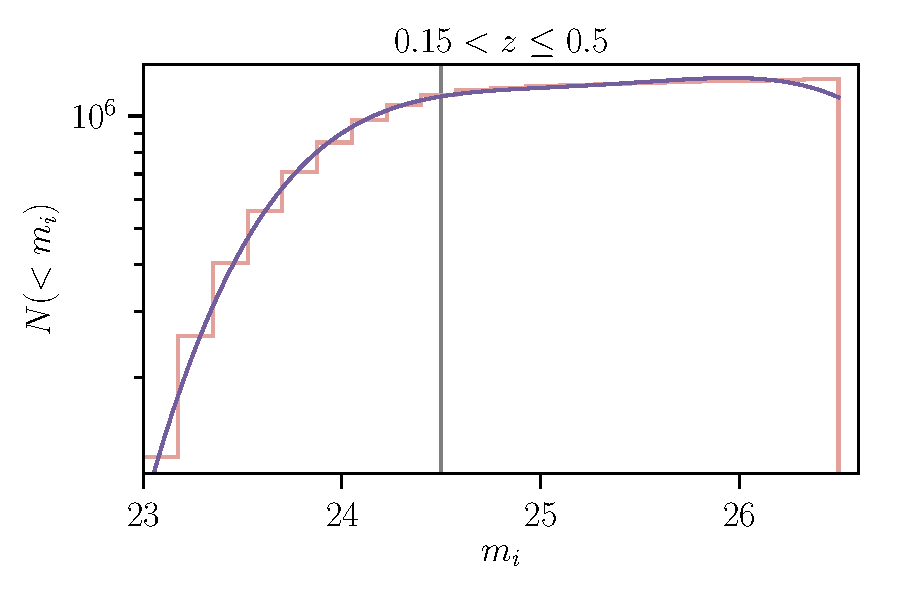
\includegraphics[width=0.49\textwidth]{figures/mag-dist-cumulative=True+fit-mmin=23-sample=WIDE-bin=0.pdf}}
        \subfigure[Comparison of $s(z)$ (see Eq.~\ref{eq:s-func}) derived using WIDE, DEEP and UDEEP HSC galaxy samples.]{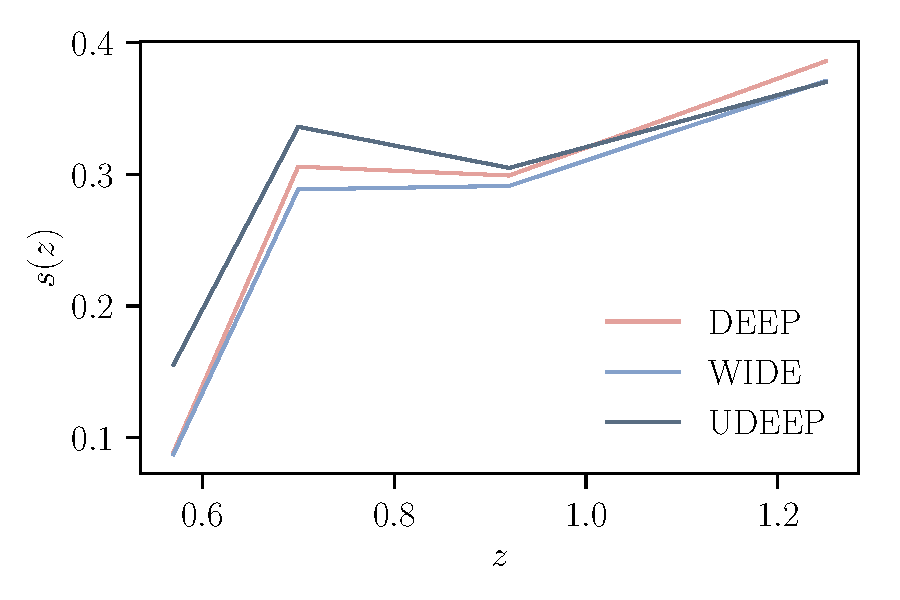
\includegraphics[width=0.49\textwidth]{figures/s-z-func-samples=WIDE-DEEP-UDEEP.pdf}} 
        \caption{Illustration of data-driven estimation of $s(z)$ for galaxy sample used in our analysis.} 
        \label{fig:s-func-estimation}
      \end{center}
    \end{figure}

    Using the estimated $s(z)$, we can derive theoretical predictions for the angular galaxy power spectra in presence of magnification. In order to investigate the sensitivity of the data to magnification we run two different MCMC analyses: in the first case, we fix the magnification amplitude to the predictions from the empirically determined $s(z)$ function. In the second case we include an additional magnification parameter $A_{\mu}$ that scales the amplitude of the magnification kernel $W_{\mu}$ and we fit it alongside our fiducial parameter set.

    From a joint fit to all auto- and cross power spectra we obtain $A_{\mu} = 2.18 \pm 0.74$ and the constraint is shown in Fig.~\ref{fig:constraints-fit=mag-bias-ampl_fit=auto+cross-vs-fit=mag-bias-ampl_fit=auto}. This constitutes a $\sim 2.9 \sigma$ detection of magnification from our HSC sample. Furthermore, this constraint is consistent with our fiducial model for $s(z)$, which corresponds to $A_{\mu} = 1$, at the $\sim 1.6 \sigma$ level. This marginal inconsistency is probably due to uncertainties in the data-driven estimation of $s(z)$. The best-fit $\chi^{2}$ including magnification is $\chi^{2} = 69.0$\footnote{This is consistent with the case in which we set $A_{\mu}=1$, where we obtain consistent constraints with best-fit $\chi^{2} = 72.8$, as can be seen from Tab.~\ref{tab:constraints_robustness}.}, which, computing the degrees of freedom as $\nu = N_{\mathrm{data}} - N_{\mathrm{param}} = 94 - 15 = 79$, leads to $\chi^{2}_{\mathrm{red}} = \sfrac{\chi^{2}}{\nu} = 0.87$ ($p$-value $= 0.78$). This corresponds to an improvement in $\chi^{2}$ compared to the fiducial analysis of $\Delta \chi^{2} = 86.2 - 69.0 = 17.2$, consistent with the $\sim 3 \sigma$ detection. Fig.~\ref{fig:cls-best-fit} shows the corresponding theoretical predictions derived from the maximum likelihood parameters alongside the observed data. The constraints on HOD parameters obtained when including magnification agree very well with our fiducial constraints, as can be seen from Fig.~\ref{fig:constraints-no-mag-bias-vs-fit=mag-bias-ampl}. In addition, we find the significance of the magnification detection to be largely insensitive to photo-$z$ systematics modeling choices, as it is not significantly affected by relaxing our photo-$z$ systematics model by fixing $z_{w, i} = 0$. 

    In order to identify the part of the data vector driving the constraints on $A_{\mu}$, we repeat this analysis only including the auto power spectra. The comparison between the constraints on $A_{\mu}$ from auto- and cross power spectra to those obtained from auto power spectra alone in shown in Fig.~\ref{fig:constraints-fit=mag-bias-ampl_fit=auto+cross-vs-fit=mag-bias-ampl_fit=auto}. As can be seen, the auto power spectra alone do not constrain $A_{\mu}$, which implies that the constraints on the magnification amplitude are solely driven by the cross power spectra. This sensitivity of the cross power spectra to magnification mainly stems from the fact that the intrinsic cross correlations between widely separated bins are small, which leads to an increased sensitivity to any non-intrinsic source of cross correlation, such as magnification. In analogy to the results for the photo-$z$ systematics parameters, we thus find that cross power spectra carry important information and it will thus be beneficial to include these cross correlations in current and future photometric clustering analyses. 

    \begin{figure}
      \begin{center}
        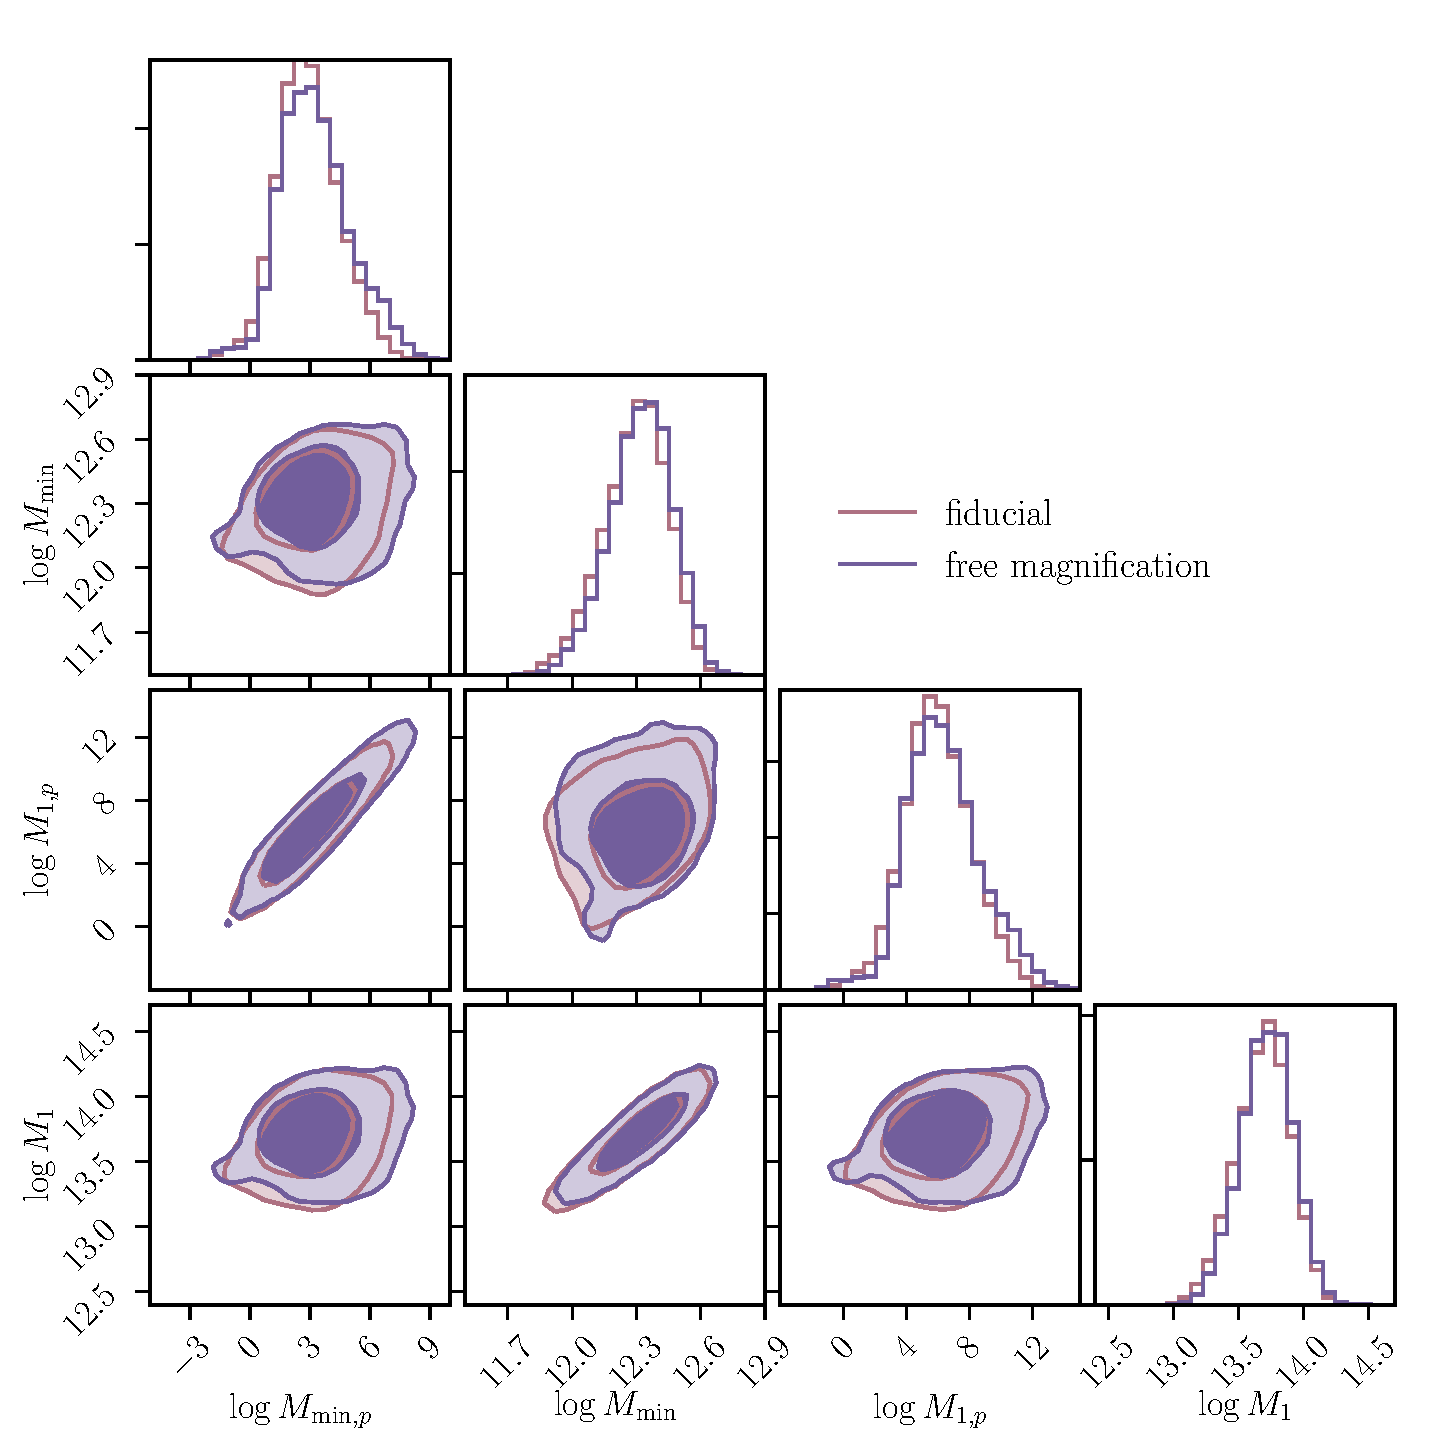
\includegraphics[width=0.95\textwidth]{figures/contours-Mmin-M1_mPk=HOD_fix=alpha-fc-sigmaM_HOD=zevol_fit=pz-shifts+prior=0p2-pz-widths+prior=0p2_fit=auto+cross_cosmo=const-LINBIAS_HOD-param=zfid_clfit=HOD-zevol_no-mag-bias-vs-mag-bias-free.pdf}
        \caption{Comparison of our fiducial HOD constraints to those obtained when varying the magnification amplitude. The inner (outer) contour shows the $68 \%$ c.l. ($95 \%$ c.l.).}
        \label{fig:constraints-no-mag-bias-vs-fit=mag-bias-ampl}
      \end{center}
    \end{figure}

    \begin{figure}
      \begin{center}
        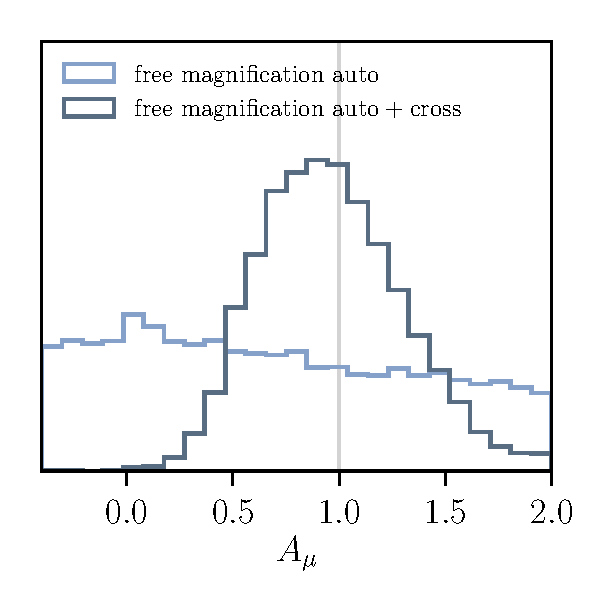
\includegraphics[width=0.3\textwidth]{figures/contours-A_mu_mPk=HOD_fix=alpha-fc-sigmaM_HOD=zevol_fit=pz-shifts+prior=0p2-pz-widths+prior=0p2_fit=auto+cross_cosmo=const-LINBIAS_HOD-param=zfid_clfit=HOD-zevol_mag-bias-free-fit=auto+cross-vs-mag-bias-free-fit=auto.pdf}
        \caption{Comparison of the constraints on magnification amplitude obtained from auto power spectra alone to those obtained from auto and cross power spectra. The solid line denotes the expectation value of the magnification amplitude determined from our data-driven fiducial model described in Sec.~\ref{ssec:results.magnification}.}
        \label{fig:constraints-fit=mag-bias-ampl_fit=auto+cross-vs-fit=mag-bias-ampl_fit=auto}
      \end{center}
    \end{figure}

  \subsection{Joint cosmology and HOD constraints}\label{ssec:results.cosmo}
    Additionally we also consider jointly fitting cosmological, HOD and photo-$z$ systematics parameters. This analysis should be regarded as exploratory and only provide a means to illustrate the potential of photometric galaxy clustering analyses to jointly constrain these parameters. An in-depth cosmological analysis would require validation of the analysis and HOD modeling framework on simulations, which is beyond the scope of this work.

    To illustrate the cosmological constraining power of the data considered in our analysis, we allow for variations in the r.m.s. of linear matter fluctuations in spheres of comoving radius 8 $h^{-1}$ Mpc, $\sigma_{8}$, and the fractional cold matter density today, $\Omega_{c}$, in addition to our baseline set of parameters (c.f. Sec.~\ref{ssec:methods.constr}). All other cosmological parameters remain fixed to their fiducial Planck 2018 values. From a joint fit to all auto- and cross power spectra we obtain $\sigma_{8} = 0.807\substack{+0.149 \\ -0.143}$ and $\Omega_{c} = 0.237 \pm 0.025$, consistent with our assumed fiducial cosmology. The corresponding constraints are shown in Fig.~\ref{fig:constraints-fit=Oc+s8}. As can be seen from Tab.~\ref{tab:constraints_robustness}, the derived constraints on HOD parameters agree well with our fiducial results, which shows that our HOD constraints are robust to variations in $\Omega_{c}$ and $\sigma_{8}$ as allowed by the data. This exploratory cosmological analysis further shows that the data are able to constrain $\Omega_{c}$ while $\sigma_{8}$ is largely unconstrained, showing that the halo model is sufficiently flexible to allow effective marginalization over linear galaxy bias. Therefore, photometric current and future galaxy clustering analyses constitute a promising way to jointly constrain HOD and cosmological parameters, which we leave to future work. 
 
    \begin{figure}
      \begin{center}
        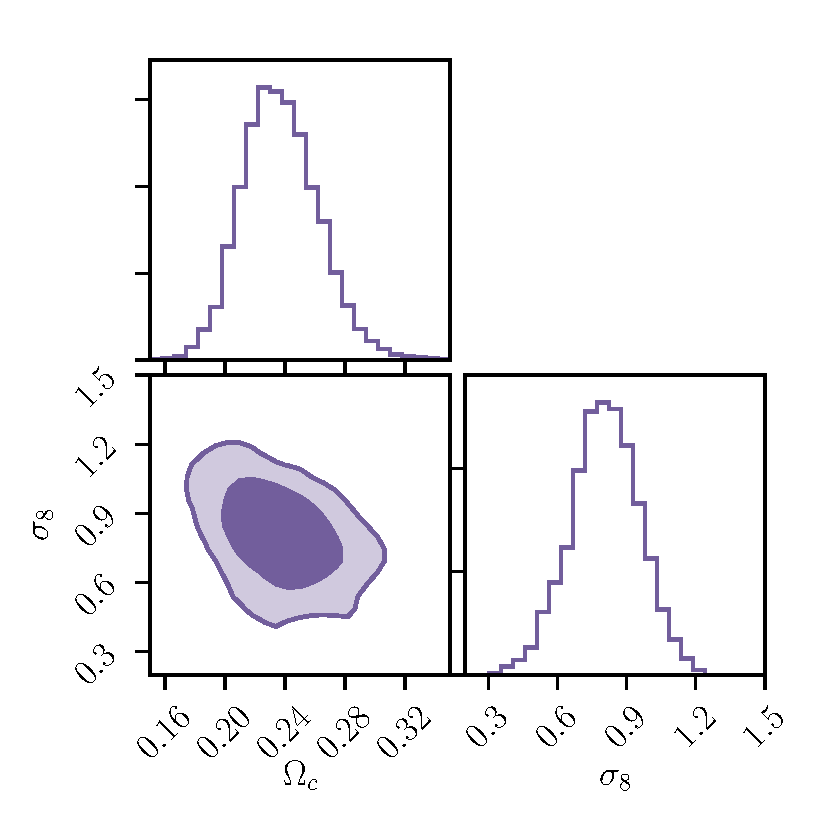
\includegraphics[width=0.49\textwidth]{figures/contours-Oc-s8_mPk=HOD_fix=alpha-fc-sigmaM_HOD=zevol_fit=pz-shifts+prior=0p2-pz-widths+prior=0p2_fit=auto+cross_cosmo=const-LINBIAS_HOD-param=zfid_clfit=HOD-zevol_fit=Oc+s8.pdf}
        \caption{Constraints on cosmological parameters obtained from a joint fit to all auto- and cross power spectra. The inner (outer) contour shows the $68 \%$ c.l. ($95 \%$ c.l.).}
        \label{fig:constraints-fit=Oc+s8}
      \end{center}
    \end{figure} 
    
\subsection{Constraints on linear galaxy bias for different magnitude-limited samples}\label{ssec:results.mag_cuts}

Finally we use our analysis pipeline described in Sec.~\ref{sec:methods} to investigate the dependence of galaxy clustering on limiting magnitude $m_{\mathrm{lim}}$ of the sample and derive an approximate fitting function for the linear galaxy bias as a function of redshift and $m_{\mathrm{lim}}$. 

To this end we split our fiducial galaxy sample into four brighter subsamples with limiting magnitudes $i_{\mathrm{corr}} < 20.5$, $i_{\mathrm{corr}} < 21.5$, $i_{\mathrm{corr}} < 22.5$ and $i_{\mathrm{corr}} < 23.5$, respectively. We then subdivide each of these samples into four redshift bins of approximately equal galaxy number and use our pipeline to compute constraints on HOD parameters for our fiducial analysis variant. This allows us to derive constraints on the large-scale galaxy bias as a function of redshift for each sample. We determine the bias from the mean of the posterior distribution as we find it to yield more stable constraints than the best-fit value. The results for the bias evaluated at the effective redshift of each tomographic bin are shown in Fig.~\ref{fig:magnitude-cuts-bias}, alongside the results for our fiducial sample. As can be seen, we find the linear bias to increase for decreasing limiting magnitude, as expected. Furthermore, the redshift-dependence of the bias can be roughly approximated as inversely proportional to the growth factor, $b(z) \sim \sfrac{1}{D(z)}$, for all samples. In order to obtain a fitting function for the large-scale galaxy bias as a function of redshift and limiting magnitude, we assume it to be separable in $z$ and $m_{\mathrm{lim}}$ and make the following Ansatz:
\begin{equation}
b(z, m_{\mathrm{lim}}) = \bar{b}(m_{\mathrm{lim}}) D(z)^{\alpha}.
\label{eq:bias-fit-func}
\end{equation}  
We determine the values of $\alpha$ and $\bar{b}(m_{\mathrm{lim}})$ in a two-step weighted, linear least squares fit: we first fit Eq.~\ref{eq:bias-fit-func} to all five samples separately and determine our fiducial $\alpha$ as the median of these values\footnote{We note that we find slightly better results using the median, which is the reason for preferring it over the mean.}. We then fit Eq.~\ref{eq:bias-fit-func} to all samples again, obtaining constraints on $\bar{b}(m_{\mathrm{lim}})$ for $\alpha$ fixed to our fiducial value. In a last step, we fit a linear function to $\bar{b}(m_{\mathrm{lim}})$, finally yielding
\begin{align}
\alpha &= -1.32, \\
\bar{b}(m_{\mathrm{lim}}) &= b_{1}m_{\mathrm{lim}} + b_{0},
\label{eq:bias-fit-func}
\end{align}  
where $b_{1} = -0.0627$ and $b_{0} = 2.35$. The results from this fitting function are shown as solid lines in Fig.~\ref{fig:magnitude-cuts-bias}, alongside the values obtained from the HOD fit. As can be seen, the fitting function provides a rather good fit and it might thus become a useful tool for e.g. modeling the galaxy bias when forecasting the constraining power of magnitude-limited galaxy samples.

\begin{figure}
\begin{center}
\subfigure{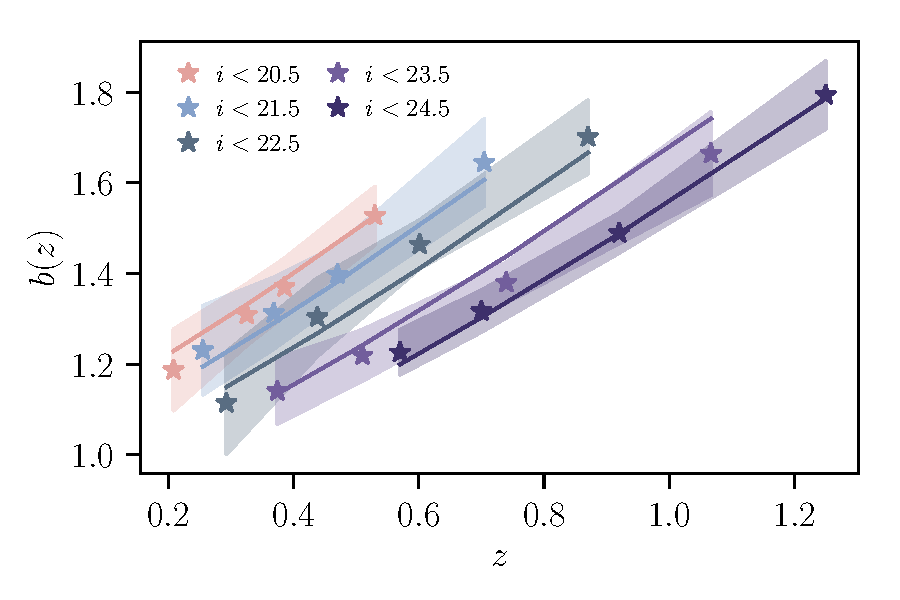
\includegraphics[width=0.32\textwidth]{figures/bias-redshift_mPk=HOD_fix=alpha-fc-sigmaM_HOD=zevol_fit=pz-shifts-pz-widths+prior=0p2_fit=auto+cross_cosmo=const_cov=G+NG+SSC-LINBIAS_HOD-param=zfid_clfit=HOD-zevol_magnitude_cuts_fitting-func.pdf}} 
\subfigure{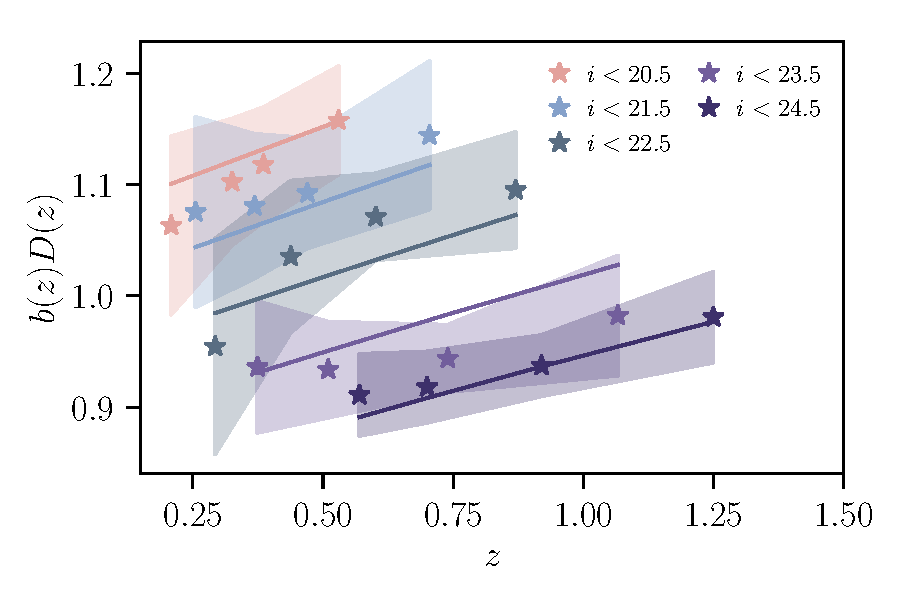
\includegraphics[width=0.32\textwidth]{figures/bias-growth-redshift_mPk=HOD_fix=alpha-fc-sigmaM_HOD=zevol_fit=pz-shifts-pz-widths+prior=0p2_fit=auto+cross_cosmo=const_cov=G+NG+SSC-LINBIAS_HOD-param=zfid_clfit=HOD-zevol_magnitude_cuts_fitting-func.pdf}}
\subfigure{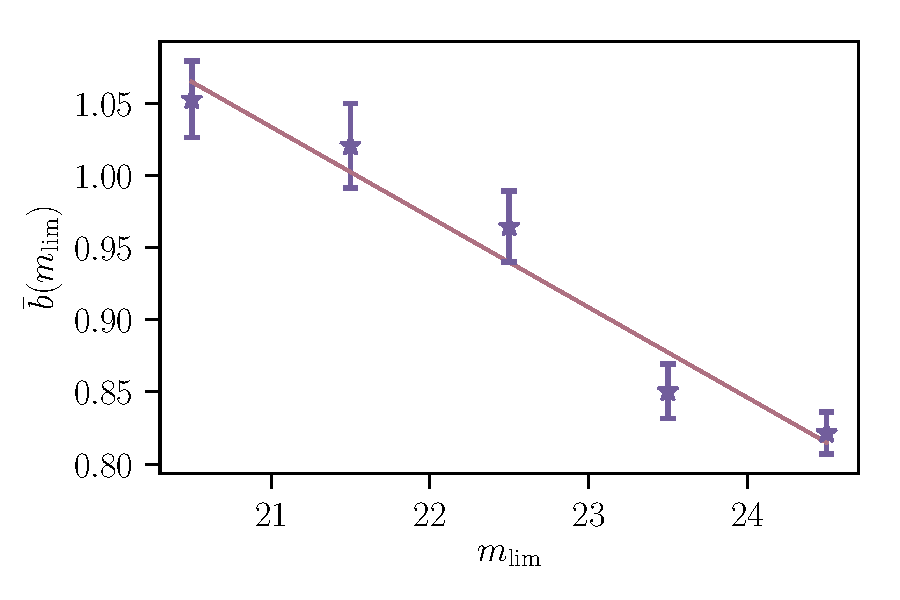
\includegraphics[width=0.32\textwidth]{figures/bias-mlim_mPk=HOD_fix=alpha-fc-sigmaM_HOD=zevol_fit=pz-shifts-pz-widths+prior=0p2_fit=auto+cross_cosmo=const_cov=G+NG+SSC-LINBIAS_HOD-param=zfid_clfit=HOD-zevol_magnitude_cuts_fitting-func.pdf}} 
\caption{Constraints on the large-scale galaxy bias $b(z, m_{\mathrm{lim}})$ as a function of redshift and limiting magnitude for the different galaxy samples considered in this analysis. For all plots, the points denote the values derived from the mean of the posterior distribution of the parameters and the solid lines show the predictions from the fitting function given in Eq.~\ref{eq:bias-fit-func}. The shaded regions denote the $68 \%$ c.l..}
\label{fig:magnitude-cuts-bias}
\end{center}
\end{figure}



\section{Discussion and Conclusions}\label{sec:discussion}

This paper has presented a comprehensive analysis of clustering of galaxies from the HSC-SSP DR1 dataset. It has demonstrated that despite relatively small area, the quality of the data allow serious scientific analysis leading to new insights both into physics of galaxy formation as well as methodology of clustering analysis.

In terms of physics we show that a simple flux magnitude cut can be used to create useful samples for galaxy clustering analysis. This contrasts with other approaches that focus on red central galaxies to create smaller samples with more reliable redshift (see e.g. \cite{1507.05460,1807.10163}). Using magnitude cuts yield more galaxies that decrease the shot noise and thus improve the total statistical sensitivity of the survey despite somewhat lower bias leading to less pronounced clustering. In particular, the halo model results in observed galaxies occupying smaller halos toward higher redhifts, but these trends can be well understood by looking at how faint red galaxies drop out from our selection. These results confirm the phenomenological observation that galaxy bias scales approximately inversely with growth function, leading to redshift independent clustering at large redshifts. Our measured evolution of bias is thus consistent with previous measurements, such as those from DEEP2 survey \cite{Coil:2004} and are also in agreement the LSST DESC SRD forecasting exercise, which assumed $b(z) = 0.95/D(z)$ \cite{1809.01669} to better than 5\%. The same data could also be used to compare the effective number densities. In fact \cite{1809.01669} already uses the HSC-SSP data to estimate number densities. We do find, however, that compared to LSST DESC SRD, the area lost to masking is considerably higher, around 20\% rather than 12\% assumed in \cite{1809.01669}.




Encouragingly, we find no barriers to estimating clustering using our samples both in auto and cross-correlation. The deprojection technique has a small but statistically significant effect, especially on large scales.  This bodes well for \ldots

\acknowledgments

DA acknowledges support from the Beecroft trust and from STFC through
an Ernest Rutherford Fellowship, grant reference ST/P004474/1.  HA, BA
and EG have been supported by the Rutgers Discovery Informatics
Institute Fellowship of Excellence in Computational and Data Science
(AY 2017-2020) and Rutgers University \& Bevier Dissertation
Completion Fellowship (AY 2019-2020). HA, AB, and EG were supported by
the Department of Energy (grants DE-SC0011636 and DE-SC0010008). HA
also thanks the LSSTC Data Science Fellowship Program, which is funded
by LSSTC, NSF Cybertraining Grant \#1829740, the Brinson Foundation,
and the Moore Foundation, as participation in the program has
benefited this work. ZG is supported by a Rhodes Scholarship granted
by the Rhodes Trust. JAN us supported by grant DOE DE-SC0007914 from
the U.S. Department of Energy Office of Science (Office of High Energy
Physics). This manuscript has been authored by Fermi Research
Alliance, LLC under Contract No. DE-AC02-07CH11359 with the
U.S. Department of Energy, Office of Science, Office of High Energy
Physics. The work by JS was supported by the U.S. Department of Energy
award DE-SC0009920. This project was supported in part by the
U.S. Department of Energy, Office of Science, Office of Workforce
Development for Teachers and Scientists (WDTS) under the Science
Undergraduate Laboratory Internships Program (SULI).

\appendix

\begin{figure}
\begin{center}
\includegraphics[width=0.95\textwidth]{figures/contours_mPk=HOD_fix=alpha-fc-sigmaM_HOD=zevol_fit=pz-shifts+prior=0p2-pz-widths+prior=0p2_fit=auto+cross_cosmo=const_cov=G+NG+SSC-LINBIAS_HOD-param=zfid_clfit=HOD-zevol.pdf}
\caption{Fiducial constraints on HOD and systematics parameters obtained in this work. The inner (outer) contour shows the $68 \%$ c.l. ($95 \%$ c.l.).}
\label{fig:constraints-fid-full}
\end{center}
\end{figure}

%\begin{figure}
%\begin{center}
%\includegraphics[width=0.95\textwidth]{figures/contours-Mmin-M1_mPk=HOD_fix=alpha-fc-sigmaM_HOD=zevol_fit=pz-shifts+prior=0p2_fit=auto+cross_cosmo=const-LINBIAS_HOD-param=zfid_clfit=HOD-zevol_pz-methods.pdf}
%\caption{Comparison of the HOD constraints obtained using the redshift distributions derived from COSMOS30, \texttt{Ephor\_AB}, \texttt{Ephor}, \texttt{DEmP} and \texttt{FRANKEN-Z} marginalizing over shifts in the means and setting $z_{w, i} = 0$. The inner (outer) contour shows the $68 \%$ c.l. ($95 \%$ c.l.).}
%\label{fig:constraints-HOD-fit-pz-shifts-pz-methods}
%\end{center}
%\end{figure}
%
%\begin{figure}
%\begin{center}
%\includegraphics[width=0.95\textwidth]{figures/contours-pz-syst_mPk=HOD_fix=alpha-fc-sigmaM_HOD=zevol_fit=pz-shifts+prior=0p2_fit=auto+cross_cosmo=const-LINBIAS_HOD-param=zfid_clfit=HOD-zevol_pz-methods.pdf}
%\caption{Comparison of the constraints on photo-$z$ systematics parameters obtained using the redshift distributions derived from COSMOS30, \texttt{Ephor\_AB}, \texttt{Ephor}, \texttt{DEmP} and \texttt{FRANKEN-Z} marginalizing over shifts in the means and setting $z_{w, i} = 0$. The inner (outer) contour shows the $68 \%$ c.l. ($95 \%$ c.l.).}
%\label{fig:constraints-pz-syst-fit-pz-shifts-pz-methods}
%\end{center}
%\end{figure}

\begin{figure}
\begin{center}
\includegraphics[width=0.95\textwidth]{figures/contours-Mmin-M1_mPk=HOD_fix=alpha-fc-sigmaM_HOD=zevol_no-pz-shifts_fit=auto+cross_cosmo=const_HOD-param=zfid_clfit=HOD-zevol_pz-methods.pdf}
\caption{Comparison of the HOD constraints obtained using the redshift distributions derived from COSMOS30, \texttt{Ephor\_AB}, \texttt{Ephor}, \texttt{DEmP} and \texttt{FRANKEN-Z} setting $z_{w, i} = 0, \Delta z_{i} = 0$. The inner (outer) contour shows the $68 \%$ c.l. ($95 \%$ c.l.).}
\label{fig:constraints-HOD-no-pz-shifts-pz-methods}
\end{center}
\end{figure}

\bibliography{bibliography}

\end{document}
